% ******************************* PhD Thesis Template **************************
% Please have a look at the README.md file for info on how to use the template

%\documentclass[a4paper,12pt,times,numbered,print,index,draft]{PhDThesisPSnPDF}
\documentclass[a4paper,12pt,times,numbered,print,index]{PhDThesisPSnPDF}

% ******************************************************************************
% ******************************* Class Options ********************************
% *********************** See README for more details **************************
% ******************************************************************************

% `a4paper'(The University of Cambridge PhD thesis guidelines recommends a page
% size a4 - default option) or `a5paper': A5 Paper size is also allowed as per
% the Cambridge University Engineering Deparment guidelines for PhD thesis
%
% `11pt' or `12pt'(default): Font Size 10pt is NOT recommended by the University
% guidelines
%
% `oneside' or `twoside'(default): Printing double side (twoside) or single
% side.
%
% `print': Use `print' for print version with appropriate margins and page
% layout. Leaving the options field blank will activate Online version.
%
% `index': For index at the end of the thesis
%
% `draftclassic': For draft mode without loading any images (same as draft in book)
%
% `draft': Special draft mode with line numbers, images, and water mark with
% timestamp and custom text. Position of the text can also be modified.
%
% `abstract': To generate only the title page and abstract page with
% dissertation title and name, to submit to the Student Registry
%
% `chapter`: This option enables only the specified chapter and it's references
%  Useful for review and corrections.
%
% ************************* Custom Page Margins ********************************
%
% `custommargin`: Use `custommargin' in options to activate custom page margins,
% which can be defined in the preamble.tex. Custom margin will override
% print/online margin setup.
%
% *********************** Choosing the Fonts in Class Options ******************
%
% `times' : Times font with math support. (The Cambridge University guidelines
% recommend using times)
%
% `fourier': Utopia Font with Fourier Math font (Font has to be installed)
%            It's a free font.
%
% `customfont': Use `customfont' option in the document class and load the
% package in the preamble.tex
%
% default or leave empty: `Latin Modern' font will be loaded.
%
% ********************** Choosing the Bibliography style ***********************
%
% `authoryear': For author-year citation eg., Krishna (2013)
%
% `numbered': (Default Option) For numbered and sorted citation e.g., [1,5,2]
%
% `custombib': Define your own bibliography style in the `preamble.tex' file.
%              `\RequirePackage[square, sort, numbers, authoryear]{natbib}'.
%              This can be also used to load biblatex instead of natbib
%              (See Preamble)
%
% **************************** Choosing the Page Style *************************
%
% `default (leave empty)': For Page Numbers in Header (Left Even, Right Odd) and
% Chapter Name in Header (Right Even) and Section Name (Left Odd). Blank Footer.
%
% `PageStyleI': Chapter Name next & Page Number on Even Side (Left Even).
% Section Name & Page Number in Header on Odd Side (Right Odd). Footer is empty.
%
% `PageStyleII': Chapter Name on Even Side (Left Even) in Header. Section Number
% and Section Name in Header on Odd Side (Right Odd). Page numbering in footer

% Uncomment to change page style
%\pagestyle{PageStyleII}

% ********************************** Preamble **********************************
% Preamble: Contains packages and user-defined commands and settings
% ******************************************************************************
% ****************************** Custom Margin *********************************

% Add `custommargin' in the document class options to use this section
% Set {innerside margin / outerside margin / topmargin / bottom margin}  and
% other page dimensions
\ifsetCustomMargin
  \RequirePackage[left=37mm,right=30mm,top=35mm,bottom=30mm]{geometry}
  \setFancyHdr % To apply fancy header after geometry package is loaded
\fi

% Add spaces between paragraphs
%\setlength{\parskip}{0.5em}
% Ragged bottom avoids extra whitespaces between paragraphs
\raggedbottom
% To remove the excess top spacing for enumeration, list and description
%\usepackage{enumitem}
%\setlist[enumerate,itemize,description]{topsep=0em}

% *****************************************************************************
% ******************* Fonts (like different typewriter fonts etc.)*************

% Add `customfont' in the document class option to use this section

\ifsetCustomFont
  % Set your custom font here and use `customfont' in options. Leave empty to
  % load computer modern font (default LaTeX font).
  %\RequirePackage{helvet}

  % For use with XeLaTeX
  %  \setmainfont[
  %    Path              = ./libertine/opentype/,
  %    Extension         = .otf,
  %    UprightFont = LinLibertine_R,
  %    BoldFont = LinLibertine_RZ, % Linux Libertine O Regular Semibold
  %    ItalicFont = LinLibertine_RI,
  %    BoldItalicFont = LinLibertine_RZI, % Linux Libertine O Regular Semibold Italic
  %  ]
  %  {libertine}
  %  % load font from system font
  %  \newfontfamily\libertinesystemfont{Linux Libertine O}
\fi

% *****************************************************************************
% **************************** Custom Packages ********************************

% ************************* Algorithms and Pseudocode **************************
% and maths symbols

%\usepackage{algpseudocode}
\usepackage{bm}
\newcommand{\e}{\mathcal{E}}

% ********************Captions and Hyperreferencing / URL **********************

% Captions: This makes captions of figures use a boldfaced small font.
%\RequirePackage[small,bf]{caption}

\RequirePackage[labelsep=space,tableposition=top]{caption}
\renewcommand{\figurename}{Fig.} %to support older versions of captions.sty


% *************************** Graphics and figures *****************************

%\usepackage{rotating}
%\usepackage{wrapfig}

% Uncomment the following two lines to force Latex to place the figure.
% Use [H] when including graphics. Note 'H' instead of 'h'
%\usepackage{float}
%\restylefloat{figure}

% Subcaption package is also available in the sty folder you can use that by
% uncommenting the following line
% This is for people stuck with older versions of texlive
%\usepackage{sty/caption/subcaption}
\usepackage{subcaption}

% ********************************** Tables ************************************
\usepackage{booktabs} % For professional looking tables
\usepackage{multirow}

%\usepackage{multicol}
%\usepackage{longtable}
%\usepackage{tabularx}


% *********************************** SI Units *********************************
\usepackage{siunitx} % use this package module for SI units


% ******************************* Line Spacing *********************************

% Choose linespacing as appropriate. Default is one-half line spacing as per the
% University guidelines

% \doublespacing
\onehalfspacing
% \singlespacing


% ************************ Formatting / Footnote *******************************

% Don't break enumeration (etc.) across pages in an ugly manner (default 10000)
%\clubpenalty=500
%\widowpenalty=500

%\usepackage[perpage]{footmisc} %Range of footnote options
\usepackage{comment}

% *****************************************************************************
% *************************** Bibliography  and References ********************

\usepackage[noabbrev]{cleveref} %Referencing without need to explicitly state fig /table

% Add `custombib' in the document class option to use this section
\ifuseCustomBib
   \RequirePackage[square, sort, numbers, authoryear]{natbib} % CustomBib

% If you would like to use biblatex for your reference management, as opposed to the default `natbibpackage` pass the option `custombib` in the document class. Comment out the previous line to make sure you don't load the natbib package. Uncomment the following lines and specify the location of references.bib file

%\RequirePackage[backend=biber, style=numeric-comp, citestyle=numeric, sorting=nty, natbib=true]{biblatex}
%\addbibresource{References/references} %Location of references.bib only for biblatex, Do not omit the .bib extension from the filename.

\fi

% changes the default name `Bibliography` -> `References'
\renewcommand{\bibname}{References}


% ******************************************************************************
% ************************* User Defined Commands ******************************
% ******************************************************************************

% *********** To change the name of Table of Contents / LOF and LOT ************

%\renewcommand{\contentsname}{My Table of Contents}
%\renewcommand{\listfigurename}{My List of Figures}
%\renewcommand{\listtablename}{My List of Tables}


% ********************** TOC depth and numbering depth *************************

\setcounter{secnumdepth}{2}
\setcounter{tocdepth}{2}


% ******************************* Nomenclature *********************************

% To change the name of the Nomenclature section, uncomment the following line

%\renewcommand{\nomname}{Symbols}


% ********************************* Appendix ***********************************

% The default value of both \appendixtocname and \appendixpagename is `Appendices'. These names can all be changed via:

%\renewcommand{\appendixtocname}{List of appendices}
%\renewcommand{\appendixname}{Appndx}

% *********************** Configure Draft Mode **********************************

% Uncomment to disable figures in `draft'
\setkeys{Gin}{draft=true}  % set draft to false to enable figures in `draft'

% These options are active only during the draft mode
% Default text is "Draft"
%\SetDraftText{DRAFT}

% Default Watermark location is top. Location (top/bottom)
%\SetDraftWMPosition{bottom}

% Draft Version - default is v1.0
%\SetDraftVersion{v1.1}

% Draft Text grayscale value (should be between 0-black and 1-white)
% Default value is 0.75
%\SetDraftGrayScale{0.8}


% ******************************** Todo Notes **********************************
%% Uncomment the following lines to have todonotes.

\ifsetDraft
	\usepackage[colorinlistoftodos]{todonotes}
	\newcommand{\mynote}[1]{\todo[author=ak2351,size=\small,inline,color=green!40]{#1}}
\else
	\newcommand{\mynote}[1]{}
	\newcommand{\listoftodos}{}
\fi

% Example todo: \mynote{Hey! I have a note}

% ******************************** Highlighting Changes **********************************
%% Uncomment the following lines to be able to highlight text/modifications.
%\ifsetDraft
%  \usepackage{color, soul}
%  \newcommand{\hlc}[2][yellow]{{\sethlcolor{#1} \hl{#2}}}
%  \newcommand{\hlfix}[2]{\texthl{#1}\todo{#2}}
%\else
%  \newcommand{\hlc}[2]{}
%  \newcommand{\hlfix}[2]{}
%\fi

% Example highlight 1: \hlc{Text to be highlighted}
% Example highlight 2: \hlc[green]{Text to be highlighted in green colour}
% Example highlight 3: \hlfix{Original Text}{Fixed Text}

% *****************************************************************************
% ******************* Better enumeration my MB*************
\usepackage{enumitem}


% ************************ Thesis Information & Meta-data **********************
% Thesis title and author information, refernce file for biblatex
% ************************ Thesis Information & Meta-data **********************
%% The title of the thesis
\title{Geometry and shape inversion in \textit{Choanoeca flexa}}
%\texorpdfstring is used for PDF metadata. Usage:
%\texorpdfstring{LaTeX_Version}{PDF Version (non-latex)} eg.,
%\texorpdfstring{$sigma$}{sigma}

%% Subtitle (Optional)
%\subtitle{Using the CUED template}

%% The full name of the author
\author{Adam Konkol}

%% Department (eg. Department of Engineering, Maths, Physics)
\dept{Department of Physics}

%% University and Crest
\university{University of Cambridge}
% Crest minimum should be 30mm.
\crest{\includegraphics[width=0.2\textwidth]{University_Crest}}
%% Use this crest, if you are using the college crest
%% Crest long miminum should be 65mm
%\crest{\includegraphics[width=0.45\textwidth]{University_Crest_Long}}

%% College shield [optional] 
% Crest minimum should be 30mm.
%\collegeshield{\includegraphics[width=0.2\textwidth]{CollegeShields/Kings}}


%% Supervisor (optional)
%% for multiple supervisors, append each supervisor with the \newline command
%\supervisor{Prof. R.E. Goldstein}

%% Supervisor Role (optional) - Supervisor (default) or advisor
% \supervisorrole{\textbf{Supervisors: }}
%% if no title is desired:
% \supervisorrole{}

%% Supervisor line width: required to align supervisors
%\supervisorlinewidth{0.35\textwidth}

%% Advisor (optional)
%% for multiple advisors, append each advisor with the \newline command
\advisor{Dr. R. E. Goldstein}
     
%% Advisor Role (optional) - Advisor (default) or leave empty
% \advisorrole{Advisors: }
%% if no title is required
% \advisorrole{}

%% Advisor line width: required to align supervisors
%\advisorlinewidth{0.25\textwidth}


%% You can redefine the submission text:
% Default as per the University guidelines:
% ``This dissertation is submitted for the degree of''
%\renewcommand{\submissiontext}{change the default text here if needed}

%% Full title of the Degree
\degreetitle{Master of Philosophy}

%% College affiliation (optional)
\college{Churchill College}

%% Submission date
% Default is set as {\monthname[\the\month]\space\the\year}
%\degreedate{September 2014} 

%% Meta information
\subject{LaTeX} \keywords{{LaTeX} {MPhil Thesis} {Physics} {University of
Cambridge}}


% ***************************** Abstract Separate ******************************
% To printout only the titlepage and the abstract with the PhD title and the
% author name for submission to the Student Registry, use the `abstract' option in
% the document class.

\ifdefineAbstract
 \pagestyle{empty}
 \includeonly{Declaration/declaration, Abstract/abstract}
\fi

% ***************************** Chapter Mode ***********************************
% The chapter mode allows user to only print particular chapters with references
% Title, Contents, Frontmatter are disabled by default
% Useful option to review a particular chapter or to send it to supervisior.
% To use choose `chapter' option in the document class

\ifdefineChapter
 \includeonly{Chapter3/chapter3}
\fi

% ******************************** Front Matter ********************************
\begin{document}

\frontmatter

\maketitle

% % ******************************* Thesis Dedication ********************************

\begin{dedication} 

I would like to dedicate this thesis to someone
\mynote{dedicate to people!}

\end{dedication}


% ******************************* Thesis Declaration ***************************

\begin{declaration}

I hereby declare that except where specific reference is made to the work of 
others, the contents of this dissertation are original and have not been 
submitted in whole or in part for consideration for any other degree or 
qualification in this, or any other university. This thesis is my own 
work and includes nothing which is the outcome of work done in collaboration 
except where specifically indicated in the text. This 
thesis contains fewer than 15,000 words including appendices, 
bibliography, footnotes, and tables. 

% Author and date will be inserted automatically from thesis.tex \author \degreedate

\end{declaration}


% ************************** Thesis Acknowledgements **************************

\begin{acknowledgements}      


And I would like to acknowledge ... \mynote{acknowledge people!}


\end{acknowledgements}

% ************************** Thesis Abstract *****************************
% Use `abstract' as an option in the document class to print only the titlepage and the abstract.
\begin{abstract}
The newly discovered multicellular choanoflagella \textit{Choanoeca flexa} and its cousin \textit{Choanoeca perplexa} form colonies as curved sheets that can undergo a functional, light-triggered inversion.
This change in orientation that allows the organism to reversibly switch between efficient swimming and feeding shapes provides an opportunity to study biological exploitation of geometry in an evolutionarily basal context. 
I sought to model the mechanics that produce this apparent bistability and the dynamics of the active transformation between the two states. 

In this work, I approach the modeling problem from complementary continuous and discrete mechanics perspectives. 
Since radial expansion and contraction at a given latitude require azimuthal stretching and shrinking, a one-dimensional filament model does not capture the energetic challenges encountered by the sheet during the transition. 
Using energy functional variation, I write the sheet energy and write corresponding equilibrium shape equations, though they are too complex to treat analytically.

A discrete model for \textit{C. flexa} colonies agrees with experimental evidence that collar stretching at sheet edges interferes in sheet inversion.
Treating the organism as a crystal lattice defined by cells and cell-cell interactions, we recognise that the graph degree of cells substantially affects overall sheet curvature and the ability to invert.
This finding agrees with the known geometric effects of topological defects in crystal lattices, where lattices must deform by buckling out of the plane to minimise their energy.
Moreover, shape and inversion is dependent on the entire lattice topology.
A lack or abundance of topological defects in a region may restrict sheet geometry on a large scale. 

These results indicate that the topology of the cell-cell interface network must accommodate both colony bending and inversion.
Moreover, it is clear that connection via collars is essential for sheet curvature by prescribing preferred mechanics at the cell body and shared interfaces.
Future experimental work should image \textit{C. flexa} flipping and look for any changes in connectivity that enable the transition.

\end{abstract}


% *********************** Adding TOC and List of Figures ***********************

\tableofcontents

\listoffigures

% \listoftables

% \printnomenclature[space] space can be set as 2em between symbol and description
%\printnomenclature[3em]

\printnomenclature

% ******************************** Main Matter *********************************
\mainmatter

%!TEX root = ../thesis.tex
%*******************************************************************************
%*********************************** First Chapter *****************************
%*******************************************************************************

\chapter{Introduction} %Title of the First Chapter

\ifpdf
    \graphicspath{{Chapter1/Figs/Raster/}{Chapter1/Figs/PDF/}{Chapter1/Figs/}}
\else
    \graphicspath{{Chapter1/Figs/Vector/}{Chapter1/Figs/}}
\fi

What physical driving factors led to the proliferation of multicellular life?
Across all eukaryotic lineages, phylogenetic evidence suggests that multicellularity evolved independently several times \citep{king2004}.
Within just the volvocine algae, a common model family for studying the origins of multicellularity, it is believed that the transition to multicellularity and cooperation of distinct differentiated cells has repeatedly emerged independently \citep{herron2008}.
Given the overwhelming success of multicellular life in the biosphere, we are led to hypothesize that common physical advantages promoted life to cooperate, differentiate, and delegate the responsibility of ensuring fitness for the sake of proliferation \citep{grosberg2007}.

This question has led to flourishing recent interest in evolutionarily basal model eukaryotes, especially choanoflagellates, volvocine green algae, and sponges.
Both the biological and physical properties of these groups make them especially favorable \citep{goldstein2015}: choanoflagellates have long been regarded as a close relative to the animal kingdom owing to their similarity to choanocytes in sponges \citep{james1871}, and the volvocine algae span a range of cell numbers per individual \citep{kirk2005}.
These organisms and their colonies are also large enough that they operate at high P\'eclet number ($Pe \sim 10^2$), the ratio between advective and diffusive transport, meaning that advection must contribute substantially to deriving food \citep{solari2006}. 
Consequently, these organisms must facilitate their food collection, unlike bacteria which rely on diffusion for nutrient transport \citep{berg1977}.

%********************************** %First Section  **************************************
\section{Multicellularity} %Section - 1.1 

% \textbf{Thesis statement: studying evolutionarily basal organisms lets us study the simple ways that nature exploits geometry in living systems without higher order functional complications.}

\begin{comment}

\nomenclature[z-cif]{$CIF$}{Cauchy's Integral Formula}                                % first letter Z is for Acronyms 
\nomenclature[a-F]{$F$}{complex function}                                                   % first letter A is for Roman symbols
\nomenclature[g-p]{$\pi$}{ $\simeq 3.14\ldots$}                                             % first letter G is for Greek Symbols
\nomenclature[g-i]{$\iota$}{unit imaginary number $\sqrt{-1}$}                      % first letter G is for Greek Symbols
\nomenclature[g-g]{$\gamma$}{a simply closed curve on a complex plane}  % first letter G is for Greek Symbols
\nomenclature[x-i]{$\oint_\gamma$}{integration around a curve $\gamma$} % first letter X is for Other Symbols
\nomenclature[r-j]{$j$}{superscript index}                                                       % first letter R is for superscripts
\nomenclature[s-0]{$0$}{subscript index}                                                        % first letter S is for subscripts
\end{comment}

\nomenclature[a-pe]{$Pe$}{P\'eclet number, the ratio between advective and diffusive transport in a fluid with specified flow velocity and length scale}
\nomenclature[z-ECM]{ECM}{Extracellular matrix}

\subsection{Origins of multicellularity}

% prokaryotic multicellularity
Before discussing eukaryotic multicellularity, I would be remiss in neglecting prokaryotic multicellularity \citep{shapiro1988}. 
Beyond the notorious biofilm formation, cyanobacteria (e.g. \textit{Anabaena}) form chains of cells as filaments and some sporulating bacteria (e.g. Myxobacteria, \textit{Steptomyces}) form fruiting bodies \citep{claessen2014}.
These multicellular aggregates demonstrate complex population dynamics and emergent collective behavior from basic interactions \citep{lopez2010,welch2001,zhang2012}.
Biofilms and filaments have phenotypically diverse and even differentiated regions that contribute to antibiotic resistance \citep{stewart2008} or enable photosynthesis \citep{flores2010}
This differentiation can parallel germ-soma differentiation in eukaryotes by sacrificing individual division for colony persistence \citep{lewis2010,wilcox1973}.
Moreover, the extracellular matrix (ECM) of biofilms allows bacteria to exploit a tradeoff between environmental protection and growth by slowing diffusion from the exterior \citep{mah2001,rittmann1980}.
The rest of this work centres around eukaryotic multicellularity, but it is valuable to keep in mind that several multicellular organisms have bacterial parallels.

The benefit of multicellularity for individual cells is not immediate.
\citet{michod2003} argues that a key transition in the development of multicellularity is the transition away from selecting for single cell fitness to multicellular fitness. 
Indeed, while several pathways for multicellularity have been proposed, they share the idea that emergent group benefits through cooperation sufficiently outweigh individual sacrifice \citep{michod2001}.

% size
A major competing argument for the origin of multicellularity centers around physical size. 
\citet{bonner1998} argues that size enables the advantages conferred by multicellularity, and scale itself comprises a spectrum of niches available for exploitation.
An immediate consequence of an increase in size is the ability to avoid predation via phagocytosis.
\citet{stanley1973} argues that the emergence of heterotrophs, or organisms that derive energy by consuming others, led to rapid diversification and the rise of multicellularity through intense selective pressure. 
\citet{boraas1998} demonstrated in a laboratory culture that stable multicellularity emerged in the green alga \textit{Chlorella vulgaris} when exposed to predators.
Eight-cell colonies were observed to predominate, indicating that multicellularity emerged to balance colony survival as well as individual demands of each cell.

Multicellularity requires that resources are shared, and \textit{cheat cells} which exploit this cooperation arise.
Several have argued that exploitation and internal conflict may have facilitated evolution and differentation that contributes to individuality of the whole organism \citep{michod2001,rainey2010,hammerschmidt2014,grosberg2007}.
On the other hand, an altruistic strategy allows cells to cooperate and help each other, increasing the success of the colony more than the sum of the individual cells \citep{michod2006,gulli2019}.


\subsection{Benefits}

% division of labour
\paragraph*{Division of labour} Differentiation of isolated cells 

The organisms in the \textit{Volvox} genus are well studied for being a primitive example of multicellularity and a shining beacon of functional geometric changes. 
These organisms attach their cells to one another using an extra-cellular matrix, as \textit{S. rosetta} does as well (discussed later). 

\mynote{complete the above}

% germ-soma

% * Attaching supports flows
\paragraph*{Generating flows} With size increasing the P\'eclet number for an organism ($Pe = Lu/D$, where $L$ is the length scale, $u$ is flow velocity, and $D$ is diffusion coefficient), multicellular organisms benefit more from advective nutrient transport as they become larger. 
The volvocine algae increase the proportion of advective flux as they increase in size by generating a thin boundary layer in solute concentration, in turn facilitating long-range nutrient transport \citep{short2006}.

The advantages of multicellularity for choanoflagellate flows are yet unclear. 
\citet{kirkegaard2016} modeled that the best flows through a collar of microvilli are generated when cells swim independently, aligning with the idea that unicellular swimming is optimal feeding \citep{michelin2011}. 
Rosette choanoflagellate colonies are even worse at generating flows through collars, as their flagella all point in different directions. 

For the colony geometries studied in this work, however, we may compare to sponge choanocyte chambers and the substantial flows they are capable of producing. 
Sponges drive flow using choanocytes, which are morphologically and functionally similar to choanoflagellates despite being animal cells \citep{larsen1994,carr2008}.
By organising into spherical chambers, sponges are able to efficiently generate flows and chain together pumps to drive macroscopic flow \citep{asadzadeh2019}.
Deriving from the first animals, sponges bring the evolutionary conclusions from these models for basic multicellularity closer to increasingly complex animals \citep{nielsen2008}.

%********************************** %Second Section  *************************************
\section{Choanoflagellates} \label{sec:choano} %Section - 1.2 

Choanoflagellates are aquatic heterotrophs that feed in their motile stage by driving flows through a collar of microvilli using a single apical flagellum \citep{karpov1998}.
Choanoflagellates are considered the genetically closest group to metazoans \citep{carr2008}, though the association between choanoflagellates and animals predates studies using molecular phylogeny.
\citet{james1871} first compared choanoflagellate morphology with the choanocytes in sponge choanocyte chamber. 
Morphological similarities between choanocytes and protists led to the belief that the two emerged from a common ancestor \citep{saedeleer1930,tuzet1963}.

Sponge choanocytes and choanoflagellate morphology bear substantial resemblence to each other in that both collars and apical flagella.
However, choanoflagellate cells always have collar filaments, while choanocytes develop them through differentiation \citep{mah2014}.
Choanoflagellate glycocalyx tends to surround the cell body, while sponges use it to form a web with the collar microvilli \citep{leadbeater2008}.

Choanoflagellates are increasingly studied as a model for understanding how multicellular animal life emerged. 
Much of the recent work on choanoflagellates has been done with \textit{Salpingoeca rosetta}, a model for the development of multicellularity for its propensity to form multicellular rosettes bound by an extracellular matrix (ECM).
Based on \textit{S. rosetta} studies, out understanding of choanoflagellate colony formation is that single cells initiate colonies by cell division, rather than aggregation \citep{fairclough2010}.
Additionally, choanoflagellate colony morphology appears to be dictated by the ECM material properties, producing a variety of structures attached at cell bodies \citep{larson2020}.

The reasons for colony formation (i.e. multicellularity) in choanoflagellates are unclear. 
\citet{kirkegaard2016} found that collared choanoflagellates drive the most flow through their collars by swimming fastest, which occurs when colonies are unicellular.
Despite the complicated feeding geometry resulting from bacterial capture at the collar, this result is consistent with the result that optimal feeding aligns with optimal feeding for small swimmers \citep{michelin2011}.
Hence, rosette formation in \textit{S. rosetta} or adhesion in any choanoflagellate is expected to benefit the feeding rates of individual cells. 
Evolutionary causes of colony formation are obscured further by strong recent evidence that rosette formation in \textit{S. rosetta} is induced by chemical cues from bacteria \citep{alegado2012,woznica2016}.

%********************************** % Third Section  *************************************
\section{\textit{Choanoeca flexa}}  %Section - 1.3 

% intro`
\citet{brunet2019} describe a newly discovered choanoflagellate, \textit{Choanoeca flexa}, which lives and feeds in aquatic environments (\cref{fig:cflexa}). 
Here, I describe the relevant properties and characteristics of these cells and their colonies for modeling its structure and behavior. 
All descriptions of \textit{C. flexa} proceed from \citet{brunet2019} and private communications with the authors.

\begin{figure}[htbp]
	\centering
	\begin{subfigure}[b]{0.55\textwidth}
		\centering
		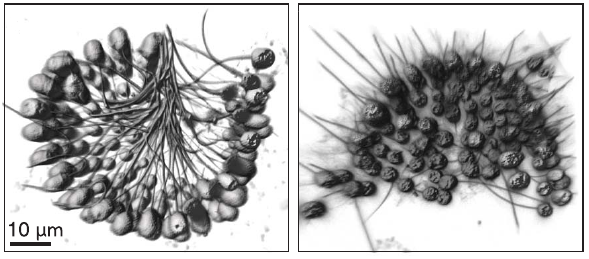
\includegraphics[width=\textwidth]{cflexa.png}
		\caption{}
		\label{subfig:cflexa}
	\end{subfigure}
	\begin{subfigure}[b]{0.43\textwidth}
		\centering
		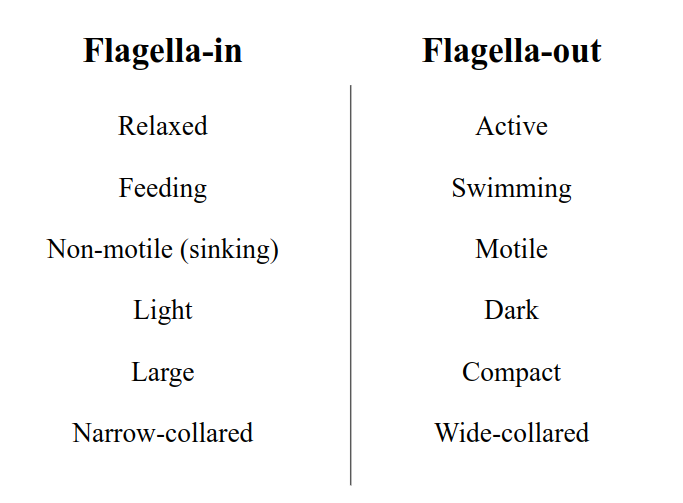
\includegraphics[width=\textwidth]{table.png}
		\caption{}
		\label{subfig:table}
	\end{subfigure}
	\begin{subfigure}[b]{0.57\textwidth}
		\centering
		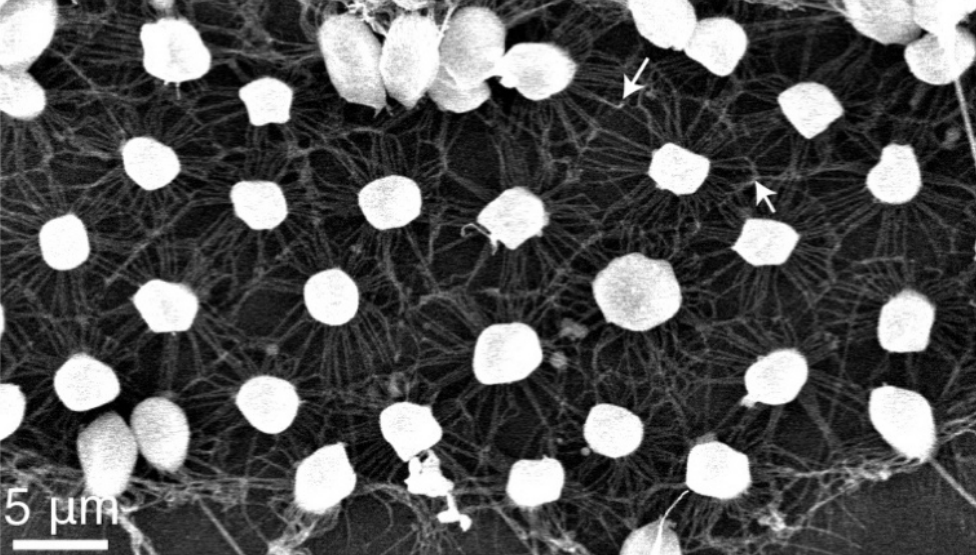
\includegraphics[width=\textwidth]{contact1.png}
		\caption{}
		\label{subfig:contact1}
	\end{subfigure}
	\begin{subfigure}[b]{0.42\textwidth}
		\centering
		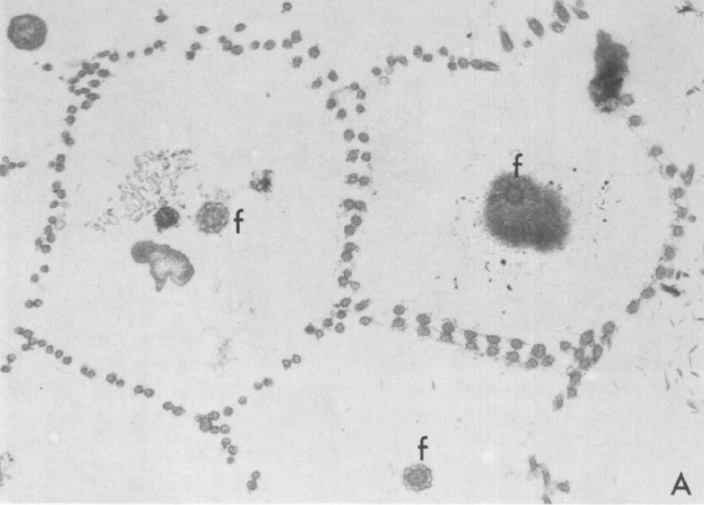
\includegraphics[width=\textwidth]{contact2.png}
		\caption{}
		\label{subfig:contact2}
	\end{subfigure}
	\caption[Overview of \textit{C. flexa} colonies of collared choanoflagellate cells]{Overview of \textit{C. flexa} colonies of collared choanoflagellate cells. (\ref{subfig:cflexa}) Images of the two conformations observed, flagella-in and flagella out. (\ref{subfig:table}) Summary of the two states of \textit{C. flexa} colonies. The transition from flagella-in to flagella-out is induced naturally by darkness, and the reverse transition is induced by the reintroduction of light \citep{brunet2019}. (\ref{subfig:contact1}) Scanning electron micrograph in the tangential plane of a \textit{C. flexa} sheet. Arrows indicate collar-collar contacts. (\ref{subfig:contact2}) Transmission electron micrograph of collar interactions between neighboring cells in a \textit{C. perplexa} colony. f: flagella. From \citet{leadbeater1983} with permission. \cref{subfig:cflexa,subfig:contact1} from \citet{brunet2019}. Reprinted with permission from AAAS.}
	\label{fig:cflexa}
\end{figure} 

% general description
\textit{C. flexa} is an aquatic colonial choanoflagellate that forms sheets on the order of $\SI{100}{\micro\meter}$ in diameter (\cref{fig:cflexa}).
Each cell in a colony consists of a cell body ($\sim \SI{4}{\micro\meter}$), microvillar collar ($\sim\SI{10}{\micro\meter}$ length), and apical flagellum at the collar centre.
All observed sheets have had flagella facing in the same direction, giving the sheet two distinct sides.
Cells attach to each other through their collar microvilli, and in contrast to a colonial flagellate like \textit{S. rosetta}, there is no evidence for an extracellular matrix holding cells together in \textit{Choanoeca} \citep{leadbeater1983,brunet2019}.
Collar microvilli are distinct and colony cells demonstrated no intercellular cytoplasmic bridges (contrast with \textit{i.e. Volvox}), with cells detaching from each other upon treatment with calcium \citep{thibaut}.
\mynote{double check that it was calcium!}
By comparison with division in \textit{C. perplexa}, colony cells are expected to undergo cell division with temporary incomplete replication, where the pair of daughter cells is attached by some shared collar microvilli (\cref{fig:division}).
Colonies are believed to occasionally fragment to separate completely and multiply \citep{leadbeater1983}.

% thecate and division
\textit{C. flexa} also exhibits a sedentary, unicellular form that adheres to surfaces via a stalk (\textit{theca}) without a flagellum, as in \textit{C. perplexa}.
Our understanding of cell division in \textit{Choanoeca} emerges from the thecate form, which leaves one thecate daughter cell and another motile, flagellated cell.
Division begins with the generation of a flagellum by the thecate cell and proceed with protoplasm division with incomplete separation at collar microvilli (\cref{fig:division}) \citep{ellis1930,leadbeater1977}.
The remainder of this work concerns the colonial form of \textit{C. flexa} rather than the thecate or unicellular motile forms.
While we do not have observations on cell replication in the colonial phase, \textit{S. rosetta} gives a suggestion that colonial choanoflagellates do not coordinate their cell division \citep{fairclough2010}.

\begin{figure}[htbp]
	\centering
	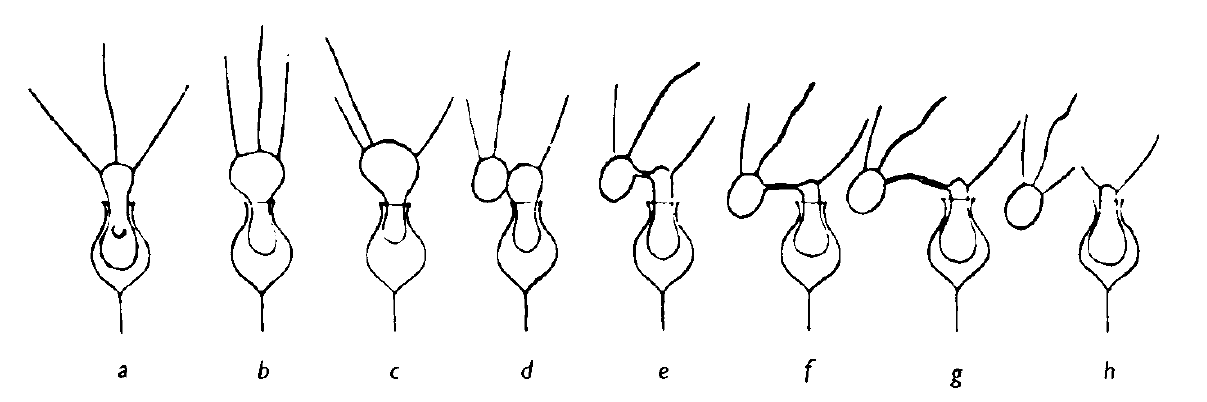
\includegraphics[width=\textwidth]{division.png}
	\caption[Illustrations of stages of division in the sessile form of \textit{C. perplexa}]{Illustrations of stages of division in the sessile form of \textit{C. perplexa}. Reproduced from \citet{leadbeater1977} based on \citet{ellis1930} with permission from Cambridge University Press.}
	\label{fig:division}
\end{figure}

% While choanoflagellate colonies typically orient their flagella to point away from the colony centre, sheets of \textit{Choanoeca} in their rest state point flagella inward. \mynote{cite this! \citet{brunet2019} uses a leadbeater textbook}

\subsection{Sheet inversion}

% inversion introduction
\textit{Choanoeca} has recently sparked renewed interest as a result of the characterisation of rapid light-regulated inversion in colonies, which causes cell sheets to change orientation from pointing flagella-in to flagella-out \citep{brunet2019}.
The inversion is understood to result from contraction of an actomyosin ring at the apical end of colony cells, which results in collar microvilli flaring out. 
This result is consistent with a description of conraction the cell apex with changes in collar angle for \textit{C. perplexa} cells \citep{leadbeater1977}.
Sheet inversion takes $\sim\SI{10}{\second}$.
Notably, deviations in \textit{C. perplexa} collar angle (between $10^\circ-90^\circ$ from the apicobasal axis) were described in \citet{ellis1930}, and \citet{leadbeater1983} described colonies now understood to be \textit{C. perplexa} undergoing inversion. 
\footnote{The latter attributes inversion to a reversal of flagellum rotation, though this explanation is unlikely given the more recent evidence for \textit{C. flexa} \citep{brunet2019}.}
Collar stiffness and the intrinsic curvature in collars facilitates a clear preference in sheet curvature. 
Collars in thecate cells have been described as flaccid \citep{leadbeater1977}, suggesting that an increase in collar stiffness is essential to the transition to colony-forming cells. 

% describing two states
\citet{brunet2019} identified several factors that contribute or prohibit sheet inversion. 
It is believed that, in their natural environment, sheet inversion from flagella-in to flagella-out is triggered by darkness. 
In the inverted (flagella-out) state that occurs in darkness, individual cells demonstrated contraction of an apical actomyosin ring.
The contraction results in collar microvilli flaring out: relative to the apicobasal axis measured at the base of the flagellum, the median collar microvillus angle moved out from $\sim35^\circ$ to $\sim50^\circ$.
This increase in angle is largely the result of collar microvilli straightening out: in light, single colony-cells' collars curve to align with the apicobasal axis after emerging from the apical ends of cells.
\mynote{add figure of individual cells}
Cell sheet area decreases significantly since cell bodies are in contact in the inverted state \citep{thibaut}.
These properties are summarised in \cref{subfig:table}.

% what does inversion achieve?
The transition to the flagella-out state results in a significant increase in swimming speed \citep{brunet2019}. 
In contrast, flagella-in sheets are non-motile to the extent that they typically sink. 
The lack of mobility is compensated by an increase in cells phagocytosed by several times: flagella-in sheets are substantially more effective at driving flow towards the collars, where individual cells feed.
Increased motility in the dark-induced state and accumulation in regions with light facilitates a primitive form of phototaxis.
\mynote{why does swimming not directly translate to feeding as in lauga2011 paper?}

% dynamics
Sheet inversion is rapid and reversible, allowing colonies the flexibility to convert when given suitable environmental cues.
\mynote{discuss how larger sheets are harder to invert}


% Coordinated geometric changes in multicellular organisms are frequent, though they are typically achieved with several differentiated cell types or molecular signalling cascades \citep{todo}. 

% \section{Motivation and objective}
% 
% As in the other basal model organisms used to probe the evolution of multicellularity, \textit{C. flexa} offers a context to study the earliest driving factors towards multicellular shape change through cooperative individual action. 
% In addition to sharing similar geometry with sponge choanocyte chambers and directly informing structural modeling there \citep{asadzadeh2019}, \textit{C. flexa} captures the close relationship between geometry and flow in biological settings. 
% The suspected functionality of its inversion gives a potential evolutionary reason for colony formation in a choanoflagellate.

\section{Thesis overview}

\textit{C. flexa} provides an opportunity to study geometric changes through a simple, uncoordinated mechanism in an evolutionarily basal context. 
In this thesis, I present several approaches for modeling \textit{C. flexa} colony sheets from a mechanics perspective. 
I discuss relevant models from continuous mechanics and find that the simultaneous stretching and compression in several collar microvilli must be taken into account to appropriately model shape and dynamics. 
I review shape equations derived from variation of surface energies defined in terms of curvatures and derive an energy function for a continuous description of \textit{C. flexa} sheets. 

Due to the complexity of the continuous model, I develop a more tractable discrete model based on lessons from the continuous description. 
Collar microvilli are simplified from filaments to elastic rods, which permits a simple energy function to be defined in terms quadratic potentials on cell-collar distances and angles defined by connecting cells and collars.
The model consists of two parameters: equilibrium angles $\phi_0$ (preferred angle from the collar base to the apicobasal axis) and $\psi_0$ (preferred collar-collar contact angle). 
I take the gradient of the energy with respect to cell and collar coordinate vectors as well as the apicobasal axis vectors of all cells to solve the forces acting on all free variables in the system.
I numerically intergrate the forces on all spatial coordinates and torques on cell axes to study dynamics of cell sheets and study their mechanical equilibria.

My discrete model for \textit{C. flexa} colonies successfully models inversion in small sheets consisting of few cells. 
In larger sheets, conformational changes are hindered by rings of cells which cannot undergo the requisite stretching or compression required for inversion or folding. 
% For sheets with too many cells at the boundary, the inability to compress results in buckling at the edges. 
When sheets are already curved with flagella pointing in or out, the inability to sufficiently stretch at the boundary prevents sheets from inverting and causes the cells on the sheet interior to experience substantial stress.
By framing my discrete model of \textit{C. flexa} using graph theory, I identify that the topology of the cell-cell connection lattice determines a sheet's ability to bend without buckling or overstretching.
This finding and my structural results compare well with the understanding of geometric effects of topological defects in crystal lattices.

The model I present makes it possible to identify regions where equilibrium angles $\phi_0$ and $\psi_0$ give minimal energy structures in the flagella-in and -out conformations.
For values that facilitate a flagella-out structure, the flagella-out structure is lower in energy than the flagella-in structure when sheet size prevents inversion as expected.
I argue that the greater amount of time required for larger sheets to invert is the result of a larger energetic barrier or smaller net internal forces, rather than greater hydrodynamic damping through drag. 
This effect from topological constraints at the sheet boundary explains the rapid contraction and slow inversion observed in large sheets in \citep{brunet2019}.
My model supports the hypothesis that \textit{C. flexa} sheets are able to invert as a result of extreme stretching at sheet boundaries or topological changes through collar-collar linkages temporarily breaking.

%!TEX root = ../thesis.tex
%*******************************************************************************
%****************************** Second Chapter *********************************
%*******************************************************************************

\chapter{Continuous model} \label{ch:2}

\ifpdf
    \graphicspath{{Chapter2/Figs/Raster/}{Chapter2/Figs/PDF/}{Chapter2/Figs/}}
\else
    \graphicspath{{Chapter2/Figs/Vector/}{Chapter2/Figs/}}
\fi

Sheets of \textit{C. flexa}, despite being discretely made up of individual cells, appear to take on curvature when looked at as a whole. 
In an effort to develop an analytically tractable model for sheets consisting of many cells and avoid buildilng a detailed network topology, I approximate here sheets of \textit{C. flexa} using continuous functions.

I begin by developing a one-dimensional filament model with inversion dynamics, which demonstrates that azimuthal stretching is key to understanding the flipping process observed in \citet{brunet2019}. 
I proceed to describe a method for approximating sheets of \textit{C. flexa} with two-dimensional surfaces and relate the collar-opening angle $\phi$ and collar-collar contact angle $\psi$ to surface curvature. 
I write an expression for the sheet energy and vary it to derive a shape equation.

\section{One-dimensional model} \label{sec:c_1d}

\mynote{Discuss when a continuous model is appropriate}

We are interested in the problem of \textit{Choaneca flexa} inversion. 
To build intuition, consider a chain of cells connected by their collar filaments like beads on a string. 
Supposing there are sufficiently many cells that the length contributed to the chain of cells by a single cell is small relative to the total length, we approximate the filament with a continuous function $\vec{r}(s)$ parameterised by arclength $s$.
If the filament has preferred curvature $\kappa_0$, then the bending energy functional $\varepsilon$ is given by 

\begin{align*}
    \varepsilon[\vec{r}(s)] &= \frac{1}{2} A \int (\kappa - \kappa_0)^2 ds, 
\end{align*}
\noindent where the curvature $\kappa$ is deduced from $\vec{r}(s)$ and $A$ is the bending modulus. 

If the filament is short relative to the characteristic bending length scale, we express the problem in the Mange representation by writing $\vec{r}(s) = (x, h(x))$ for a height function $h(x)$. 
The resulting energy is written in terms of the prescribed (signed) curvature $H_0$, 
\begin{align}
    \varepsilon[\vec{h}(x)] &= \frac{1}{2} A \int_0^L (h_{xx} - H_0)^2 dx. \label{eq:energy}
\end{align}

Since the cells in this beads-on-a-chain description consist of large spheres connected by thin filaments, we postulate that the filament experiences isotropic drag with coefficient $\zeta$ in a viscous medium.
As a result, we describe the dynamics with a functional derivative of the energy with respect to the changing height,

\begin{align}
    \zeta \vec{r}_t &= -\frac{\delta \varepsilon}{\delta \vec{r}} \nonumber \\
    \zeta h_t &= -\frac{\delta \varepsilon}{\delta h}. \label{eq:eom} 
\end{align}
Taking the functional derivative of equation \ref{eq:energy}, we find the energy change
\begin{align}
    \delta \varepsilon &= \left. A(h_{xx} - H_0)\delta h_x \right|_0^L - \left. Ah_{3x} \delta h \right|_0^L + A \int h_{4x} \delta h ds \label{eq:func_deriv} 
\end{align}
in terms of the boundary conditions of $h$.

For free boundary conditions (force- and torque-free edges) $h_{xx}(0, L) = 0 = h_{3x}(0, L)$, the boundary terms in equation \ref{eq:func_deriv} vanish and we are left with the equation of motion 
\begin{align}
    \zeta h_t &= -A h_{4x}. \label{eq:eom_mange}
\end{align}

Equation \ref{eq:eom_mange} is nondimensionalised by re-expressing $x$ as $x/L$ and $t$ as $t / (\frac{\zeta L^4}{A})$ (the labels $x, t, h, H_0$ are left unchanged for readability) to derive $h_t = -h_{4x}$ with boundary conditions $h_{xx}(0, 1) = 0 = h_{3x}(0, L)$. 
It is clear that the ground state of equation \ref{eq:energy} is given by a quadratic height function with quadratic term $\frac{1}{2}H_0x^2$. 
Let $h_*(x) = -\frac{1}{2} H_0(x-\frac{1}{2})^2 + \frac{1}{8}H_0$ be one such ground state, and suppose $h(x, 0) = -h_*(x)$. Note that the filament in $h(x, 0)$ is not in the ground state since the curvature is given by $H_0$. 

The dynamics of the displacement $g(x, t) = h(x, t) - h_*(x)$ is given by $g_t = g_{4x}$. 
If $g(x, t) = e^{-\sigma t} f(x)$ for some $f(x)$ and eigenvalue $\sigma$, we obtain the ordinary boundary value problem 

\begin{align}
    \frac{d^4f}{dx^4} &= \sigma f & \begin{cases} f''(0, 1) = 0 \\ f'''(0, 1) = 0. \end{cases} \label{eq:bvp}
\end{align}

It is clear that the general solution of $f$ is $A \sin kx + B \cos kx + D \sinh kx + E \cosh kx$ \citep{landau1986}. 
As in \citet{wiggins1998}, the derivatives $f''(0) = f'''(0) = 0$ give $A = D, B = E$. 
Moreover, the eigenvalues $\sigma = k^4$ are given by the sequence of solutions $k_n$ to 

\begin{align}
    \cos k - \frac{1}{\cosh k} &= 0. \label{eq:roots}
\end{align}

Equation \ref{eq:roots} is plotted in Figure \ref{subfig:roots} along with the positions of the solutions $k_n$ as solved numerically. 
The solution $k_0 = 0$ is omitted because it contributes a constant term to $h(x, t)$ that does not evolve in time. 
The eigenfunctions $w_n(x)$ with eigenvalues $k_n^4$ are normalized on the interval $[0,1]$ numerically, and the ratio $A/B$ is given by $(\sinh k - \sin(k)) / (\cosh k - \cos k)$. 
The first five eigenfunctions are shown in Figure \ref{subfig:efuncs}. 

\begin{figure}[tbhp]
    \centering
    \begin{subfigure}[b]{0.48\textwidth}
        \centering
        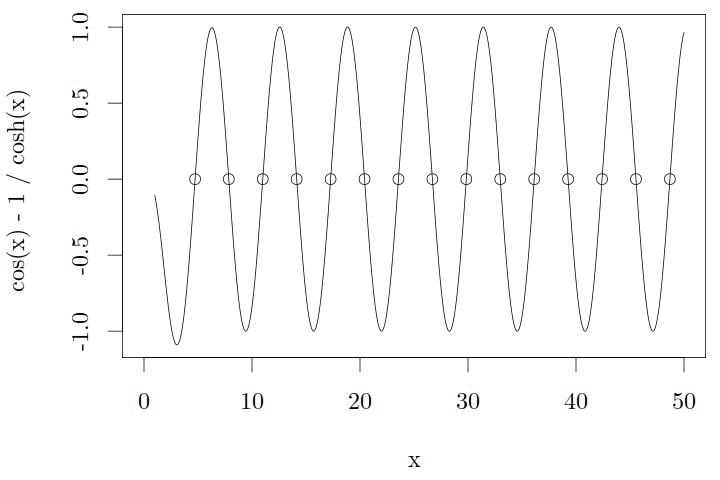
\includegraphics[width=\textwidth]{eq_roots.png}
        \caption{Equation \ref{eq:roots} and its solutions.}
        \label{subfig:roots}
    \end{subfigure}
    ~
    \begin{subfigure}[b]{0.48\textwidth}
        \centering
        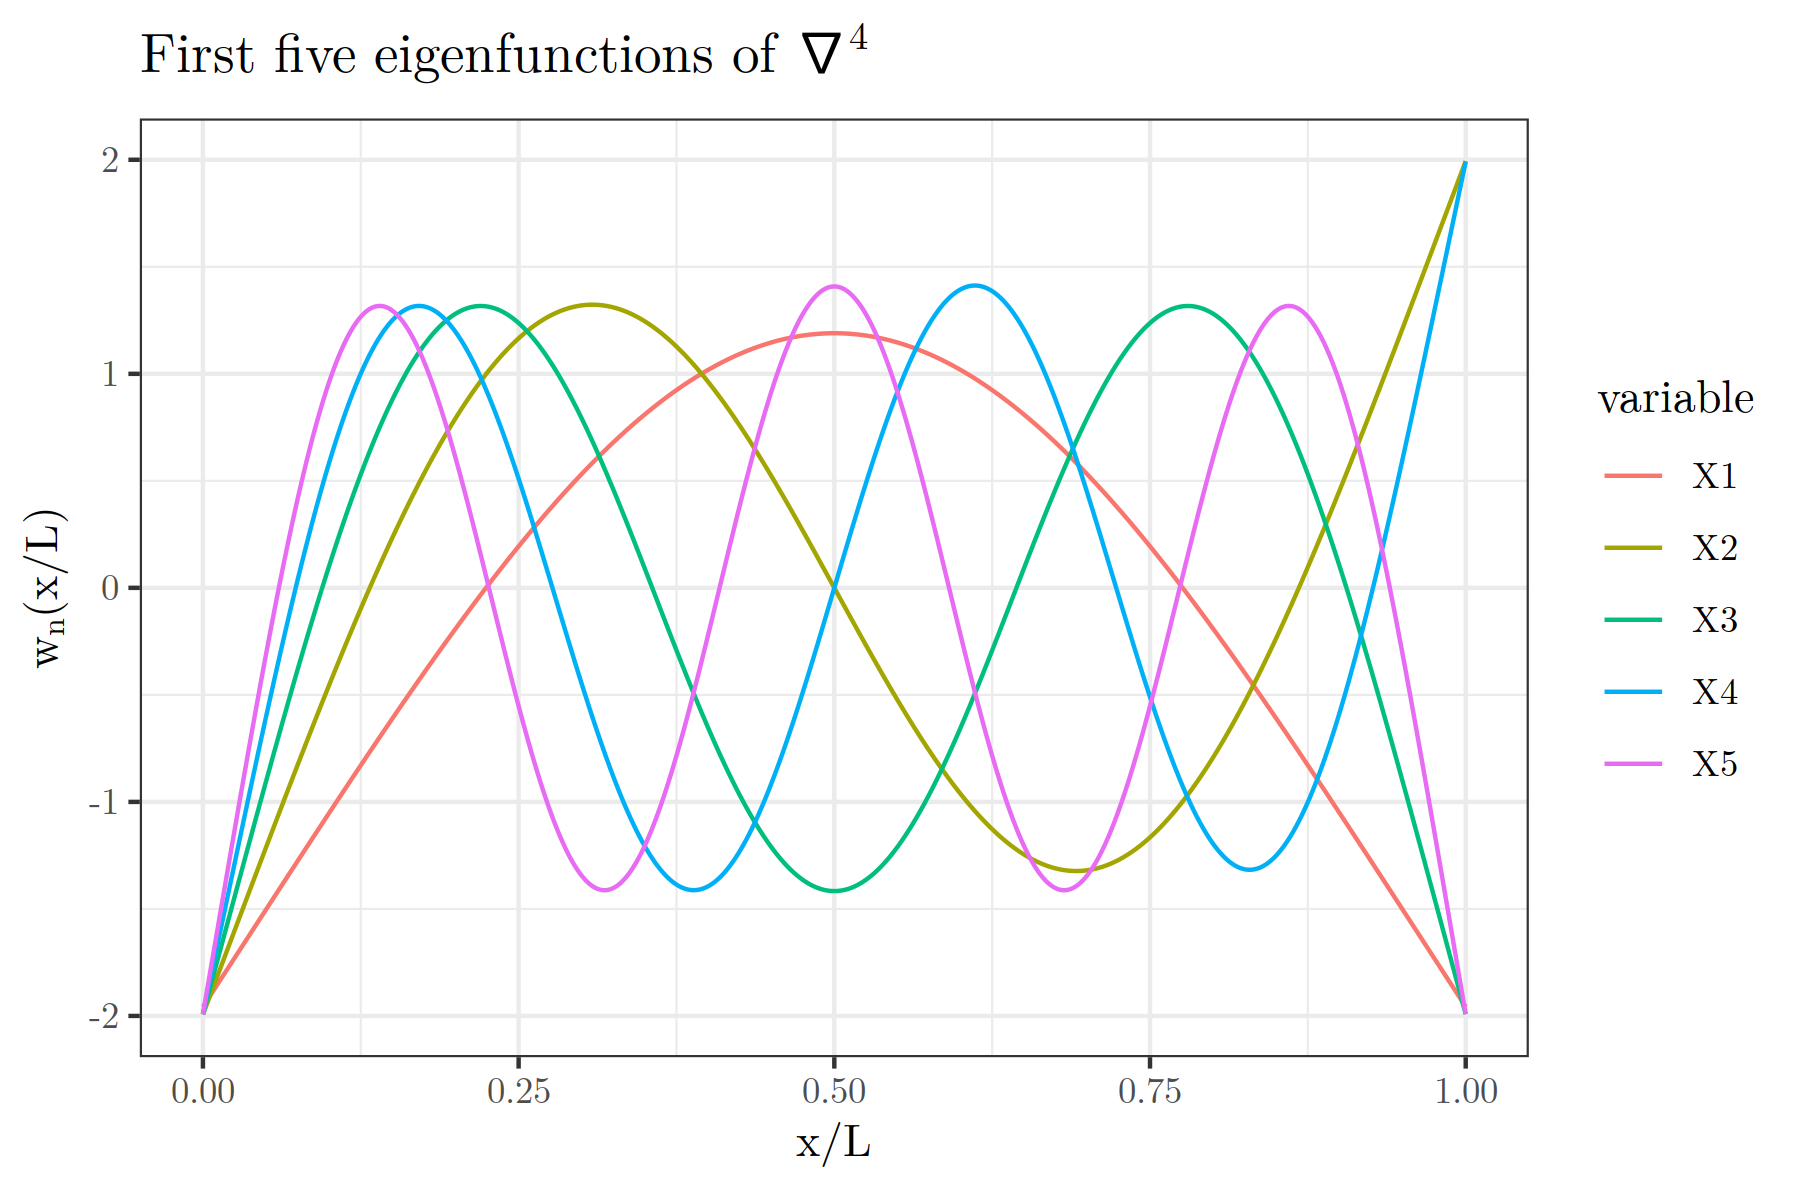
\includegraphics[width=\textwidth]{efuncs.png}
        \caption{The first five eigenfunctions $f_n$ of boundary value problem \ref{eq:bvp}.}
        \label{subfig:efuncs}
    \end{subfigure}
    \caption{Solving the boundary value problem in equation \ref{eq:bvp}}
    \label{fig:bvp_sol}
\end{figure}

Letting $f(x) = \sum_{n=1}^\infty a_n f_n(x)$, we get that $a_n = \int_0^1 g(x, 0) f_n(x)dx$, and the complete dynamics of the height function are given by 
\begin{align}
    h(x, t) &= h_*(x) + g(x) = h_*(x) + \sum_{n=1}^\infty a_n e^{k_n^4 t} f_n(x). \label{eq:sol}
\end{align}
\noindent In practice, only the solutions $k_n$ to equation \ref{eq:roots} shown in Figure \ref{subfig:roots} are used, since the approximation to $h(x, 0)$ is close and higher $k_n$ result in precision errors when calculating $\cosh kx$ and $\sinh kx$. 

For the initial conditions given previously, the time evolution of $h(x, t)$ is shown in Figure \ref{fig:shapes}. 
Immediately, we notice that the filament changes shape extremely quickly, and the timescale $\zeta L^4 / A$ must be extremely large to produce inversion at the order of $\SI{10}{\sec}$ as observed by \citet{brunet2019}. 
Using Stokes' law $\zeta = 6 \pi \mu R$ for dynamic viscosity $\mu$ (about $\SI{1}{\kilo\gram\per\meter\per\sec}$) \citep{stokes1851} and cell radius $R\approx \SI{1e-6}{\meter}$ \citep{brunet2019}, a chain of 100 cells each contributing $\SI{5e-6}{\meter}$ length would require energy constant about 
\mynote{finish the above. compare to bending modulus of flagella or microtubule or somethin} 

Besides the issue of timescale, the dynamics in \cref{fig:shapes} also fail to capture the \textit{rolling over} phenomenon observed at the edges of large sheets \citep{brunet2019}, where a wave of changing curvature propagates from the edge of the sheet towards the centre. 
While the edges show a slight rim around $t\approx\num{9e-4}$, the effect is not as pronounced as in \textit{C. flexa} inversion and does not occur at the initation of the transition.  
A possible explanation for this effect in the cell sheets is that the collars resist compression or stretching. 
The representation used here, on the other hand, does not penalise filament compression.

As the arclength decreases substantially during the transition in \cref{fig:shapes} without affecting its dynamics, it is clear that collar extension and compression are essential to describing appropriate dynamics. Moreover, the timescales between this one-dimensional model and those observed experimentally being as misaligned as they are indicates that some energetic barrier to inversion is missing in the above description. 
We identify here the key deficiency of the one-dimensional description of \textit{C. flexa} sheets, which is that compression and extension, especially in the azimuthal direction, are essential to understand the sheets' bistable nature.

\begin{figure}[bthp]
    \centering
    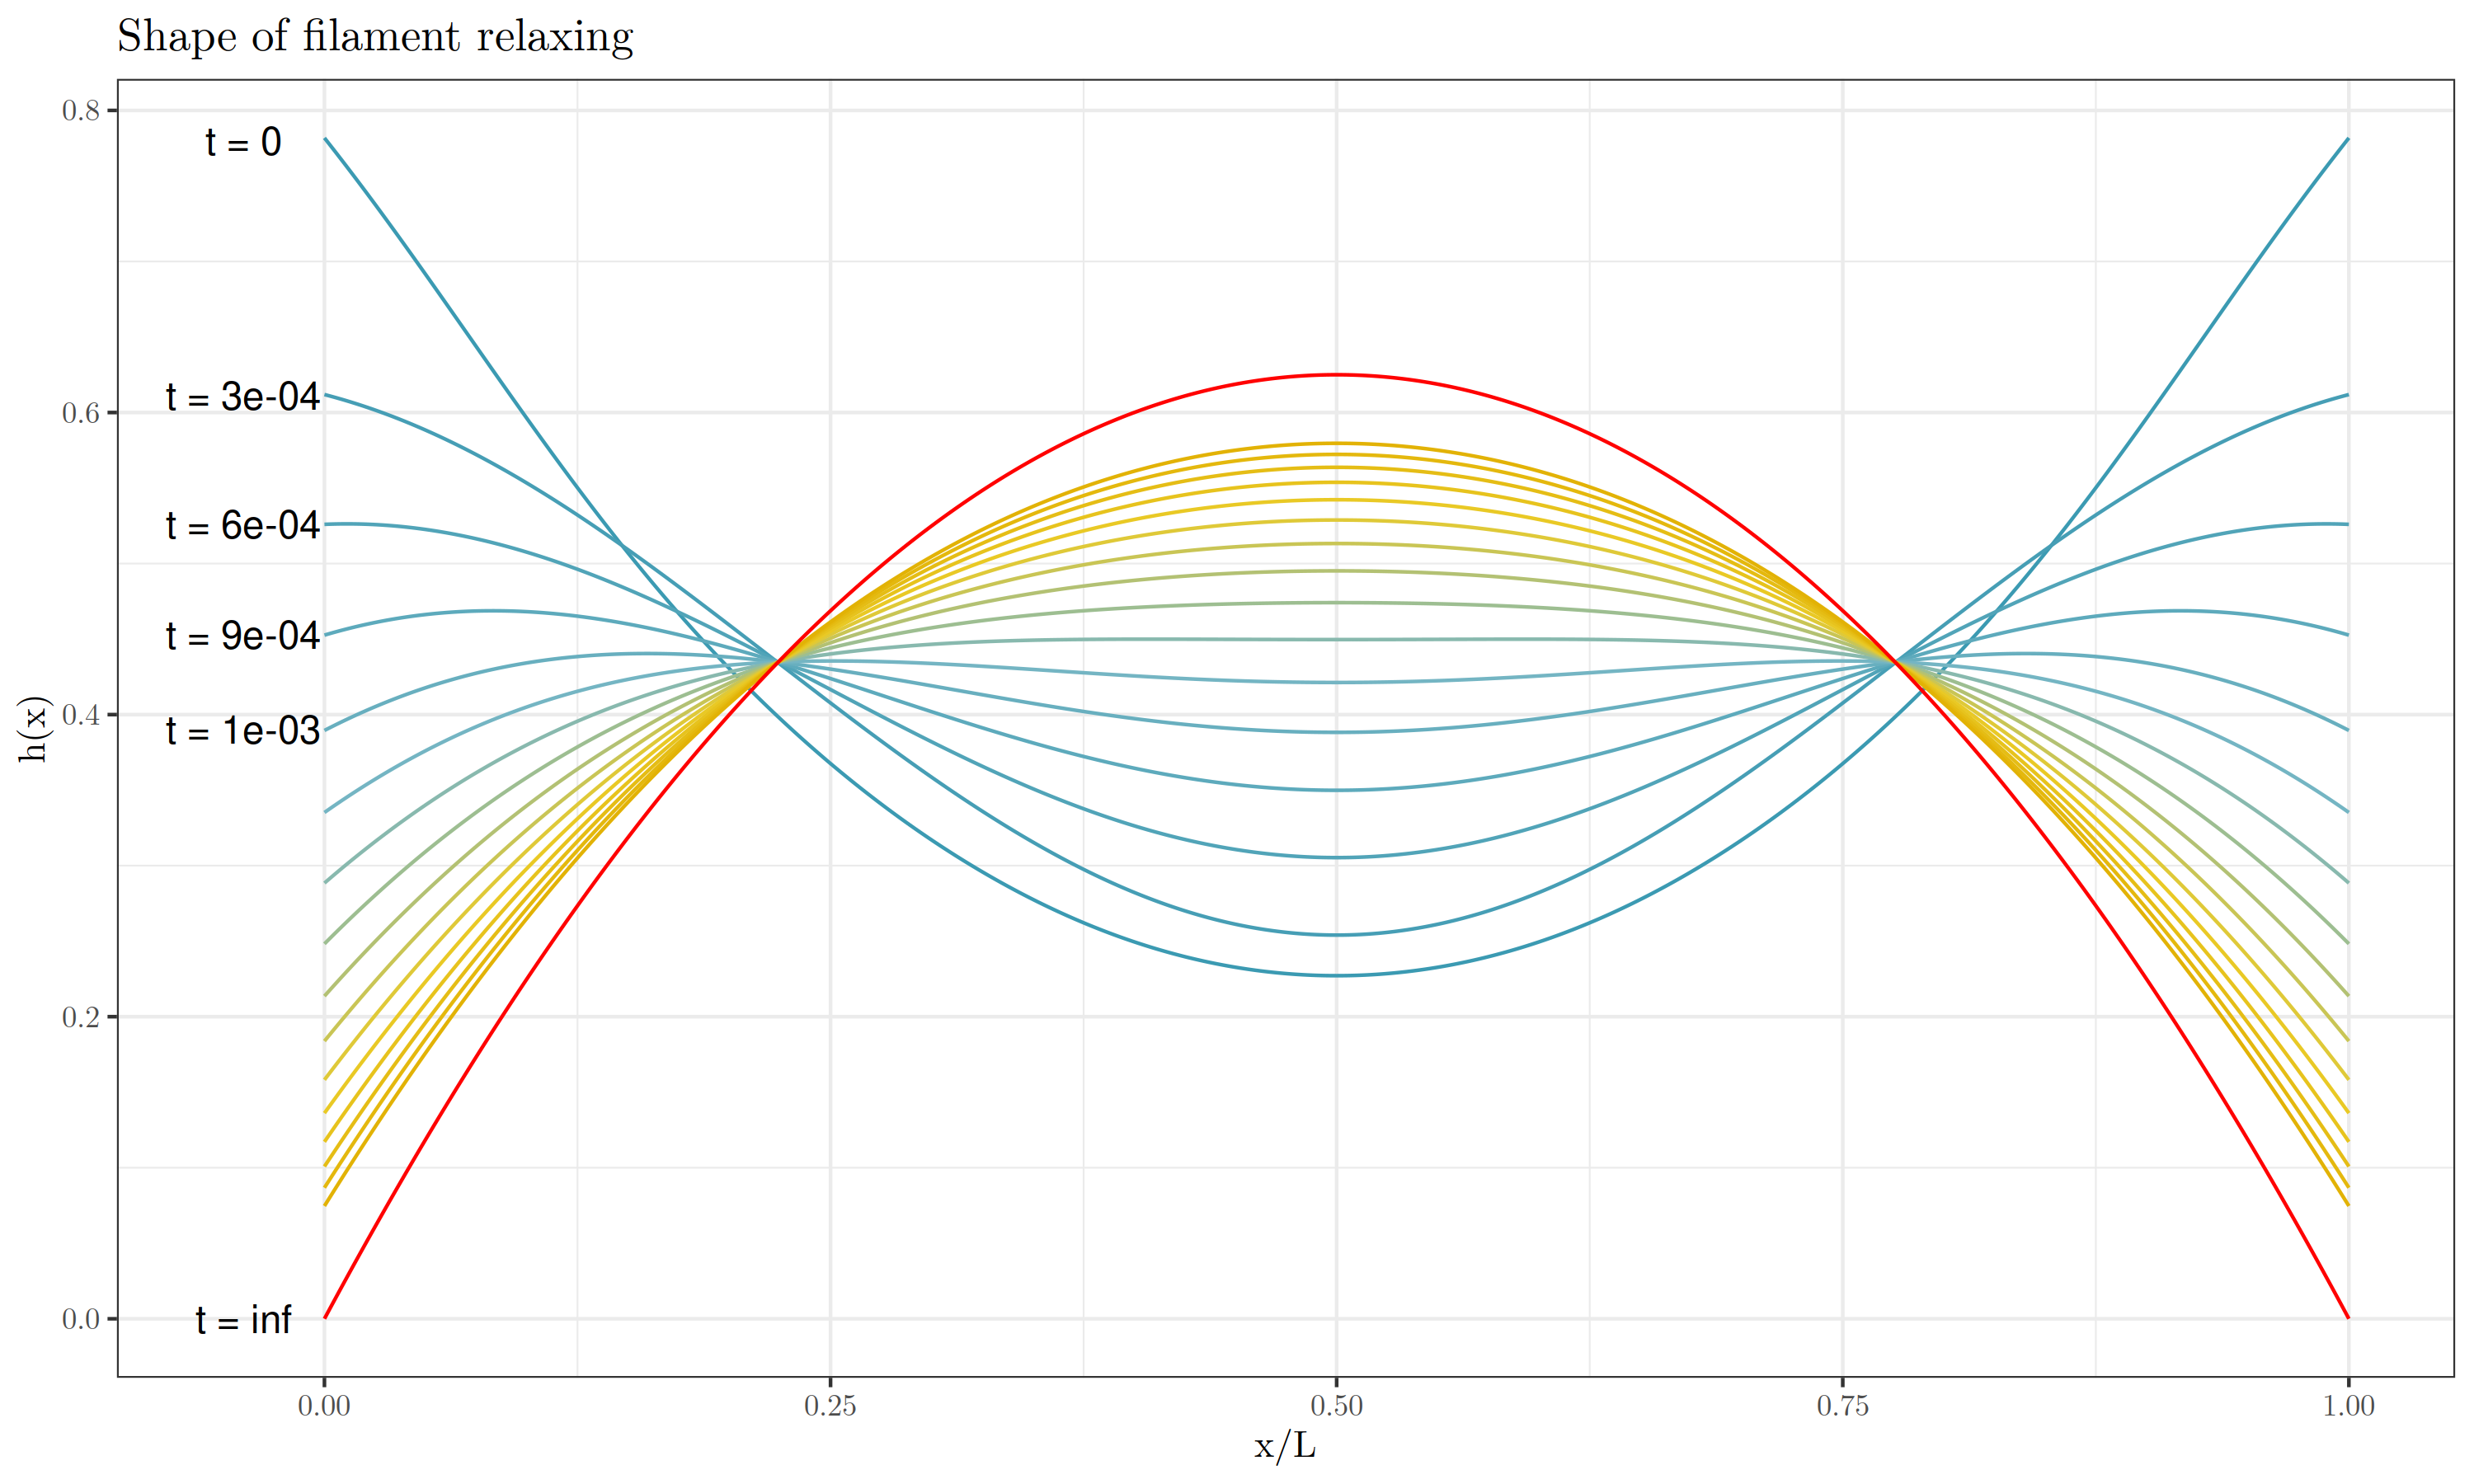
\includegraphics[width=\textwidth]{shapes.png}
    \caption{Time evolution of a one-dimensional filament which switches prescribed curvature sign instantaneously. Time and length are given in dimensionless units defined by the length $L$, bending modulus $A$, and drag coefficient $\zeta$. The time unlabeled time intervals continue sequentially in intervals of $\Delta t = \num{3e-4}$.}
    \label{fig:shapes}
\end{figure}

\section{Surface approximation}

The simplified dynamics that we get from the Mange representation lack energetic costs from the compression and extension that come with deforming a two dimensional surface. The logical step to include these energies is to model the flexa sheet a surface of revolution based on a curve $\bm{r}(\rho, \theta)=(\rho \cos \theta, \rho \sin \theta, z(\rho))$ with cylindrical coordinates $\rho, \theta$ and height function $z$. In doing so, we could take the elastohydrodynamic equation of motion written in terms of curvature $H$ and $K$ and express it as purely as a function of $z$.

We will proceed by writing the equations of motion generally for a surface and reducing it to a surface of revolution.

\subsection{$H$ and collar connection angle}

Before getting into the continuous sheet problem, it is worth describing the two degrees of freedom that our collar connections afford. The collar makes an angle $\phi$ between the vector pointing directly out of the cell and the vector between the cell and its collar boundary with the next cell. Additionally, there is an angle between the collars of two adjacent cells $\psi$. The latter results in the sheet's curvature, so we want to relate it to mean curvature $H$ or preferred curvature $H_0$. 

\mynote{Discuss why we need a collar angle $\psi$ despite \citet{brunet2019} and other sources just talking about $\phi$. This has to do with the straight-collar approximation that I use, where the collar shape and curvature + clamped boundary condition of the meeting collars is distilled into two angles}

\begin{figure}[htbp]
    \centering
    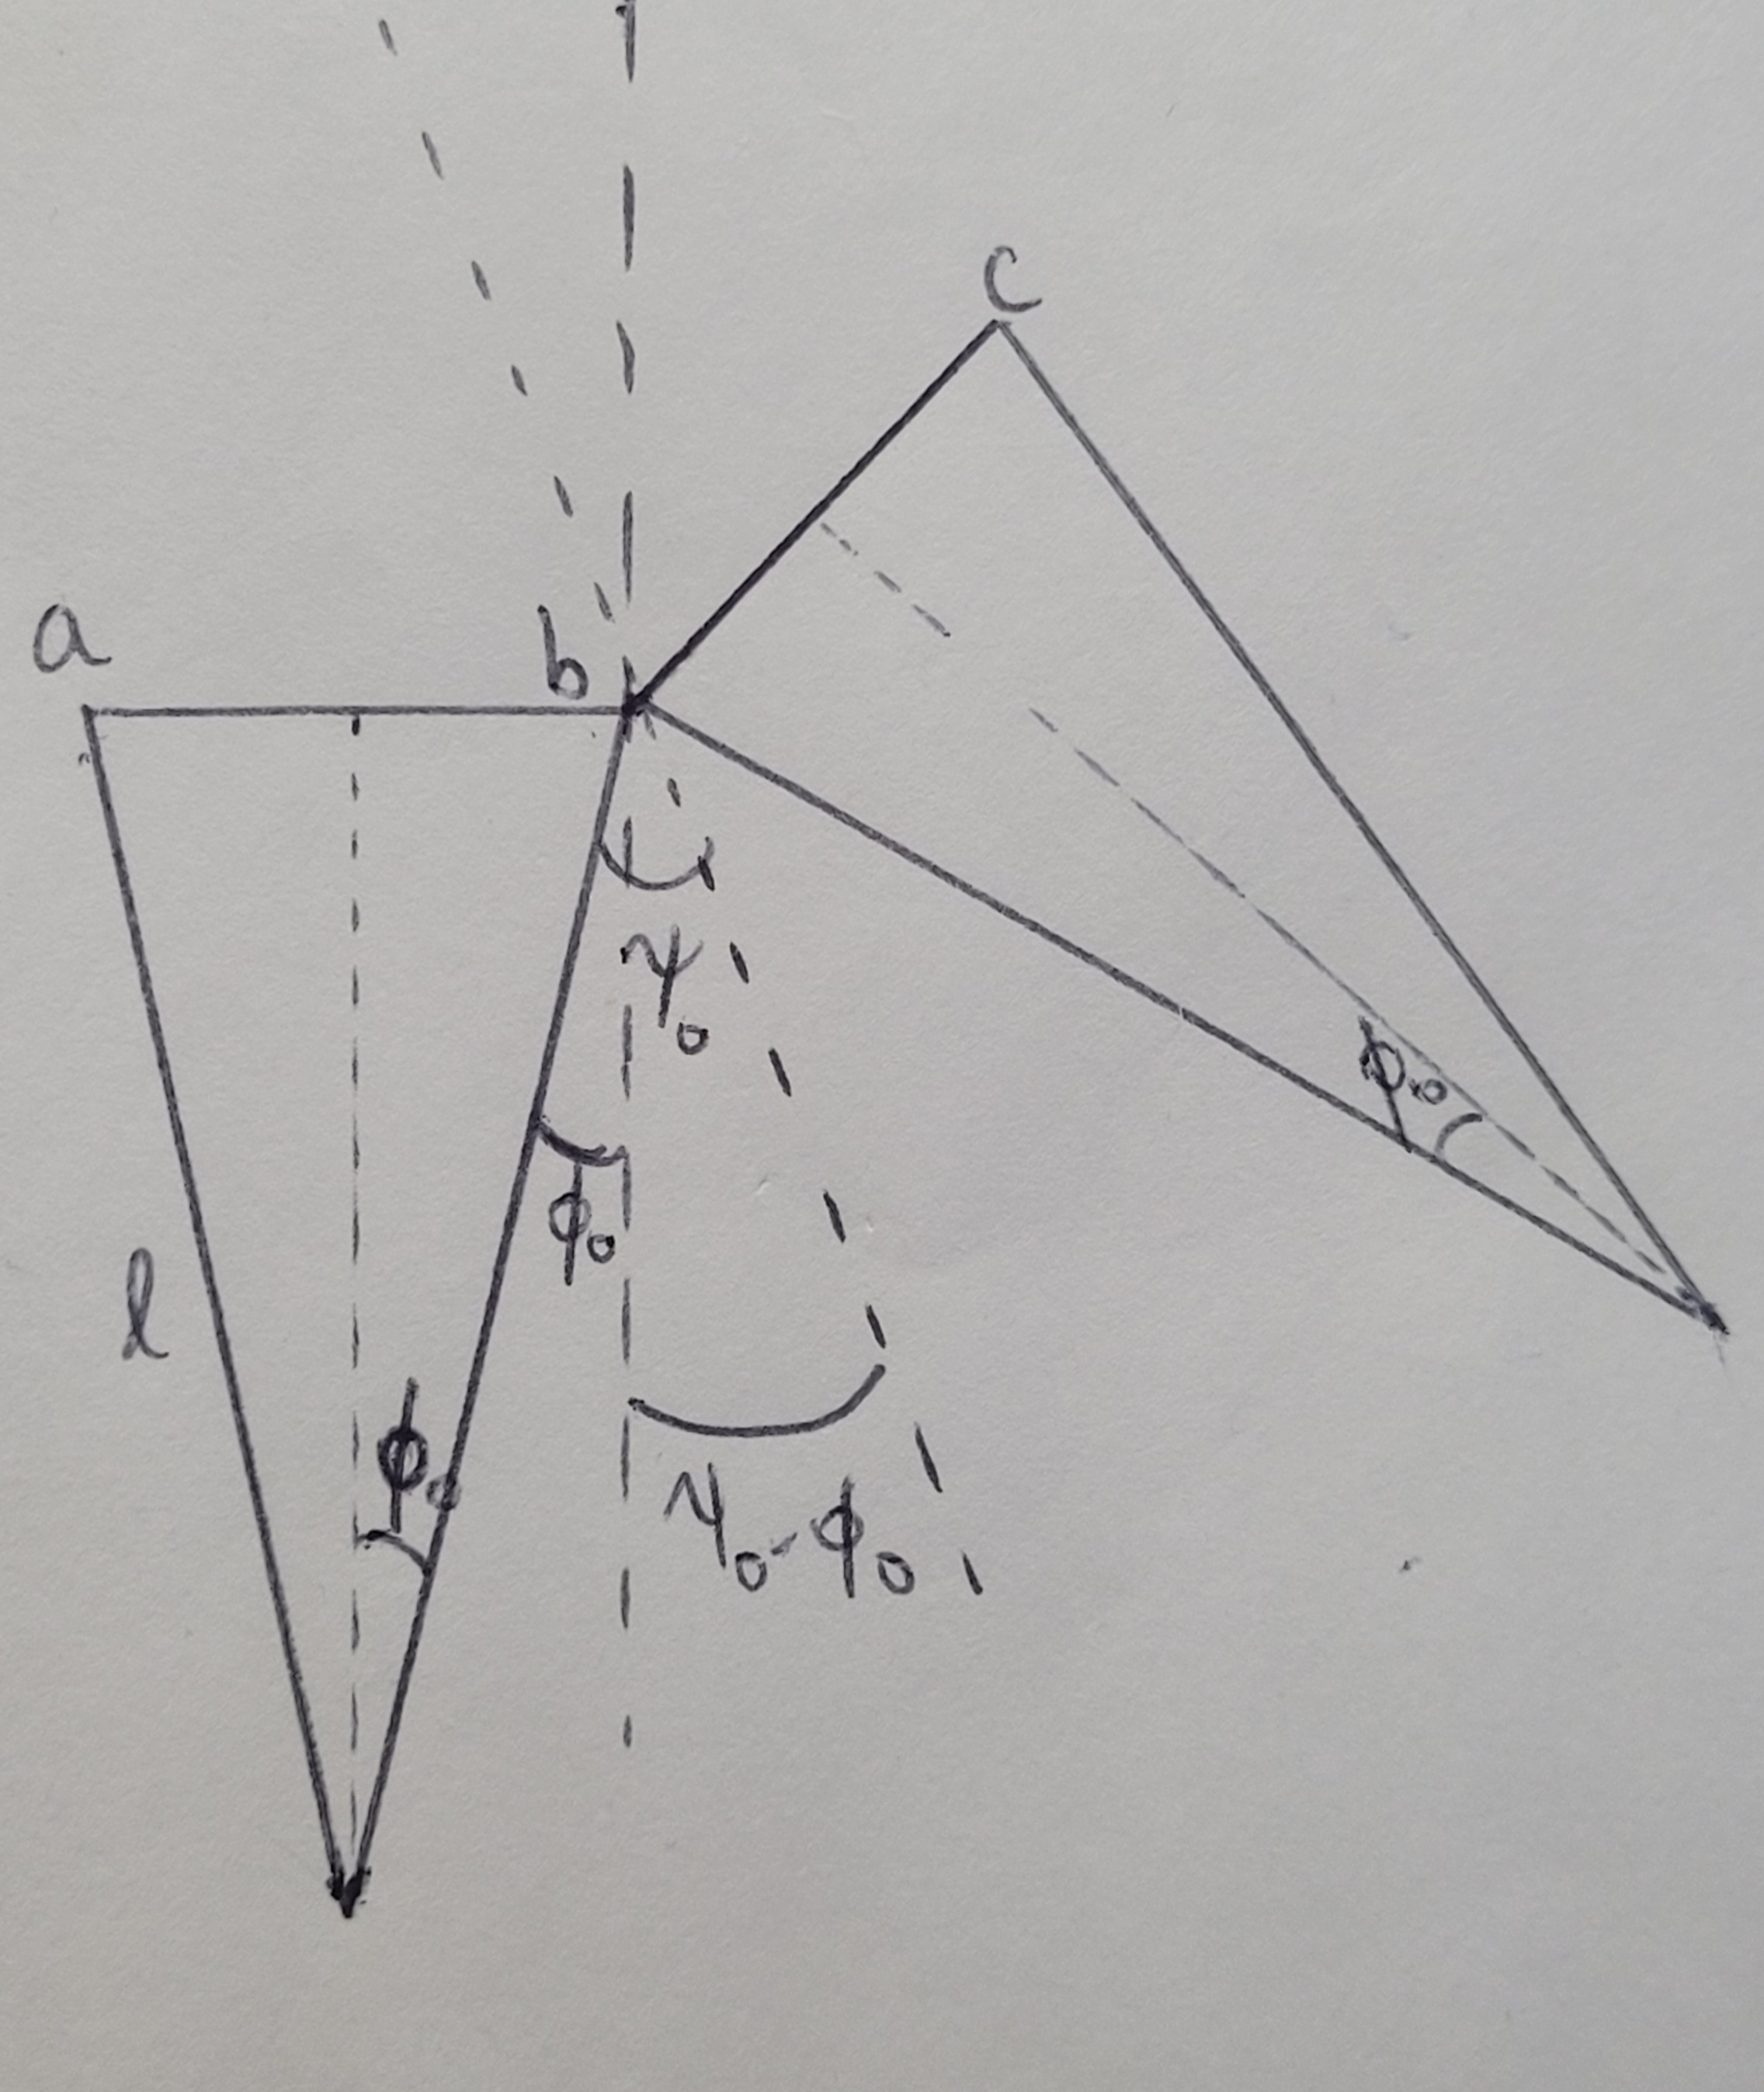
\includegraphics[width=0.5\textwidth]{hpsi.jpg}
    \caption{Geometry for relating collar boundary angle $\psi$ to curvature $H$. }
    \label{fig:hpsi}
\end{figure}

Consider two neighboring cells with collar boundaries $a$, $b$, and $c$, as shown in Figure \ref{fig:hpsi}. We might imagine defining a radius of curvature by the circle that passes through the three collar boundaries. If we set $\bm{x_a} = 2\ell\sin\phi_0(-1, 0)$, $\bm{x_b} = (0,0)$, and $\bm{x_c} = 2\ell\sin\phi_0 (\sin(\psi_0 - \phi_0), \cos(\psi_0-\phi_0)$, we can solve for the circle coordinates 

\begin{align*}
    (x_\circ, y_\circ) &= \ell \sin\phi_0\left(-1, \frac{1+\cos2(\psi_0 - \phi_0)}{\sin2(\psi_0 - \phi_0)} \right)
\end{align*}

\noindent to get the inverse radius of curvature 

\begin{align}
    H_0 = \frac{1}{\sqrt{x_\circ^2 + y_\circ^2}} &= \frac{\sin(\psi_0 - \phi_0)}{\ell \sin\phi_0}. \label{eq:H0_phipsi}
\end{align}

This has a nice, simple interpretation in that if $\psi_0 > \phi_0$, $H_0 > 0$ (as drawn in Figure \ref{fig:hpsi}). On the other hand, $\psi_0 < \phi_0$ implies $H_0 < 0$, or the sheet is concave on the cell body side. 

Alternatively, we solve for $\psi_0$ as a function of $H_0$,

\begin{align}
    \psi_0 &= \phi_0 + \arcsin \left( H_0 \ell \sin \phi_0 \right). \label{eq:h0_psi}
\end{align}

As we find later in equation \ref{eq:hlb}, the curvature of the sheet in any given direction is greater than or equal to $-1/\ell$ (cell bodies and collars cannot go through each other). This lower bound corresponds in \ref{eq:h0_psi} to $\psi_0 = 0$, which we expect when cells are pressing tightly against each other (Figure \ref{fig:maxcurv}).


\subsection{Problem statement} \label{subsec:problem}

\citet{powers2010} (Section IV.B) shows that for an energy density $\e$ written in terms of the first and second fundamental forms $g_{\alpha\beta}$ and $K_{\alpha\beta}$, we can write an expression for the stress tensor $\bm{F}^\alpha$ 

\begin{align}
    \bm{F}^\alpha &= \left(T^{\alpha\beta} + \e^{\alpha\beta}K_\gamma^\beta \right)\bm{t}_\beta - (\nabla_\beta \e^{\alpha\beta})\hat{\bm{n}}. \label{eq:stress}
\end{align}

\noindent Here, $K_\gamma^\beta = K_{\gamma \delta}g^{\delta \beta}$, $\bm{t}_\beta = \partial_\beta \bm{r}$, and 

\begin{align*}
    T^{\alpha\beta} &= g^{\alpha\beta} \e + 2 \frac{\partial \e}{\partial g_{\alpha\beta}} = \frac{2}{\sqrt{g}} \frac{\partial}{\partial g_{\alpha\beta}} \left(\sqrt{g}\e \right) \\
    \e^{\alpha\beta} &= \frac{\partial \e}{\partial K_{\alpha\beta}}
\end{align*}

\noindent with $g = \det{g_{\alpha\beta}}$.

Since the force $\bm{f}$ acting on a surface point is given by the covariant divergence of the stress $\nabla_\alpha \bm{F}^\alpha$, our problem is effectively solved once we decide on an appropriate energy density. \citet{brunet2019} showed that the angle formed by the \textit{C. flexa} collars changes when individual cells are triggered for inversion. We might reasonably suggest preferred sheet curvature is prescribed by changing the preferred angle of the collar $\phi_0$ and imposing and energetic cost based on the amount that the collar angle $\phi(\theta)$ differs around the collar in $\theta$: $\e \sim \int (\phi(\theta) - \phi_0)^2 d\theta$.

\subsection{Connecting continuous surface with individual cell mechanics}

For any point on a smooth surface, we could find an orthonormal basis of eigenvectors $\bm{e}_1, \bm{e}_2$ in the tangent space that diagonalises $K_\mu^\nu$. In terms of a vector $\bm{\Delta \xi}$ written in this basis, we have that the change in height with respect to the tangent plane and its normal $\Delta h$ is given by $K_{\mu\nu}\Delta\xi^\mu\Delta\xi^\nu$.

Let's consider a cell with collar angle $\phi(\theta)$, where $\theta$ measures the location on the collar. If the cell has an optimal collar angle $\phi_0$ and corresponding optimal curvature $K_{0\mu\nu}$, then the height of the collar will be $K_{0\mu\nu}\Delta\xi_0^\mu\Delta\xi_0^\nu$. The distance from the centerline of the cell (the norm of $\bm{\Delta\xi_0}$) is determined by $\phi_0$. The geometry is shown in Figure \ref{fig:geom}.

\begin{figure}[htbp]
    \centering
    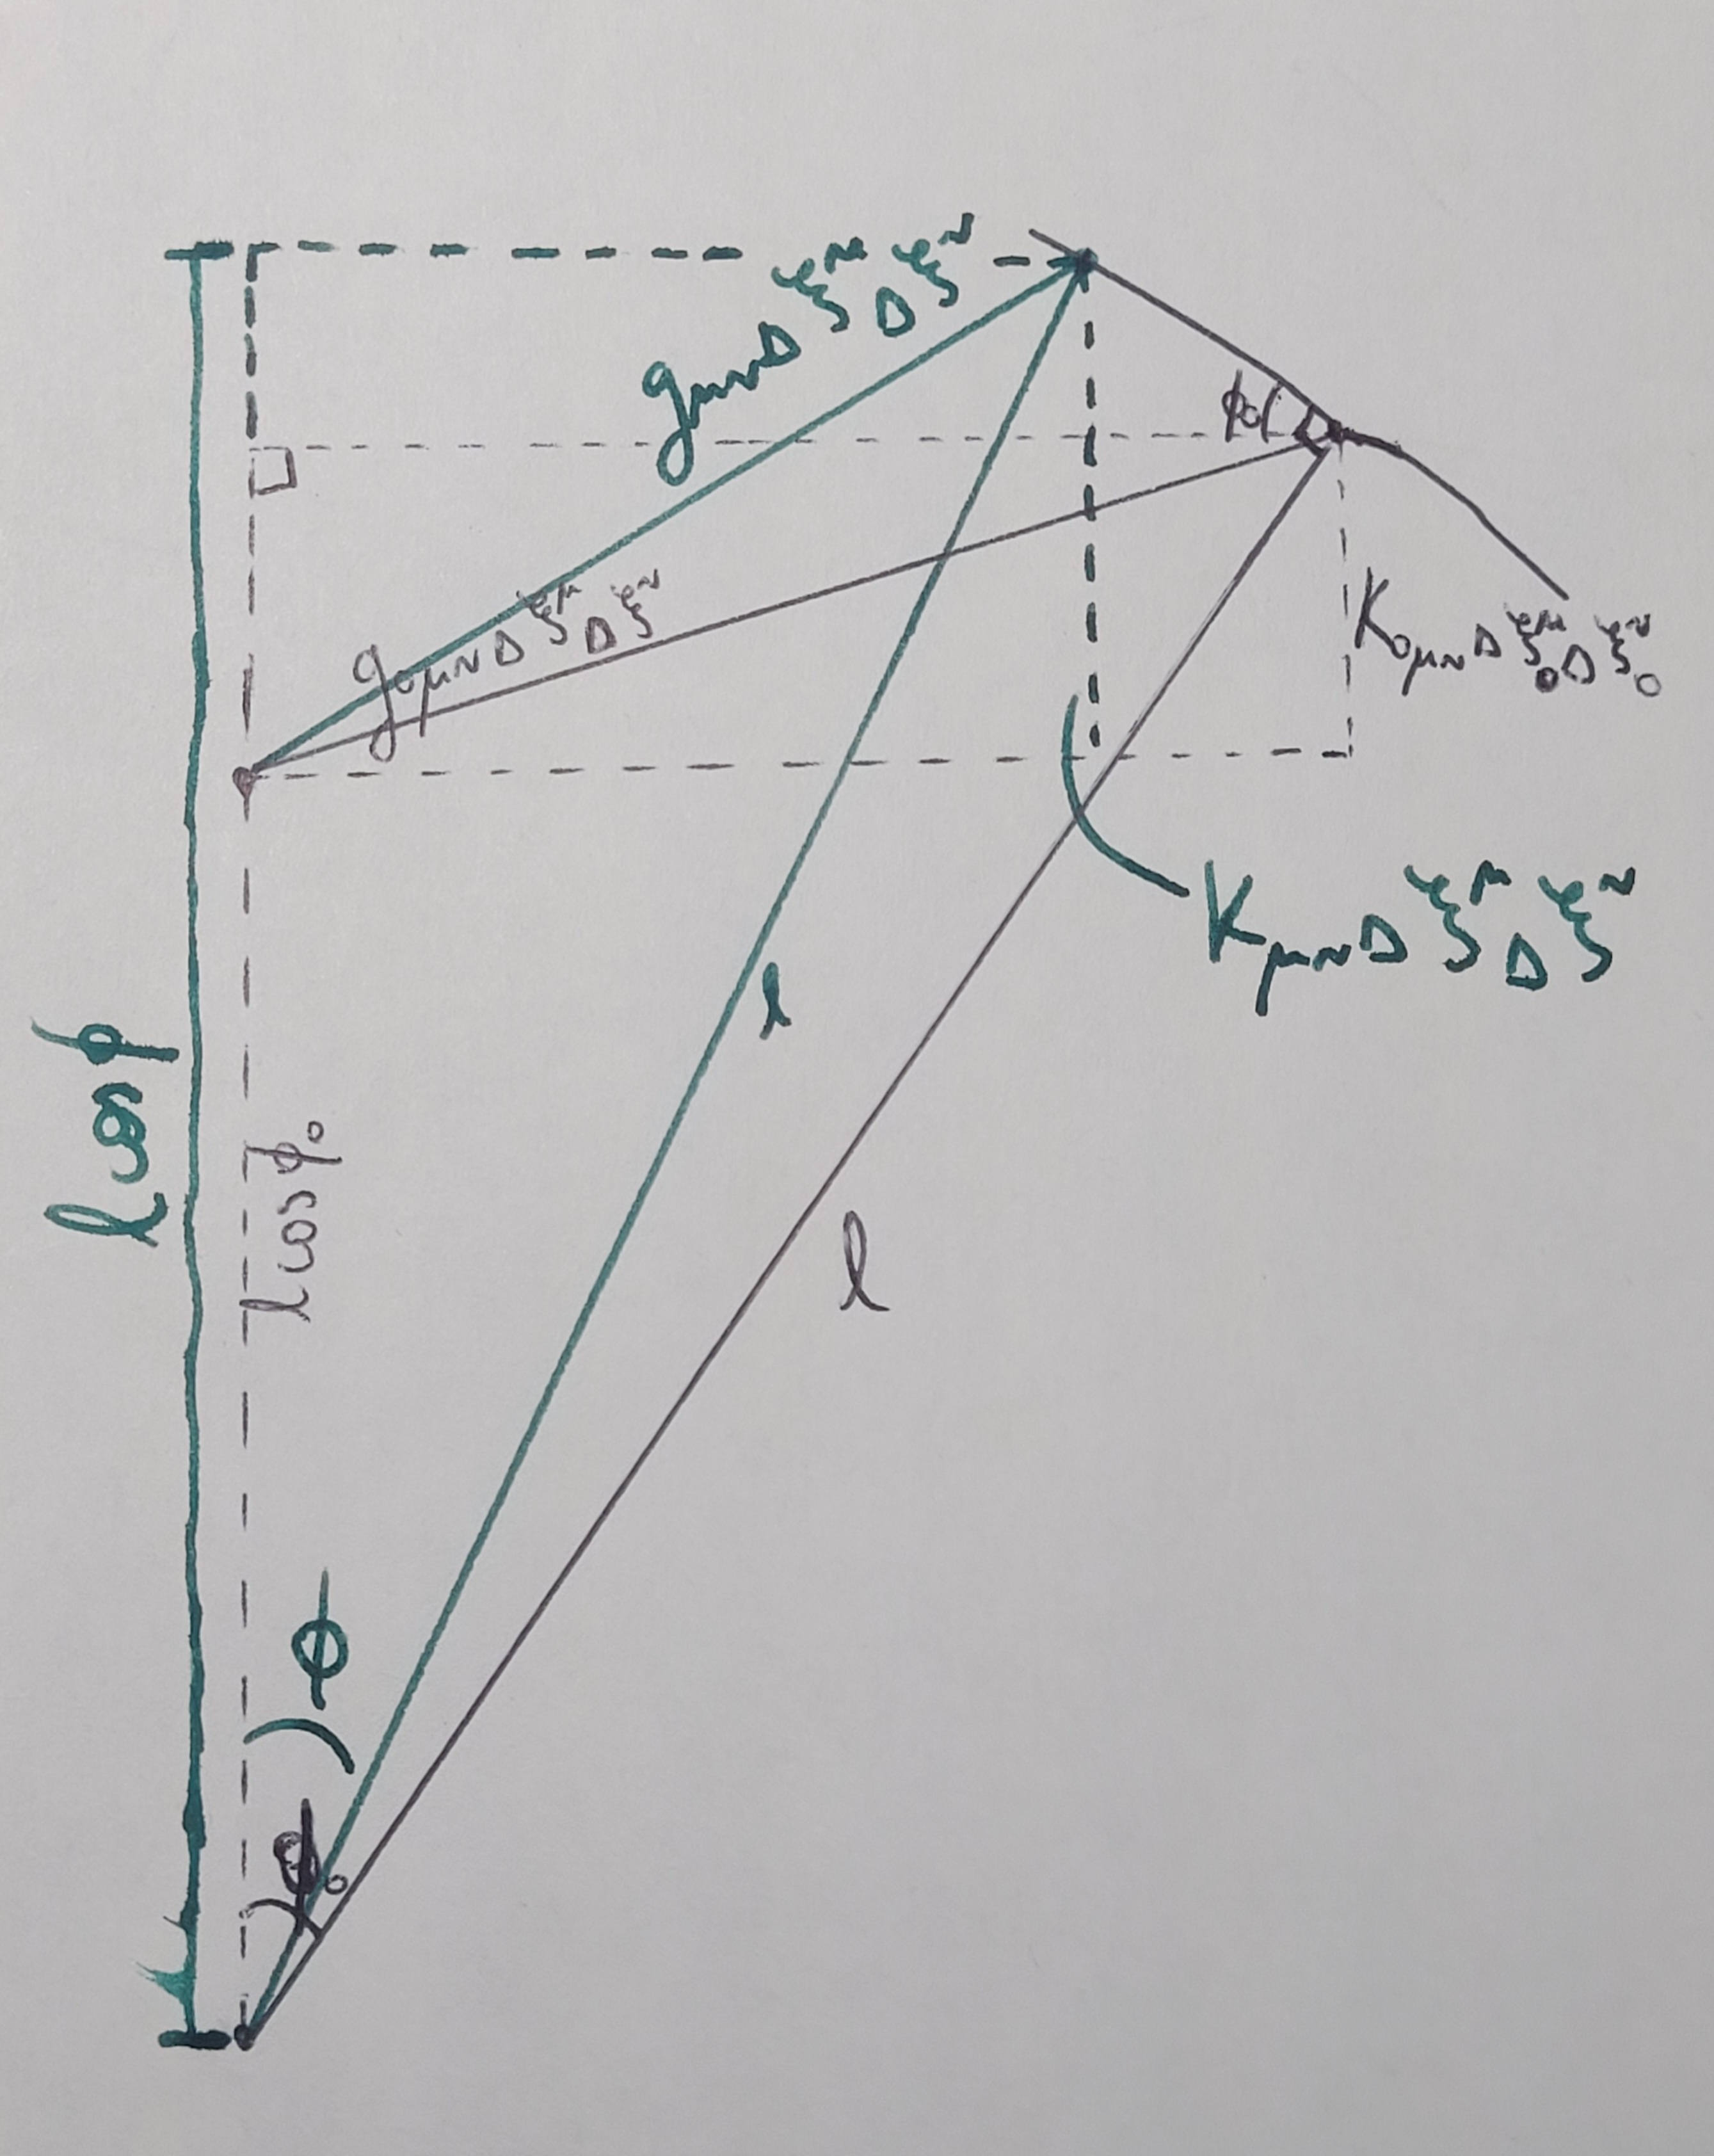
\includegraphics[width=0.75\textwidth]{geom.jpg}
    \caption{Geometry of a single cell and collar with a continuous surface approximating the interactions between collars.}
    \label{fig:geom}
\end{figure}

If the cell has collar angle $\phi$ in direction $\theta$, we know the collar distance as $\bm{\Delta\xi} = \ell(\cos\phi, \sin\phi)$. For a fixed collar length $\ell$, we know the difference in height between the ground state and deformed state is $\ell(\cos\phi - \cos\phi_0)$. We can then relate the collar angle and sheet curvature by equating 

\begin{align}
    K_{\mu\nu}\Delta\xi^\mu\Delta\xi^\nu - K_{0\mu\nu}\Delta\xi_0^\mu\Delta\xi_0^\nu &= \ell(\cos\phi - \cos\phi_0). \label{eq:base}
\end{align}

The radius out from the center for the ground state is $\ell\sin\phi_0$ while for the deformed state it is $\ell\sin\phi$, so for $K_{011}=K_{022}=H_0$, we get

\begin{align*}
    K_{\mu\nu}\ell^2\sin^2\phi (\cos\theta, \sin\theta)^{\mu,\nu} - H_0 \ell^2\sin^2\phi_0 &= \ell(\cos\phi - \cos\phi_0) \\
    H_\theta \ell^2\sin^2\phi - H_0 \ell^2\sin^2\phi_0 &= \ell(\cos\phi - \cos\phi_0)
\end{align*}

\noindent where $H_\theta = K_{11}\cos^2\theta + K_{22}\sin^2\theta + 2K_{12}\sin\theta\cos\theta$ is the curvature of a line on the surface in direction $\theta$. We can cancel a factor of $\ell$, redefine units of length in terms of $\ell$ (such that $H_\theta$ is the ratio of $\ell$ with the radius of curvature in direction $\theta$), and express $\sin^2\phi$ in terms of $\cos\phi$ to get

\begin{align*}
    0 &= H_\theta \cos^2\phi + \cos\phi + (H_0\sin^2\phi_0 - \cos\phi_0 - H_\theta) \\
    \cos\phi &= \frac{-1 \pm \sqrt{1 + 4H_\theta (H_\theta + \cos\phi_0 - H_0\sin^2\phi_0)}}{2H_\theta}.
\end{align*}

If we take the collars to always have angle $0 \leq \phi \leq \pi/2$, we can constrain $0 \leq \cos\phi \leq 1$ to find the two inequalities 

\begin{align}
    H_\theta \geq H_0 \sin^2\phi_0 - \cos\phi_0 \label{eq:ineq1}\\
    1 \geq \cos\phi_0 - H_0 \sin^2\phi_0. \label{eq:ineq2}
\end{align}

\noindent The second inequality can be simplified to $H_0 \geq -(1+\cos\phi_0)^{-1}$. Combining the two inequalities yields 

\begin{align}
    H_\theta \geq -1. \label{eq:hlb}
\end{align}

\noindent Re-expressed with units, this means that $H_\theta \geq -1/\ell$, or that the radius of curvature can never be smaller than $\ell$ on the cells' side. In other words, the cells can't push through each other! (Figure \ref{fig:maxcurv})

\begin{figure}[hbtp]
    \centering
    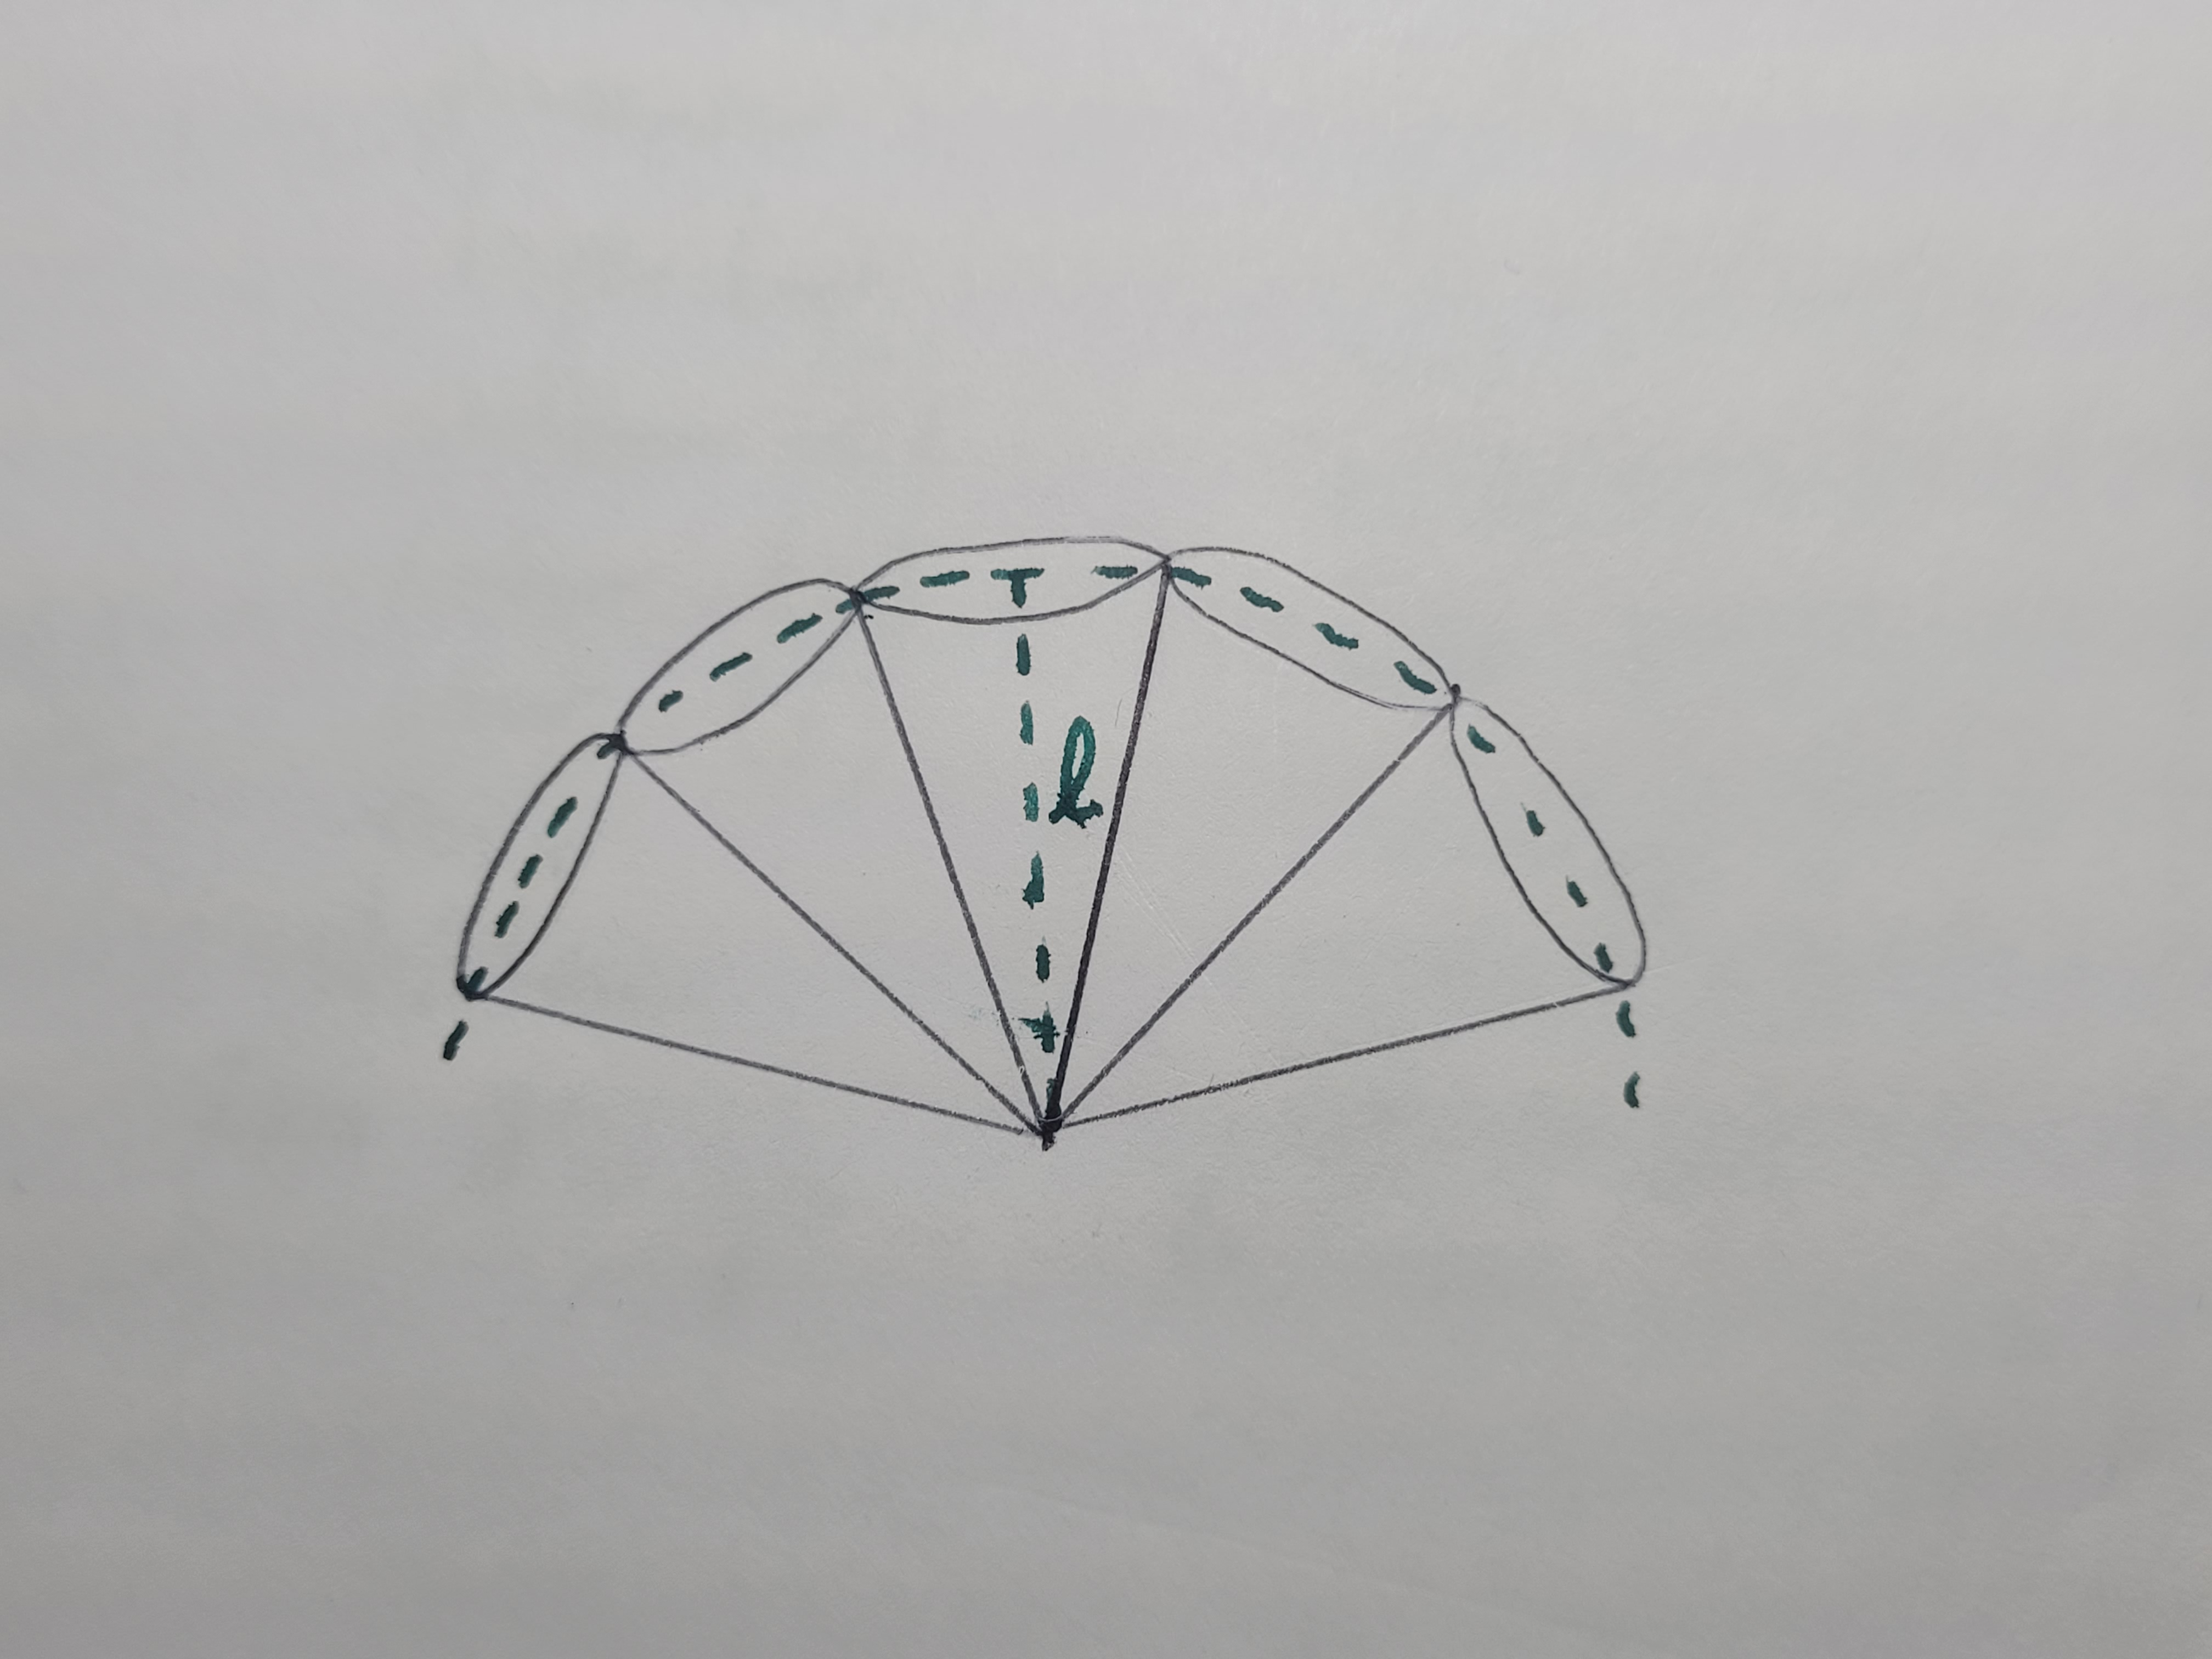
\includegraphics[width=0.5\textwidth]{arc.jpg}
    \caption{Maximum cell-side curvature is given by inequalities \ref{eq:ineq1}, \ref{eq:ineq2} to have radius $\ell$. This corresponds to every (point) cell bumping into each other.}
    \label{fig:maxcurv}
\end{figure}

\subsection{Writing the energy}

We want to write equation \ref{eq:base} in terms of $\phi-\phi_0$ to write down the energy. We can use a trigonometric identity to write

\begin{align}
    H_\theta \sin^2\phi - H_0 \sin^2\phi_0 &= -2 \sin \frac{\phi - \phi_0}{2} \sin\frac{\phi + \phi_0}{2}. \label{eq:preapprox}
\end{align}

\noindent If $phi - phi_0$ is small in magnitude, then 

\begin{align*}
    \sin\frac{\phi - \phi_0}{2} &\approx \frac{\phi - \phi_0}{2} \\
    \sin\frac{\phi + \phi_0}{2} = \sin\left(\phi_0 + \frac{\phi + \phi_0}{2} \right) &\approx \sin\phi_0 + \frac{\phi - \phi_0}{2} \cos\phi_0 \\
    \sin^2\phi = \sin^2\left(\phi_0 + (\phi - \phi_0) \right) &\approx \sin^2\phi_0 +(\phi - \phi_0)\sin2\phi_0.
\end{align*}

Using these approximations we rewrite equation \ref{eq:preapprox} to first order in $\phi - \phi_0$ as

\begin{align*}
    (H_\theta - H_0) \sin^2\phi_0 + H_\theta (\phi - \phi_0)\sin2\phi_0 &= -(\phi - \phi_0) \sin\phi_0 \\
    (H_\theta - H_0) \sin^2\phi_0 &= -(\phi-\phi_0) (H_\theta \sin2\phi_0 + \sin\phi_0) \\
    \frac{(H_\theta-H_0)^2 \sin^4\phi_0}{(H_\theta + \sin\phi_0 / \sin2\phi_0)^2 \sin^2 2\phi_0} &= (\phi - \phi_0)^2.
\end{align*}

We want to integrate this function in $\theta$, so let $K_{11} = a$, $K_{22} = b$, $K_{12} = c$, $-H_0 = d$ and $\sin\phi_0/ \sin 2 \phi_0 = e$ for simplicity when we write

\begin{align*}
    \int_{-\pi}^\pi (\phi - \phi_0)^2 d\theta &= \int_{-\pi}^\pi \frac{\left(a\cos^2\theta + b\sin^2\theta + 2c\sin\theta\cos\theta + d \right)^2}{\left(a\cos^2\theta + b\sin^2\theta + 2c\sin\theta\cos\theta + e \right)^2} d\theta \\
    &= \left\{-\sin2\theta \left[a^2 (-4bc\theta -4ce\theta + d^2 - 2de +e^2) + a(4b^2c\theta -2b(d-e)^2+4c\theta(c^2 - e^2)) \right. \right. \\
    &\qquad \qquad \qquad \left. + b^2(4ce\theta + d^2 -2de + e^2) + 4bc\theta(e^2 - c^2) + 4c^2 (d-e)^2 \right] \\
    &\qquad + 2(a + b +2e) \left[c^2 \theta (b - a) + \theta (a - b) (a + e) (b + e) - c (d - e)^2 \right] \\
    &\qquad \left.+ 2 \theta (a - b)^2 \cos(2 \theta) (a (b + e) + e (b + e) - c^2) \right\} \\
    &\qquad \big/ 2\left[(a - b) (a (b + e) + e (b + e) - c^2) ((a - b) \cos(2 \theta) + a + b + 2 c \sin(2 \theta) + 2 e)\right] \\
    &\quad + \frac{(e - d) (a (4 b + d + 3 e) + b d + 3 b e - 4 c^2 + 2 d e + 2 e^2) \tan^{-1}\left(\frac{-(b + e) \tan\theta - c}{\sqrt{a (b + e) + e (b + e) - c^2}}\right)}{2(a (b + e) + e (b + e) - c^2)^{3/2}}
\end{align*}

\noindent evaluated at $\theta = -\pi, \pi$. Evaluating this expression is surprisingly straightforward, and gives the result 

\begin{align*}
    \int_{-\pi}^\pi (\phi - \phi_0)^2 d\theta &= \text{const.} + \text{const.} \frac{4 K + 2(d+3e)H + 2de + e^2}{(K + 2H + e^2)^{3/2}}.
\end{align*}

Varying this expression will be more difficult than the typical membrane energy defined only in terms of curvature $(H-H_0)^2 + K$ since the Gaussian curvature term is not alone. This means that we cannot use the Gauss Bonnet theorem $\int_S K dA = 2\pi n + \oint_{\partial S}K ds$ to simply write it as a boundary term. Nevertheless, provided that we can vary $K$ on the surface, the shape equation that results shouldn't be very difficult to derive.

\subsection{Varying the energy}

Following subsection \ref{subsec:problem}, we just need to express our energy in terms of $K_{\mu\nu}$ and $g_{\mu\nu}$ to derive a force from it. We of course have that $H = (1/2) (K_{\mu\nu} g^{\mu\nu})$, which is easily differentiated with respect to $K_{\mu\nu}$ and $g_{\mu\nu}$. We can differentiate $K$ by re-expressing it with the identity $K^{\alpha\beta}K_{\alpha\beta} = 4H^2 - 2K$.\footnote{This comes from $4H^2 - 2K = (K^1_1 + K^2_2)^2 - 2(K^1_1K^2_2 - 2K^1_2) = (K^1_1)^2 + 2 K^1_2K^1_2 + (K^2_2)^2 = K^\alpha_\beta K_\alpha^\beta = K^{\alpha\beta}K_{\alpha\beta}$.} Then we have $K = (g^{\alpha\beta}K_{\alpha\beta})^2 - K_{\mu\nu}K_{\alpha\beta}g^{\mu\alpha}g^{\nu\beta}$.

\section{Energy variation}



%!TEX root = ../thesis.tex
%*******************************************************************************
%****************************** Third Chapter **********************************
%*******************************************************************************
\chapter{Discrete model} \label{ch:3}

% **************************** Define Graphics Path **************************
\ifpdf
    \graphicspath{{Chapter3/Figs/Raster/}{Chapter3/Figs/PDF/}{Chapter3/Figs/}}
\else
    \graphicspath{{Chapter3/Figs/Vector/}{Chapter3/Figs/}}
\fi

Models of organisms and population dynamics must be designed by either describing potentially many discrete units\footnote{in this case, cells} with continuous functions or dealing with the analytical complexity of discretisation. 
Even with the continuous description of \textit{C. flexa} described previously, numerical solutions to the shape equations would require discretisation of a surface. 
Here, I pursue a simplified, discrete description of \textit{C. flexa} sheets. 
As in \cref{ch:2}, I proceed by formulating an energy function based on the coordinate vectors of cells and vary it with respect to the coordinates. 
This procedure results in expressions for the forces on the coordinates, which can be forward integrated in time to study the dynamics and steady state geometries of \textit{C. flexa} sheets.

In addition to avoiding the complexity of describing surface curvatures $H, K$ in a discrete program, the discrete approach gives force equations that are relatively quite tractable. 
Expressing the gradient of the energy as summations over collars belonging to each cell or cell-cell interactions makes it possible to neatly arrange the force calculations as tensor index contractions or, even more simply, matrix multiplications. 
The dynamics can efficiently be solved numerically as a result.
Of course, describing choanoflagellate sheets as discrete systems also remains faithful to real sheets, and this approach remains applicable over colonies of arbitrarily many cells.

In \cref{sec:description}, I discuss the reasoning behind the discrete model that I choose to use: why cells and collar boundary endpoints are used as the vertices, how the apicobasal axis unit vector is determined, why collar-collar connections at the sheet boundary matter, and how initial sheet geometries are set up numerically.
The following \cref{sec:sheet_energy} proceeds to write an equation for the mechanical energy of the sheet in terms of cell positions and cell-cell interface endpoint coordinates, as well as the apicobasal axis unit vectors as free variables.
\Cref{subsec:grad_desc}-\ref{subsec:forward_int} proceed to minimise energy by following the negative gradient\footnote{Equivalently, equilibrate forces.}, and the remainder of \cref{sec:minimise_energy} discusses the solutions observed under various sheet graph topologies.


\section{Discrete sheet description} \label{sec:description}

\nomenclature[a-G]{$G$}{Graph consisting of \textit{C. flexa} cells as vertices and cell-cell interactions through collar microvilli as edges}
\nomenclature[a-Gs]{$G^*$}{Graph consisting of collar microvillar interfaces between cells as edges and interface endpoints as vertices}
\nomenclature[g-ps]{$\rho,\sigma$}{Indices used to index collar vertices in the discrete sheet description $\mathfrak{G}$}
\nomenclature[g-ab]{$\alpha,\beta$}{Indices used to index cell vertices in the discrete sheet description $\mathfrak{G}$}
\nomenclature[g-g]{$\gamma$}{Index for either cell ($\alpha,\beta$) or collar ($\rho,\sigma$) vertices in the discrete sheet description $\mathfrak{G}$}
\nomenclature[s-ap]{$(\alpha,\rho)$}{Index for cell $\alpha$ and collar vertex $\rho\subset\alpha$. The set of cell, collar pairs is treated as ordered}
\nomenclature[s-abps]{$(\alpha,\beta:\rho,\sigma)$}{Index for the interface given by collar vertices $\rho,\sigma$ for cells $\alpha,\beta$. The set of these indices is treated as ordered}
\nomenclature[a-n]{$\bh{n}_\alpha$}{Cell body orientation vector for cell $\alpha$. Unit vector}
\nomenclature[a-rvec]{$\bm{r}_\gamma$}{Vector position of vertex $\gamma$}
\nomenclature[x-apvec]{$\vec{\alpha\rho}$}{Vector between vertices $\alpha$ and $\rho$, $\bm{r}_\rho - \bm{r}_\alpha$}
\nomenclature[g-ph]{$\phi$}{Denotes the angle between a cell orientation vector and cell-to-collar vector (\cref{eq:phi}). Indexed $\phi_{(\alpha, \rho)}$ for cell $\alpha$, collar $\rho$}
\nomenclature[g-ps]{$\psi$}{Denotes half the angle between two collar interfaces (\cref{eq:psi}). Indexed $\psi_{(\alpha,\beta:\rho,\sigma)}$ for cells $\alpha,\beta$ and mutual collar endpoints $\rho,\sigma$}
\nomenclature[x-e]{$\e$}{Total sheet energy. In the discrete sheet description, $\e = \e_\phi+ \e_\psi+ \e_{\text{sp}}$ is the sum of energies for angles $\phi$ and $\psi$ and collar length, respectively. An adjustment $\e_\varphi$ is later added for numerical stability.}

The most natural framework to describe a set of interactions between discrete points is graph theory. 
Since colonies of \textit{C. flexa} form sheets with two distinct sides and there is no evidence to suggest that \textit{Choanoeca} acts otherwise \citep{brunet2019,leadbeater1983}, we are welcome to treat the network of interactions between cells as a plane graph $G$. 
With cells $C = \{\alpha\}_{\alpha\in C}$ making up vertices and cell-cell interactions via collars $E = \{(\alpha, \beta)\}_{(\alpha,\beta)\in E}$ making up edges in a graph $G$, we describe which cells impart forces on each other.

However, we understand from the studies into \textit{Choanoeca} that cells interact through their collars \citep{ellis1930,leadbeater1983,brunet2019}. 
Guided by imaging in the sheet-tangential plane (\cref{subfig:contact1,subfig:contact2}), we see that another natural planar graph $G^*$ is that with edges along interfaces between cells' collars.\footnote{Until noted otherwise, I treat the several collars interacting between two cells as a continuous line of interaction with infinitesimal collars spanning the cells' interface. The implications of this choice are discussed later.} 
In this description, vertices mark the points at which the interface between a pair of cells $(\alpha, \beta)\in E$ ends. 
For a cell $\alpha\in C$ whose collar microvilli are all in contact with those of other cells, the vertices in $G^*$ corresponding to cell $\alpha$ are points where $\alpha$ interacts with two or more cells simultaneously.

\begin{figure}[htbp]
    \centering
    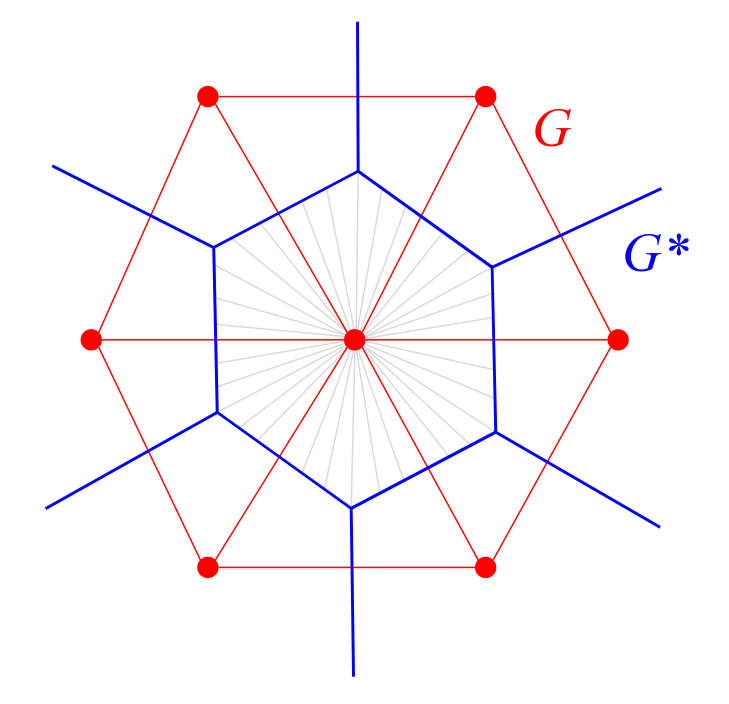
\includegraphics[width=0.6\textwidth]{duals.png}
    \caption[Planar dual graphs describing \textit{C. flexa} colonies]{Planar dual graphs describing \textit{C. flexa} colonies. The graph of cells and cell-cell interactions $G$ shown in red and collar interfaces $G^*$ shown in blue. Compare to \cref{subfig:contact1}, with prominent cell bodies and lines of interface between neighbouring cells' collars.}
    \label{fig:duals}
\end{figure}

As each edge in $G^*$ transects an edge $(\alpha, \beta)$ between cells $\alpha, \beta$ in $G$, we identify $G^*$ as the dual graph of $G$ (\cref{fig:duals}). \footnote{As $G$ is finite, all vertices in $G^*$ as described above which indicate two cells' interactions ending at the edge of a colony sheet would be merged into a single vertex $v_*$ in the dual graph of $G$. Consequently $G^*$ is not exactly the dual graph of $G$. We address this later when defining sheet edges numerically by replacing each edge $(v, v_*)$ in $G^*$ with the edge $(v, v')$ for new vertices $v'$ and removing $v_*$ from $G^*$ and deleting all edges incident on $v_*$.}
Consequently, we have that either $G$ or $G^*$ is sufficient to specify the topology of the other provided the coordinates of vertices. 

For the remainder of this chapter, I will use indices $\alpha,\beta$ to index cell vertices in $G$, indices $\rho, \sigma$ to index collar-collar interface boundary vertices in $G^*$, and index $\gamma$ to index either type of vertex.

\subsection{Defining a sheet} \label{subsec:springs}

A reasonable simplification of the cell sheet will use either the cell-cell interaction graph $G$ or the collar boundary edge graph $G^*$. 
Since physical interactions occur at the collar interfaces, I consider first the physical details of a model defined on $G^*$. 
The following analysis establishes that it is reasonable to consider only the endpoints of lines along which cells' collars interact, at the meeting points of blue lines in \cref{fig:duals}.

If two cells have a collar boundary described by $\bm{r}_\rho t + (1-t)\bm{r}_\sigma$ with $0 \leq t \leq 1$ and the energy is defined by continuously many springs from the boundary to a projected cell point $\bm{r}^*_\alpha$, then the energy $E_{\rho\sigma}$ of that boundary is 
 \begin{align}
     E_{\rho\sigma} = \int_0^1 \left[(\bm{r}_\rho t + (1-t)\bm{r}_\sigma) - \bm{r}^*_\alpha \right]^2 dt &= \frac{1}{3} (\bm{r}_\rho + \bm{r}_\sigma)^2 - \frac{1}{3} \bm{r}_\rho\cdot\bm{r}_\sigma - \bm{r}^*_\alpha \cdot (\bm{r}_\sigma + \bm{r}_\sigma) + \bm{r}^{*2}_\alpha. \label{eq:eab}
 \end{align}

The energy corresponding to a cell consists of the line energies of all the collar interfaces. 
We find the position $\bm{r}^*_\alpha$ by setting the gradient of equation \ref{eq:eab} with respect to $\bm{r}^*_\alpha$ to zero for all lines $\rho\sigma$. 
If $\rho$ indexes the vertices that cell $\alpha$ has (which I denote $\rho\subset\alpha$ for the remainder of this chapter), then 
\begin{align*}
    0 = \frac{dE}{d\bm{r}^*_\alpha} &= -\sum_{\rho\subset\alpha} \bm{r}_\sigma + 2d_\alpha\bm{r}^*_\alpha \\
    \bm{r}^*_\alpha &= \frac{1}{d_\alpha} \sum_{\rho\subset\alpha} \bm{r}_\rho
\end{align*}
\noindent for total stretching energy $E = \sum_{\rho\sigma}E_{\rho\sigma}$ and number of collars $d_\alpha$ belonging to $\alpha$.

The force on vertex $\sigma$ is then given by the negative gradient of the whole sheet energy $E$, which is the sum of the energies corresponding to each cell $\alpha$: 
\begin{align*}
    \frac{d E}{d\bm{r}_\sigma} &= \frac{d}{d\bm{r}_\sigma} = \sum_{\alpha:\sigma \subset \alpha} \frac{d}{d\bm{r}_\sigma} \sum_{\rho \subset \alpha} (\bm{r}_\rho - \bm{r}^*_\alpha)^2. 
\end{align*}
\noindent Since $\bm{r}_\alpha^*$ depends on $\bm{r}_\rho$ itself, we write
\begin{align}
	-\frac{dE}{d\bm{r}_\sigma} &= \sum_{\alpha:\sigma \subset \alpha} \frac{d}{d\bm{r}_\sigma} \sum_{\rho \subset \alpha} \left(\bm{r}_\rho - \frac{1}{d_\alpha} \sum_{\gamma\subset\alpha}\bm{r}_\gamma\right)^2 \nonumber \\
	&= \sum_{\alpha:\sigma\subset\alpha} \sum_{\rho\subset\alpha}\left( 2\bm{r}_\sigma \delta_{\sigma\rho} -\frac{2}{d_\alpha} \sum_{\gamma\subset\alpha}(\bm{r}_\gamma \delta_{\sigma\rho} + \bm{r}_\rho \delta_{\sigma\gamma}) + \frac{1}{d_\alpha^2} \sum_{\upsilon\subset\alpha}\sum_{\nu\subset\alpha} (\bm{r}_\nu \delta_{\sigma\upsilon} + \bm{r}_\upsilon \delta_{\sigma\nu}) \right) \nonumber \\
	&= -2 \sum_{\alpha: \sigma\subset\alpha} (\bm{r}_\sigma - \bm{r}_\alpha^*). \label{eq:com}
\end{align}

\Cref{eq:com} aligns with the expectation that the forces on $\bm{r}_\sigma$ are linear based on the difference to the projected cell points $\bm{r}_\alpha^*$ that $\sigma$ belongs to, owing to the linearity of the entire system.
While the answer may have been readily guessed, the above process of solving for the forces on $\bm{r}_\sigma$ are necessary for nonzero collar length $\ell_0$. 

If instead the line energy is 
\begin{align*}
    E_{\rho\sigma} &= \int_0^1 \left(\left|\bm{r}_\rho t + (1-t)\bm{r}_\sigma - \bm{r}_\alpha^*\right| - \ell_0 \right)^2 dt,
\end{align*}
then the cell position $\bm{r}^*_\alpha$ is the solution to
\begin{align}
	0 &= -2\sum_{\rho\subset\alpha} \bm{r}_\rho + 2d_\alpha \bm{r}_\alpha^* -2\ell_0 \frac{d}{d\bm{r}_\alpha^*} \sum_{(\rho,\sigma) \text{ edge of }\alpha} \int_0^1 \frac{\bm{r}_\alpha^* - \bm{r}_\sigma - t (\bm{r}_\rho - \bm{r}_\sigma)}{| \bm{r}_\rho t - (1-t) \bm{r}_\sigma - \bm{r}_\alpha^*|} dt \label{eq:com_full}
\end{align}

Although the integral in \cref{eq:com_full} can be evaluated analytically, it results in a transcendental equation for $\bm{r}_\alpha^*$. 
Despite the complexity of nonzero equilibrium length for finding a cell position, I nevertheless use the result that continuous spring interfaces can be effectively distilled to interface endpoints (\cref{eq:com}) in the model developed in \cref{subsec:init}.

\subsubsection{Bending} \label{subsubsec:bending}

Points corresponding to cell bodies and collar-collar interface edges make it simple to describe a physically realistic bending energy, though it is not as clear how to define a bending energy.

\citet{seung1988} describe triangulated surfaces and define a bending energy between two triangles $\alpha,\beta$ sharing an interface $\rho, \sigma$ as contributing bending energy $|\bh{n}_\alpha - \bh{n}_\beta|^2/2 = 1 - \bh{n}_\alpha \cdot \bh{n}_\beta$, where all normals face on the same side of the surface. 
Indeed, the continuous approximation of this energy function for small difference $\bh{n}_\alpha - \bh{n}_\beta$ gives the Helfrich energy density $4H^2 - 2K$ \citep{helfrich1973}. 
When cells make boundaries with more than three cells simultaneously, there is not an immediately clear way to define the normal vector $\bh{n}_\alpha$ of a cell $\alpha$. 

As I discuss later (\cref{subsubsec:approx_norm}), a reasonable choice that does not depend on cell position (which in this case is already projected onto the approximated plane of collar positions) would be to approximate $\bh{n}_\alpha$ as the normal vector of a plane approximation to the collar vectices $\bm{r}_\rho$ for $\rho\subset\alpha$. 
Although this choice is intuitively reasonable, it lacks physical motivation as it does not necessarily minimise the energy when the cell body is considered (\cref{subsubsec:opt_norm}).
On the other hand, treating the normal vectors as free variables here would allow them to take any direction to minimise the energy, which does not translate to any physical movement or rotation of the cell body. 

\subsection{Surface formed by cell bodies}

The other natural, minimal discrete description of \textit{C. flexa} is to include only cell coordinates and the network of cell-cell interactions (\cref{sec:description}).
Again, we look to describe the energy contributed by collar stretching and sheet bending.
Unlike the description of bending in \cref{subsubsec:bending}, knowledge of cell body positions gives cell orientation vectors $\bh{n}_\alpha$ a clear physical significance.
Defining the $\bh{n}_\alpha$ as free vectors removes any ambiguity and a bending energy $1 - \bh{n}_\alpha \cdot \bh{n}_\beta$ for two cells $\alpha, \beta$ is reasonable.

On the other hand, considering only cell positions gives no clear method for defining a stretching energy based in a physical mechanism.
We may proceed to define both bending and stretching energy by solving for the minimum energy curves describing two filaments meeting at some mutual point and tangent angle as functions of cell body orientation vectors $\bh{n}_\alpha, \bh{n}_\beta$ and vector $\bm{r}_\alpha - \bm{r}_\beta$ between the two cells.
For any description of cell-cell interactions in \textit{C. flexa} sheet, this approach by treating each collar as a linear filament would likely be the most accurate as it does not require any simplification into angles $\phi, \psi$ (\cref{eq:phi,eq:psi}).
However, this level of complexity removes the interpretational and computational simplicity of distilling the problem as I sought. 
Since neither approach here nor in \cref{subsec:springs} captures all physical interactions in a \textit{C. flexa} sheet with clearly defined terms, I decided to pursue an approach that used details of both collar interactions and cell positions.

\subsection{Numerically specifying initial conditions} \label{subsec:init}

For sheets whose graph of cell-cell connections $G$ can be drawn on a plane with edges as straight lines, it is simplest to define the initial spatial graph $G$ as lying in the $xy$-plane with cell coordinates $\{\bm{r}_\alpha\}_{\alpha\in C}$ and to use Voronoi tessellation to generate collar vertices in $G^*$. 
Voronoi tessellation allows for generalisation beyond regular lattices, though it does not facilitate graph topologies that cannot be drawn in a plane as described above. 

To build more complex graphs $G$ that are nevertheless planar, we can either use subsets of common polyhedra (e.g. subdivided icosahedron) or triangulate points that lie along a surface.\footnote{These topologies are detailed further in \cref{subsec:landscape}.}
In the latter case, I found sufficient flexibility in randomly sampling a specified number of points uniformly distributed on a sphere below some latitude, then calculating the generalised Voronoi tessellation with respect to the metric on the sphere as described in \citet{caroli2010}.
\mynote{add a figure showing the various initial conditions}

We build introduce vertices from $G^*$ where two cells' collar microvilli diverge to build a larger graph $\mathfrak{G}$ consisting of cell-cell interaction edges $(\alpha, \beta)$ from $G$ and cell-collar edges $(\alpha, \rho)$ between cells $\alpha$ and collar edges $\rho \subset \alpha$. 
Here, $\rho \subset \alpha$ denotes a collar vertex $\rho$ from $G^*$ connecting to cell $\alpha$ via the cell's microvilli. 
With cell positions $\bm{r}_\alpha$ already specified and cell-cell interactions given from $G$, collar vertex positions $\bm{r}_\rho$ of collar vertices connecting to three cells are initially set as the centroid of the three cells plus the normal vector of the triangle they form. 
The orientation of the normal vector is set to be consistent across the sheet, such that all collar vertices are positioned on the same side of the sheet, as all cells in \textit{C. flexa} colonies face the same direction.\footnote{Since I use Voronoi triangulation to collar vertices, at most three cells interact at any collar vertex. This is a consequence of the dual of Voronoi tesselation being Delaunay triangulation.}

As Voronoi diagrams for finitely many cells include ridges that extend out to infinity, and the spherical Voronoi algorithm on points below a given latitude on the sphere produces ridge vertices above that latitude, collar vertices at the boundary of the sheet must be added manually. 
I call these collar vertices at the edges as \textit{boundary collars}. Before choosing to add these vertices, we must first consider how collar interactions at the boundary affect sheet energy.

\subsubsection{Boundary collar vertices} \label{subsubsec:bdary_verts}

Do collar-collar interactions at the sheet boundary contribute to the energy?
For boundary cells $\alpha, \beta$, suppose the line of physical interactions between the two cells' microvilli spans from point $\bm{r}_\rho$  and ends at point $\bm{r}_\sigma$. 
We want to know how the angle between the planes given by points $\rho, \alpha, \sigma$ and $\rho, \beta, \sigma$ changes with the position of boundary collar vertex $\sigma$. 

Suppose for the time being that the collar length is fixed at $\ell$, so the possible values for $\bm{r}_\sigma$ are constrained. 
We simplify the problem by reparameterising our coordinates such that $\bm{r}_\alpha = (-1, 0, 0)$, $\bm{r}_\rho = (0, r, 0)$, and $\bm{r}_\beta = (1, 0, 0)$, where $r = \sqrt{\ell^2 - 1}$. 
Here, $\ell$ is a dimensionless ratio of the collar length to half the cell-cell distance. 
We readily see that $\bm{r}_\sigma = (x, y, z)$ is constrained to take values in the circle defined by $r^2 = y^2 + z^2, x=0$. 

Parameterising the positions of $\bm{r}_\sigma(\theta) = (0, r\cos\theta, r\sin\theta)$ by angle $\theta$ with the second axis, we find the normals for planes $\rho, \alpha, \sigma$ and $\rho, \beta, \sigma$ as 
\begin{align*}
	\bh{n}_{\rho\alpha\sigma} &= (\bm{r}_\sigma - \bm{r}_\alpha) \times (\bm{r}_\rho - \bm{r}_\alpha) \\
	&= \frac{(-r^2 \sin\theta, r\sin\theta, r - r\cos\theta)}{r^4\sin^2\theta + 2r^2(1-\cos\theta)}, \\
	\bh{n}_{\rho\beta\sigma} &= (\bm{r}_{\rho} - \bm{r}_\beta) \times (\bm{r}_\sigma - \bm{r}_\beta)\\
	&= \frac{(r^2 \sin\theta, r\sin\theta, r\cos\theta - r)}{r^4\sin^2\theta + 2r^2(1-\cos\theta)}.
\end{align*}
\noindent After simplifying, the angle between these two normal vectors is 
\begin{align}
	\bh{n}_{\rho\alpha\sigma} \cdot \bh{n}_{\rho\beta\sigma} &= 1 - \frac{2}{1 + \frac{1}{2r^2} \left( 1 + \tan^2 \frac{\theta}{2}\right)}. \label{eq:changing_angle}
\end{align}

It is clear that the position of the boundary collar interaction at $\bm{r}_\sigma$ changes the angle between these two planes, given by the arccosine of \cref{eq:changing_angle}. 
In the simplified sheet structure defined in the combined cell-collar graph $\mathfrak{G}$, this results in a change in energy based on the position of $\bm{r}_\sigma$. 
Consequently, as the notation indicates, boundary collar vertices are introduced to $\mathfrak{G}$ connecting between each pair of boundary cells.

\subsubsection{Adding boundary collar vertices}

Defining initial positions for boundary collar vertices becomes challenging when sheets are not planar, though a reasonable placement is sufficient since the positions will be changed later. 
For sheets in the $xy$-plane generated by 2-dimensional Voronoi tesselation (as in \cref{fig:duals}), ridges extending out to infinity are removed and replaced with collar vertices at finite distance. 
The position of a boundary collar vertex $\sigma$ between cells $\alpha, \beta$ for arbitrary starting geometry is calculated as follows. 
First, a unit vector $\bh{n}$ perpendicular to the ridge between cell positions $\bm{r}_\alpha, \bm{r}_\beta$ is determined. 
For sheets in the $xy$-plane, $\bh{n}=\hat{z}$. 
Otherwise, $\bh{n}$ is simply aligned with the average of the normal vectors $\bh{n}_\alpha, \bh{n}_\beta$.
Then, the boundary collar vertex position $\bm{r}_\sigma$ is positioned at the reflection of $\bm{r}_\rho$ over the plane given by points $\bm{r}_\alpha, \bm{r}_\beta, \bm{r}_\alpha + \bh{n}$, where $\rho$ is the existing collar vertex shared by $\alpha$ and $\beta$.
Notably, this process results in a boundary collar position $\bm{r}_\sigma$ farther from the center of the sheet than $\bm{r}_\rho$ and equidistant to $\bm{r}_\alpha, \bm{r}_\beta$ as $\bm{r}_\rho$. 

This process produced reasonable boundary collar vertex positions to initialise sheet dynamics simulations (\cref{fig:layout_init}). 
For initial collar positions not too far from cells, collars would not overlap or cross over each other, even for collars defined with non-coplanar cell positions. 

\mynote{add to figure \ref{fig:layout_init}}

\begin{figure}[hbtp]
    \centering
    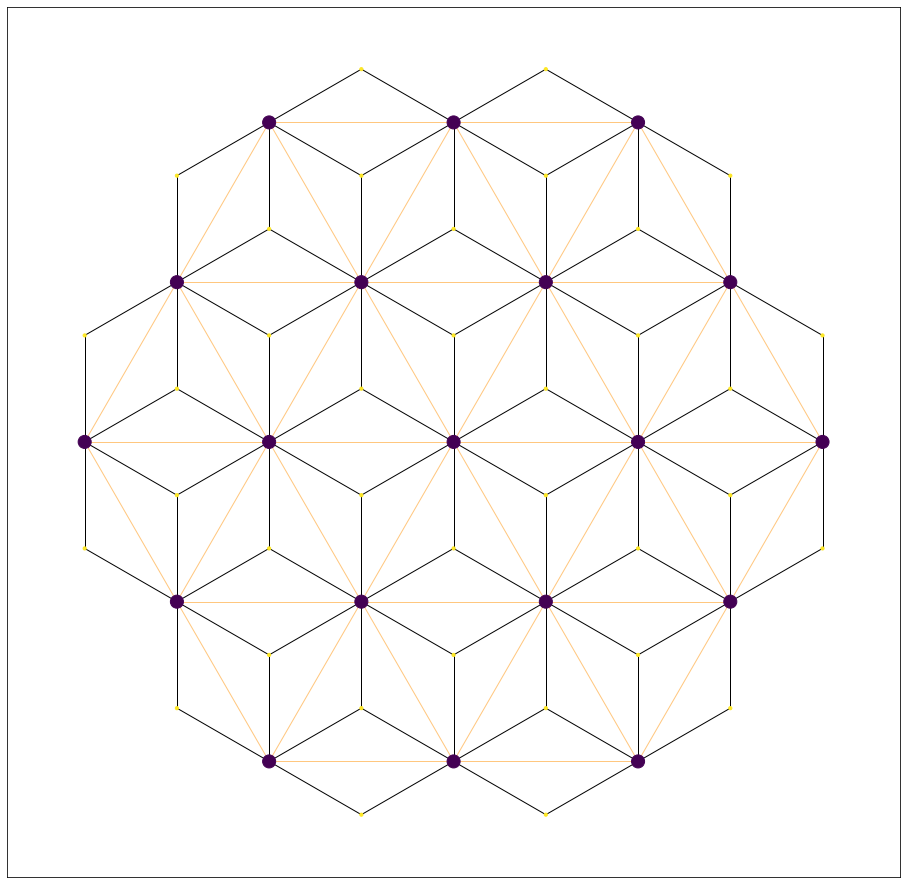
\includegraphics[width=0.8\textwidth]{layout_init.png}
    \caption[Initial layout of the hexagonal lattice flexa sheet]{Initial layout for the flexa sheet projected onto the plane. Cell bodies are shown in large red points and collar boundary vertices are shown in small blue points. Black edges connect cells to collar boundary vertices, and red edges show cell-cell neighbor relations (though these red edges are not physically present). The physical interactions are mediated through the black edges.}
    \label{fig:layout_init}
\end{figure}

\section{Sheet energy} \label{sec:sheet_energy}

\begin{figure}[tbhp]
	\centering
	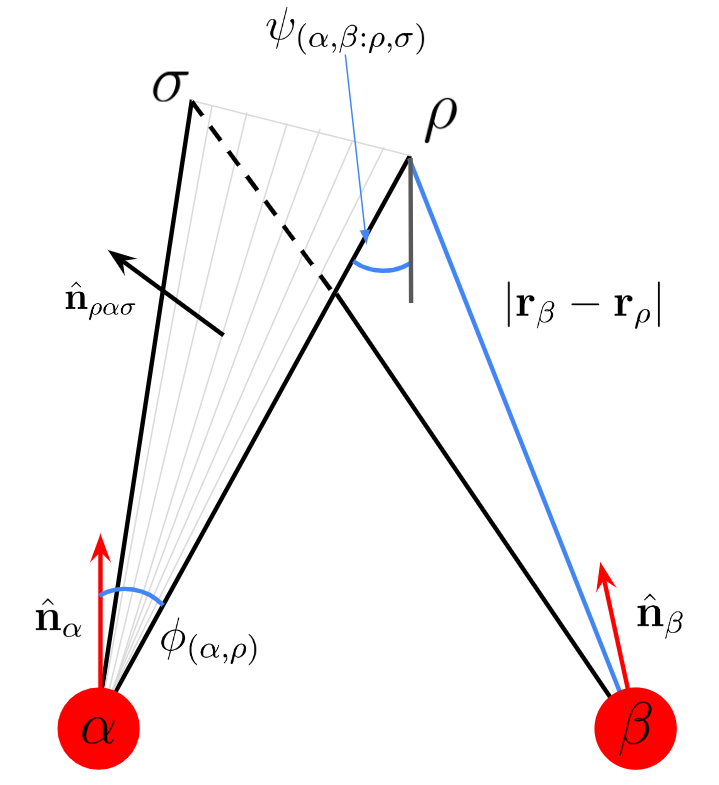
\includegraphics[width=0.6\textwidth]{model.png}
	\caption[Discrete model details]{Detailed view of the discrete model for \textit{C. flexa} sheets shown by the interface between two cells, $\alpha, \beta$ (red), at points $\rho,\sigma$. Cells have unit apicobasal axis vectors $\bh{n}_\alpha, \bh{n}_\beta$, and the plane containing a cell's position $\bm{r}_\alpha$ and two coordinates $\bm{r}_\rho,\bm{r}_\sigma$ belonging to an interface with another cell is defined $\bh{n}_{\rho\alpha\sigma}$. Thin grey microvilli are shown for clarity but not included in the model. The energy (\cref{eq:e}) is defined in terms of angles $\phi_{(\alpha,\rho)}$ and $\psi_{(\alpha,\beta:\rho,\sigma)}$ as well as collar lengths $|\bm{r}_\beta - \bm{r}_\sigma|$.}
	\label{fig:model_details}
\end{figure}

In developing the simplified, discrete model for \textit{C. flexa} as a spatial graph, I aimed to distill the complex physics of collar-collar interactions into a minimum number of sufficient energy terms to capture the sheet bending that we observe experimentally. 
In what follows, I treat edges $(\alpha, \rho)$ between a cell $\alpha$ and collar vertex $\rho$ as straight line collar microvilli and cell pairs, flanking collar pairs $(\alpha, \beta: \rho, \sigma)$ as lines of interactions between the planes given by points $\rho, \alpha, \sigma$ and $\rho, \beta, \sigma$ (\cref{fig:model_details}).
The angles $\phi$ between collar microvilli directions and cell normal vectors and $\psi$ between interfacing collar-cell-collar planes are fully specified by the all cells' coordinates $\{\bm{r}_\alpha\}$, the cells' normal vectors $\{\bm{n}_\alpha\}$ as variables each constrained to have unit length, and the collar interface endpoints $\{\bm{r}_\rho\}$.

Consequently, as detailed in the continuous model description of \cref{ch:2}, I build an energy function $\e = \e(\{\bm{r}_\alpha, \bm{n}_\alpha\}, \{\bm{r}_\rho\})$ that penalises deviations for angles $\phi$ and $\psi$, which describe angles between ($\phi$) collar microvilli and cell normal vectors $\bh{n}_\alpha$, ($\psi$) plane normals $\bh{n}_{\rho\alpha\sigma}, \bh{n}_{\rho\beta\sigma}$, and (sp) collar lengths $|\bm{r}_\alpha - \bm{r}_\rho|$:
\begin{align}
	\e &= \e_\phi + \e_\psi + \e_{\text{sp}}. \label{eq:e}
\end{align}

The terms $\e_\phi$ and $\e_\psi$ capture the energetic penalty incurred by collar bending.
The former results from bending over the length of the collar from the angle formed at the collar base, and the latter captures the bending induced by a neighbouring cell's collars imparting a force.
Moreover, any intrinsic curvature in the collar is captured in the latter term; two filaments each having preferred zero curvature would be in their ground state when the filaments align and cell bodies touch, as in \cref{fig:maxcurv}.
If filaments have intrinsic curvature, the term $\e_\psi$ will encourage distance between cell body positions.
We will see in the following sections that $\e_\phi$ and $\e_\psi$ are functions of all variables $\{\bm{r}_\alpha, \bm{n}_\alpha\}$ and $\{\bm{r}_\rho\}$, while $\e_{\text{sp}}$ is a function only of the spatial coordinates $\{\bm{r}_\alpha\}$ and $\{\bm{r}_\rho\}$.

\subsection{Cell-collar angle energy}
For a physical \textit{C. flexa} cell $\alpha$ with fixed position $\bm{r}_\alpha$ and fixed collar positions $\{\bm{r}_\rho\}_{\rho\subset\alpha}$, we realise that the cell still has freedom in its rotation which we expect will contribute substantially to its energy. 
In other words, there should be an optimal rotation for the cell to minimise its mechanical energy. 
Since we treat \textit{C. flexa} cells as rotationally symmetric above the apicobasal axis, it suffices in our description to assign to each cell $\alpha$ in the graph $\mathfrak{G}$ a unit vector $\bh{n}_\alpha$.
For simplicity, each vector $\bh{n}_\alpha$ is initialised as the unit vector in the direction of $\sum_{\rho\subset\alpha} \vec{\alpha\rho}$, where $\vec{\alpha\rho} = \bm{r}_\rho - \bm{r}_\alpha$.

Defining an energy term on the angle $\phi$ between a cell $\alpha$'s collars and the apicobasal axis $\bh{n}_\alpha$ is done based on descriptions of \textit{Choanoeca} in the literature. 
\citet{brunet2019} describes the change in this angle as the result of exposure to light in \textit{C. flexa}.
Similarly, \citet{ellis1930} characterises the variation in $\phi$ observed in individual cells of \textit{C. perplexa}.

Consequently, we consider an energy term $\e_\phi(\{\bm{r}_\alpha, \bh{n}_\alpha\}, \{\bm{r}_\rho\})$ which penalises devation from a common equilibrium basal collar angle $\phi_0$:
\begin{align}
	\e_\phi(\{\bm{r}_\alpha, \bh{n}_\alpha\}, \{\bm{r}_\rho\}) &= \sum_{(\alpha, \rho)} \left(\phi_{(\alpha, \rho)} - \phi_0 \right)^2. \label{eq:e_phi}
\end{align}
\noindent The sum indicates summation over all cell-collar pairs $(\alpha, \rho)$ in the sheet $\mathfrak{G}$. The angle $\phi_{(\alpha, \rho)}$ is calculated entirely based on the cell normal vector $\bh{n}_\alpha$ and unit vector $\hat{\alpha\rho}$ pointing in the direction of $\bh{r}_\rho - \bh{r}_\alpha$:
\begin{align}
	\phi_{(\alpha, \rho)} &= \arccos \left(\bh{n}_\alpha \cdot \hat{\alpha\rho} \right) = \arccos \left(\bh{n}_\alpha \cdot \frac{\vec{\alpha\rho}}{\left| \vec{\alpha\rho}\right|} \right). \label{eq:phi}
\end{align}

\subsubsection{Optimal cell normal vectors} \label{subsubsec:opt_norm}

No other energy terms will depend on the cell normal vectors $\{ \bh{n}_\alpha \}$, so we ask now what the optimal normal vector for a cell is. Suppose a cell is at position $\bm{r}_\alpha$ with collar vertices at $\bm{r}_\rho$ for $\rho \subset \alpha$. We can determine how the cell orients in order to minimise the collar energy with respect to $\bh{n}_\alpha$. 

For fixed $\alpha$, the cell orientation vector $\bh{n}_\alpha$ is constrained to have unit length. Hence, we solve the constrained optimisation of $\e_\phi$ by solving the Lagrange multiplier problem with multiplier $\lambda$
\begin{align}
    0 &= \frac{\partial \left[ \e_\phi + \lambda\left( \left| \bh{n}_\alpha\right|^2 - 1\right) \right] }{\partial \bh{n}_\alpha} \label{eq:philagrange1} \\
    0 &= \frac{\partial \left[ \e_\phi + \lambda\left( \left| \hat{\bm{n}}_\alpha\right|^2 - 1\right)\right] }{\partial \lambda}. \label{eq:philagrange2}
\end{align}

Using the constraint (solution to \cref{eq:philagrange2}) $| \bh{n}_\alpha |^2 = 1$, we solve 
\begin{align*} 
    \lambda \bh{n}_\alpha &= 2 \sum_{\rho\subset\alpha} \left[ \arccos\left(\hat{\alpha\rho} \cdot \bh{n}_\alpha \right) - \phi_0 \right] \frac{-1}{\sqrt{1 - \left(\hat{\alpha\rho} \cdot \bh{n}_\alpha \right)^2 }} \hat{\alpha\rho} \\
    \lambda &= 2 \left| \sum_{\rho\subset\alpha} \left[ \arccos\left(\hat{\alpha\rho} \cdot \hat{n}_\alpha \right) - \phi_0 \right] \frac{1}{\sqrt{1 - \left(\hat{\alpha\rho} \cdot \hat{n}_\alpha \right)^2 }} \hat{\alpha\rho} \right|.  
\end{align*}
\noindent Then the optimal normal vector solves the transcendental equation 
\begin{align}
    \bh{n}_\alpha &= \frac{\sum_{\rho\subset\alpha} \left[ \arccos\left(\hat{\alpha\rho} \cdot \bh{n}_\alpha \right) - \phi_0 \right] \frac{-1}{\sqrt{1 - \left(\hat{\alpha\rho} \cdot \bh{n}_\alpha \right)^2 }} \hat{\alpha\rho} }{\sum_{\rho\subset\alpha} \left[ \arccos\left(\hat{\alpha\rho} \cdot \bh{n}_\alpha \right) - \phi_0 \right] \frac{1}{\sqrt{1 - \left(\hat{\alpha\rho} \cdot \bh{n}_\alpha \right)^2 }} \hat{\alpha\rho}} \label{eq:optimal_n}
\end{align}

Clearly the cell normal vectors must be computed numerically whenever a cell is interacting with several other cells simultaneously in complicated geometries. 
We can choose to either approximate the normal vectors with a physically reasonable approximation or treat the normal vectors as free arguments to the energy function to be optimised.
I discuss both options below. 

\subsubsection{Approximating cell normal vectors} \label{subsubsec:approx_norm}

There are several options for approximating a cell normal vector $\bh{n}_\alpha$ based on positions $\bm{r}_\alpha$ and $\{ \bm{r}_\rho\}_{\rho\subset\alpha}$.
The simplest option is to let $\bh{n}_\alpha$ be the unit vector in the direction $\sum_{\rho\subset\alpha}\vec{\alpha\rho}$. 
This approach has the benefit that collar vertices farther from $\bm{r}_\alpha$ are weighted more in the cell normal vector, agreeing with the intuition that a more distant collar interaction demands more cell rotation to accommodate it. 
However, I found that this approach results in unreasonable cell normal vectors for boundary cells as defined in $\mathfrak{G}$ since boundary cells do not have a full ring of boundary collar vertices. 
For this approach to work, $\mathfrak{G}$ would need to include several more collar vertices which do not describe interactions between cells and add unnecessary complexity.
In application, I found that the boundary cell effect of this choice of $\bh{n}_\alpha(\bm{r}_\alpha, \{\bm{r}_\rho\}_{\rho\subset\alpha})$ substantially affected boundary collar vertex positions after energy equilibration and the overall energy landscape as a function of equilibrium angles $\phi_0, \psi_0$. 

When initialising a flat sheet, the above averaging approach also does not agree with intuition, since it results in boundary cell normal vectors that do not point in the same direction as normal vectors for cells not on the sheet boundary (\cref{fig:layout_init}). Instead, when a sheet lies flat in the $xy$-plane, it is expected that all vectors $\bh{n}_\alpha$ point in the $+\hat{z}$ direction provided that collars are above cells in $\bm{z}$. 
A viable alternative is to define $\bh{n}_\alpha$ by taking a plane approximation to cell $\alpha$'s collar vertices. 
The normal vector to this plane oriented away from the cell defines a normal vector that agrees with intution and supports calculating normals for a non-coplanar set of collar vertices.

The plane approximation approach is easiest achieved using ordinary least squares. 
Briefly, we approximate $\hat{r}_{\rho 3} = (r_{\rho 1}, r_{\rho 2}) \cdot (\beta_1, \beta_2) + \beta_0$ and minimise the sum of squared residuals $\sum_{\rho\subset\alpha} (\hat{r}_{\rho 3} - r_{\rho 3})^2$ with respect to $\beta_0, \beta_1, \beta_2$. 
The normal vector of the plane approximation is then $(\hat{\beta}_1, \hat{\beta}_2, -1)$ up to normalisation and multiplication by $-1$.\footnote{The notation here is chosen to be consistent with that typically used in ordinary least squares, hence the hatted values indicate an approximation rather than vector normalisation as I use otherwise.} 
Although the gradient of the energy \cref{eq:e} can be computed in this approximation, I found that it resulted in frequent numerical instabilities.

Due to the lack of a suitable approximation to the apicobasal axis vectors $\bh{n}_\alpha$ in terms of the cell $\alpha$'s position and its collar vertices' positions, I instead let these vectors be free variables.

\subsection{Collar-collar interface angle energy} \label{subsec:e_psi}

As in \cref{ch:2}, the goal is to produce sheet curvature with the angle $\psi$ that two cells' collars make at their interface. As in \cref{subsubsec:bdary_verts}, I calculate the angle between planes defined by two cells $\alpha, \beta$ and their mutual flanking collar vertices $\rho, \sigma$ with
\begin{align}
	\psi_{(\alpha, \beta: \rho, \sigma)} &= \frac{\pi}{2} - \frac{1}{2}\arccos \left(\bh{n}_{\rho\alpha\sigma} \cdot \bh{n}_{\rho\beta\sigma} \right). \label{eq:psi}
\end{align}
\noindent The normal vectors $\bh{n}_{\rho\alpha\sigma}$ for a plane given by points $\rho, \alpha, \sigma$ must have a systematically defined orientation, as they can point in either direction $\pm (\bm{r}_\rho - \bm{r}_\alpha) \times (\bm{r}_\sigma - \bm{r}_\alpha)$. 
In the geometry used to define $\psi$ in \cref{eq:psi}, the collar-cell-collar normal vectors are assumed to be pointing in the direction of the cells' flagella. 
With the simplifying assumption that the cell normal always points in the inside of the collar, we have that the collar-cell-collar normals must take orientation to align with their corresponding cell normals. 
Consequently, I let $\bm{n}_{\rho\alpha\sigma}' = \vec{\alpha\rho} \times \vec{\alpha\sigma}$ and set $\bh{n}_{\rho\alpha\sigma} = \sgn (\bm{n}_{\rho\alpha\sigma}' \cdot \bh{n}_\alpha) \bh{n}_{\rho\alpha\sigma}'$.
Here $\sgn$ is the sign operator: $\sgn(x) = 1$ if $x \geq 0$ and $\sgn(x) = -1$ if $x < 0$.

Defining $\bh{n}_{\rho\alpha\sigma}$ in this way makes it dependent on the cell normal vectors $\bh{n}_\alpha$. 
However, when minimising the energy, I work to develop methods such that $\sgn (\bh{n}_{\rho\alpha\sigma} \cdot \bh{n}_\alpha)$ remains constant (see later \cref{eq:e_varphi}). 
This corresponds to ensuring that no collar vertices cross through each other (corresponding to microvilli crossing over each other) and that the cell normal vectors remain pointing inside the collars.
Hence, I effectively treat the effect of $\bh{n}_\alpha$ on a collar-cell-collar normal vector $\bh{n}_{\rho\alpha\sigma}$ to be constant.

With a common equilibrium collar-collar interface angle $\psi_0$ (as all cells are assumed equal in their mechanical properties), I express the energy $\e_\psi$ 
\begin{align}
	\e_\psi &= k_\psi \sum_{(\alpha, \beta: \rho, \sigma)} (\psi_{(\alpha, \beta: \rho, \sigma)} - \psi_0)^2. \label{eq:e_psi}
\end{align}

\subsection{Collar length}

To provide sufficient flexibility to sheets through collar microvilli, I introduce an energy term $\e_{\text{sp}}$ defined by 
\begin{align}
	\e_{\text{sp}} &= k_{\text{sp}} \sum_{(\alpha, \rho)} \left| \vec{\alpha\rho} - \ell_{0\alpha\rho} \right|^2, \label{eq:e_sp}
\end{align}
\noindent where $\ell_{0\alpha\rho}$ is an equilibrium length for edge $(\alpha, \rho)$. The sum indicates summation over all cell, collar pairs $(\alpha, \rho)$ in the sheet $\mathfrak{G}$.

All cells are assumed to take identical properties, so all values $\ell_{0\alpha\rho}$ are set to a constant $\ell_0$ unless indicated otherwise. 
When done so, we find that $\phi_0, \psi_0$, and $\ell_0$ allow us to calculate a natural length scale for the problem, $1/H_0$ (\cref{eq:h0}).

When interested in sheets with constrained collar length, we may either take a numerical approach or exploit the above energy term by setting $k_{\text{sp}}$ to a large value. 

\section{Minimising sheet energy} \label{sec:minimise_energy}

The sheet energy $\e(\{\bm{r}_\gamma \}_{\gamma \in \mathfrak{G}}, \{\bm{n}_\alpha\}_{\alpha\in G})$ (\cref{eq:e}) is parameterised over the cell and collar boundary vertex coordinates as well as the free apicobasal axis unit vectors $\bm{n}_\alpha$ for cell bodies $\alpha$.
When sheet topology is left fixed, the summations in \cref{eq:e_phi,eq:e_psi,eq:e_sp} remain unchanged.

Minimisations of \cref{eq:e} using a numerical optimisation routine were suitable in simple, small systems. 
Greater deflections out of the plane or larger sheet topologies resulted in more frequent numerical instabilities, however.
Numerical instability arises in solving \cref{eq:e} due to the discontinuities in $\e_\psi$. 
Since collar-cell-collar normal vectors $\bh{n}_{\rho\alpha\sigma}$ are oriented using $\vec{\alpha\rho} \times\vec{\alpha\sigma}$, where the order of the cross product is fixed, the change in sign when $\bm{r}_\rho$ and $\bm{r}_\sigma$ cross each other gives a discontinuity in the calculation of angles $\psi_{(\alpha,\beta:\rho,\sigma)}$. 

Since collars are not explicitly restricted from crossing each other here, this model must be solved within confined region of its state space.
I achieve this by performing gradient descent, which physically translates to integrating the forces on each vertex under equal linear isotropic drag.

All code written and used in this chapter is available online at \url{https://github.com/adkonk/flexa}.

\subsubsection{Flat sheet as a solution} \label{subsubsec:flat}

A flat sheet generated with a hexagonal lattice has a regular structure that makes $\phi_{\alpha\rho} = \phi_0$, $\psi_{(\alpha,\beta:\rho\sigma}) = \psi_0$, $|\bm{r}_\alpha - \bm{r}_\rho| = \ell_0$ for all cell-collar pairs $(\alpha,\rho)$ and collar-collar interfaces $(\alpha,\beta:\rho,\sigma)$. 
Consequently, all terms in $\e$ (\cref{eq:e}) are zero.
Since $\e_\phi$ and $\e_\psi$ are nonnegative, the flat sheet is a stable solution for appropriate $\phi_0, \psi_0$. 

Moreover, given \cref{eq:h0} describing sheet curvature in terms of $\phi_0, \psi_0$ and the geometry of collar interactions (\cref{fig:hpsi}), we expect that any pair $(\phi_0, \psi_0)$ where $\phi_0 = \psi_0$ will give a zero energy, flat sheet.
A landscape of minimum sheet energies over several pairs $(\phi_0, \psi_0)$ is expected to feature a minimum energy valley along the diagonal.

% \subsubsection{Solving sheet shape}
% 
% Numerical optimisation: sensitivity issues and initial conditions
% 
% Derive the gradient
% 
% Describe how to compute the gradient in an efficient way
% 
% \subsection{Graph topology}
% For hexagonal lattice start, we 
% 
% Call back to section \ref{sec:c_1d}

\subsection{Energy gradient descent} \label{subsec:grad_desc}

The goal in using gradient descent is to explicitly calculate the gradients $\partial \e / \partial \bm{r}_\gamma$ of the energy with respect to all coordinate vectors $\bm{r}_\gamma$ and incrementally take small steps in the reverse direction. 

Although gradient descent in several contexts is criticised for being slow and by nature prone to be trapped in local minima, in the context of modeling \textit{C. flexa} sheets it is preferable to a black box optimisation routine. 
Calculating the gradient analytically amounts to calculating the forces on all coordinates, and taking incremental steps in the direction of the negative gradient amounts to forward integrating the force $F_\gamma = - \partial\e/\partial\bm{r}_\gamma$. 
As in \cref{ch:2}, I assume linear drag such that $\zeta d\bm{r}_\gamma/dt = -\partial\e/\partial\bm{r}_\gamma$. 
Consequently, I gain access to the dynamics induced by the simplified model that I describe above. 
Moreover, the susceptibility of this approach to be trapped in local minima is ideal not only from an energetic perspective, but also from a numerical one: by taking incremental steps in a direction known to decrease the energy, any increases in energy indicate too large a step size or a discontinuous jump in the energy from collar vertices crossing each other.

In contrast to a numerical optimisation routine, gradient descent requires substantial explicit calculation. Moreover, the algorithm requires tuning in the step size and relative decrease in energy tolerance at which to decide the algorithm has terminated. 

\subsection{Deriving the gradient}

The linearity of the gradient permits us to take the gradient term-by-term in \cref{eq:e}.
For energy function $\e_\phi(\{ \bm{r}_\alpha, \bm{n}_\alpha\}, \{\bm{r}_\rho\})$, I find that the gradient $\partial \e_\phi / \partial \bm{r}_\gamma$ is given by 
\begin{align}
	\frac{\partial\e_\phi}{\partial\bm{r}_\gamma} &= \sum_{(\alpha,\rho)} \frac{-(\phi_{(\alpha,\rho)} - \phi_0)}{\sqrt{1-(\bh{n}_\alpha \cdot \hat{\alpha\rho})^2}} \left(\frac{\partial\hat{\alpha\rho}}{\partial\bm{r}_\gamma} \cdot \bh{n}_\alpha \right), \label{eq:grad_phi}
\end{align}
\noindent where for vectors $\bm{a}, \bm{b}$ I denote $(\partial\bm{a}/\partial\bm{b})_{ij} = \partial\bm{a}_j /\partial\bm{b}_i$.
\Cref{eq:grad_phi} applies over indices $\gamma$ describing both cell bodies and collar-collar interface points.
Calculating equation \cref{eq:grad_phi} is completed with
\begin{align}
	\frac{\partial \hat{\alpha\rho}_j}{\partial\bm{r}_{\gamma i}} &= \frac{\delta_{\gamma\rho}-\delta_{\gamma\alpha}}{|\vec{\alpha\rho}|} \left[\delta_{ij} - (\vec{\alpha\rho})_i(\vec{\alpha\rho})_j \right], \label{eq:dap_dr}
\end{align}
where $\delta_{\gamma\rho}$ is an indicator function for equality between $\gamma$ and $\rho$. 

Equations \cref{eq:grad_phi,eq:dap_dr} can be rearranged to efficiently calculate $\partial\e_\phi/\partial\bm{r}_\gamma$ with matrix multiplication by grouping terms dependent on $\gamma$, given an ordering of indices $(\alpha,\rho)$:
\begin{align}
	\frac{\partial\e_\phi}{\partial\bm{r}_{\gamma i}} &= \sum_{(\alpha,\rho)} \underbrace{(\delta_{\gamma\rho} - \delta_{\gamma\alpha})}_{A_{\gamma,(\alpha,\rho)}} \underbrace{\frac{-(\phi_{(\alpha,\rho)} - \phi_0)}{\sqrt{1-(\bh{n}_\alpha \cdot \hat{\alpha\rho})^2} |\vec{\alpha\rho}|} \left(\bh{n}_\alpha - \hat{\alpha\rho} (\bh{n}_\alpha \cdot \hat{\alpha\rho}) \right)}_{B_{(\alpha,\rho), i}}, \label{eq:grad_phi_mx}
\end{align}
where $A$ and $B$ are matrices with entries enclosed in the braces. 
The remaining gradient terms \cref{eq:grad_psi} can also be rearranged as matrix multiplications to speed up calculation.

As discussed in \ref{subsec:e_psi}, an angle $\psi_{(\alpha, \beta: \rho, \sigma)}$ for a cell-cell interface depends in a piecewise constant way on the cells' normal vectors. While the angles are consequently only piecewise differentiable, gradient descent makes the reasonable assumption that there will not be any discontinuities in $\e_\psi$ for sufficiently small steps in the direction of the negative gradient. The below expression for $\partial \e_\psi / \partial \bm{r}_\gamma$ assumes that the sign of $\bh{n}_\alpha \cdot (\vec{\alpha\rho}\times \vec{\alpha\sigma})$ remains constant.
\begin{align}
	\frac{\partial \e_\psi}{\partial \bm{r}_\gamma} &= k_\psi \sum_{(\alpha,\beta: \rho,\sigma)} \frac{\left(\psi_{(\alpha,\beta:\rho,\sigma)} - \psi_0 \right)}{2\sqrt{1 - (\bh{n}_{\rho\alpha\sigma}\cdot \bh{n}_{\rho\beta\sigma})^2}} \left(\bh{n}_{\rho\alpha\sigma} \cdot \frac{\partial \bh{n}_{\rho\beta\sigma}}{\partial \bm{r}_\gamma} + \bh{n}_{\rho\beta\sigma} \cdot \frac{\partial \bh{n}_{\rho\alpha\sigma}}{\partial \bm{r}_\gamma} \right) \nonumber \\
	\bh{n}_{\rho\alpha\sigma} \cdot \frac{\partial \bh{n}_{\rho\beta\sigma}}{\partial \bm{r}_\gamma} &= \frac{\sgn \left(\vec{\beta\rho} \times \vec{\beta\sigma} \cdot \bh{n}_\beta \right)}{|\vec{\beta\rho} \times \vec{\beta\sigma}|} \left[ \left(\frac{\bh{n}_{\rho\alpha\sigma} \cdot \vec{\beta\rho}\times\vec{\beta\sigma}}{|\vec{\beta\rho}\times\vec{\beta\sigma}|^2} \vec{\beta\rho}\times\vec{\beta\sigma} - \bh{n}_{\rho\alpha\sigma} \right) \right. \nonumber \\
	&\qquad\qquad\qquad \left. \times \left( (\delta_{\gamma\rho} - \delta_{\gamma\beta}) \vec{\beta\sigma} - (\delta_{\gamma\sigma} - \delta_{\gamma\beta}) \vec{\beta\rho} \right) \right] \label{eq:grad_psi}
\end{align}

The gradient $\partial \e_{\text{sp}} / \partial \bm{r}_\gamma$ is given by the linear spring force 
\begin{align}
	\frac{\partial\e_{\text{sp}}}{\partial\bm{r}_\gamma} &= k_{\text{sp}} \sum_{(\alpha,\rho)} \left(\delta_{\alpha\gamma} - \delta_{\rho\gamma} \right)\vec{\alpha\rho} \label{eq:grad_sp}
\end{align}
which is simply Hooke's law.

\subsection{Forward integration} \label{subsec:forward_int}

Integrating the gradient given by equations \cref{eq:grad_phi,eq:grad_psi,eq:grad_sp} with linear local drag produces the dynamics of sheet bending as in \cref{fig:dynamics}. 
We can numerically integrate using gradient descent with finite step size $\Delta t$ and drag coefficient $\zeta$.
\mynote{discuss the equilibrium states}
\begin{align}
	\bm{r}_\gamma(t+\Delta t) &= \bm{r}_\gamma (t) - \zeta \Delta t \frac{\partial \e}{\partial \bm{r}_\gamma}. \label{eq:grad_desc_r}
\end{align}
We can factor $k_\phi$ from each of \cref{eq:grad_phi,eq:grad_psi,eq:grad_sp} to use step $\zeta k_\phi \Delta t$ in \cref{eq:grad_desc_r} and describe the energy in \cref{eq:e} with $(1, k_\psi / k_\phi, k_{\text{sp}} / k_\phi)$.
With one of three energy constants only serving to affect the timescale, only the remaining two are free.
I set $k_\psi / k_\phi = 2$ and $k_{\text{sp}} / k_\phi = 5$ for the results in this work, though the results were not found to qualitatively differ significantly for small differences in these constants.\footnote{A value of $2$ was chosen since each cell-cell interface is only counted once in \cref{eq:e_psi}, despite two collar microvilli being represented at each interface.}

When treating the normal vectors $\bh{n}_\alpha$ as free variables, we must modify our force equilibration algorithm to maintain the constraint that $| \bh{n}_\alpha |^2 = 1$. 
An intuitive option is to step in the direction of the negative gradient and normalise the intermediate vectors at each step:

\begin{align}
	\bm{n}_\alpha(t+\Delta t) &= \bh{n}_\alpha(t) - \zeta \Delta t \frac{\partial \e}{\partial \bh{n}_\alpha} \label{eq:grad_desc_n1}\\
	\bh{n}_\alpha(t+\Delta t) &= \frac{\bm{n}_\alpha(t+\Delta t)}{\bm{n}_\alpha(t+\Delta t)}. \label{eq:grad_desc_n2}
\end{align}

Equivalently, since for a sufficiently small step size the nearest point on the constraint set $|\bh{n}_\alpha|^2=1$ to $\bm{n}_\alpha(t+\Delta t)$ is unique, we may re-express \cref{eq:grad_desc_n2} with $\bh{n}_\alpha(t + \Delta t) = \arg \min_{|\bh{n}_\alpha|^2 = 1} |\bh{n}_\alpha - \bm{n}_\alpha(t+\Delta t)|$.
Expressed in this way, we see that the update for $\bh{n}_\alpha$ expressed in \cref{eq:grad_desc_n1,eq:grad_desc_n2} is exactly the projected gradient descent algorithm and we expect it to converge \citep{eicke1992}.
Since the normal component of $\partial \e / \partial \bh{n}_\alpha$ to the constraint set $|\bh{n}_\alpha|^2 = 1$ at step $t$ does not affect $\bh{n}_\alpha(t + \Delta t)$, we can interpret \cref{eq:grad_desc_n1,eq:grad_desc_n2} as taking a step in the direction of the tangent space to the constraint set that reduces $\e$ the most.

\begin{landscape}
\begin{figure}[p]
	\centering
	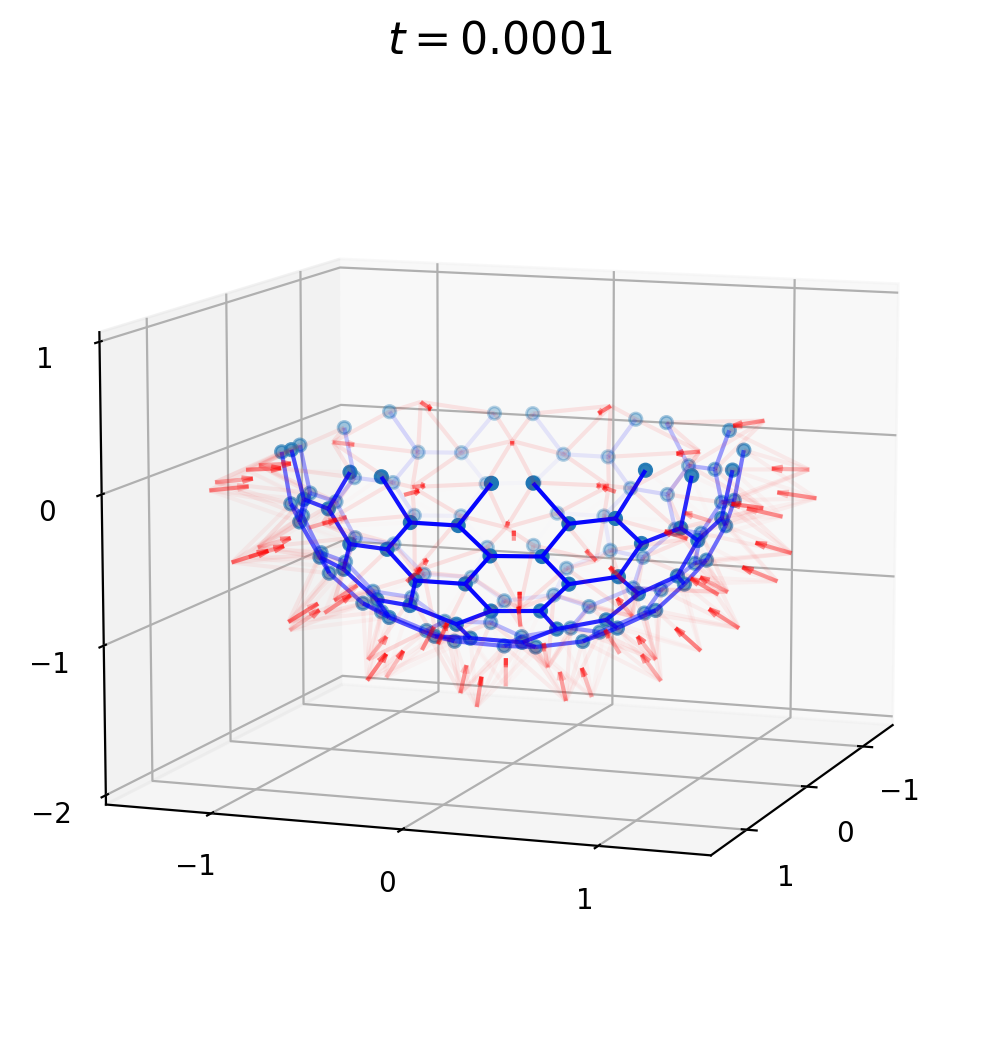
\includegraphics[width=0.4\textheight]{dynamics/00000.png}
	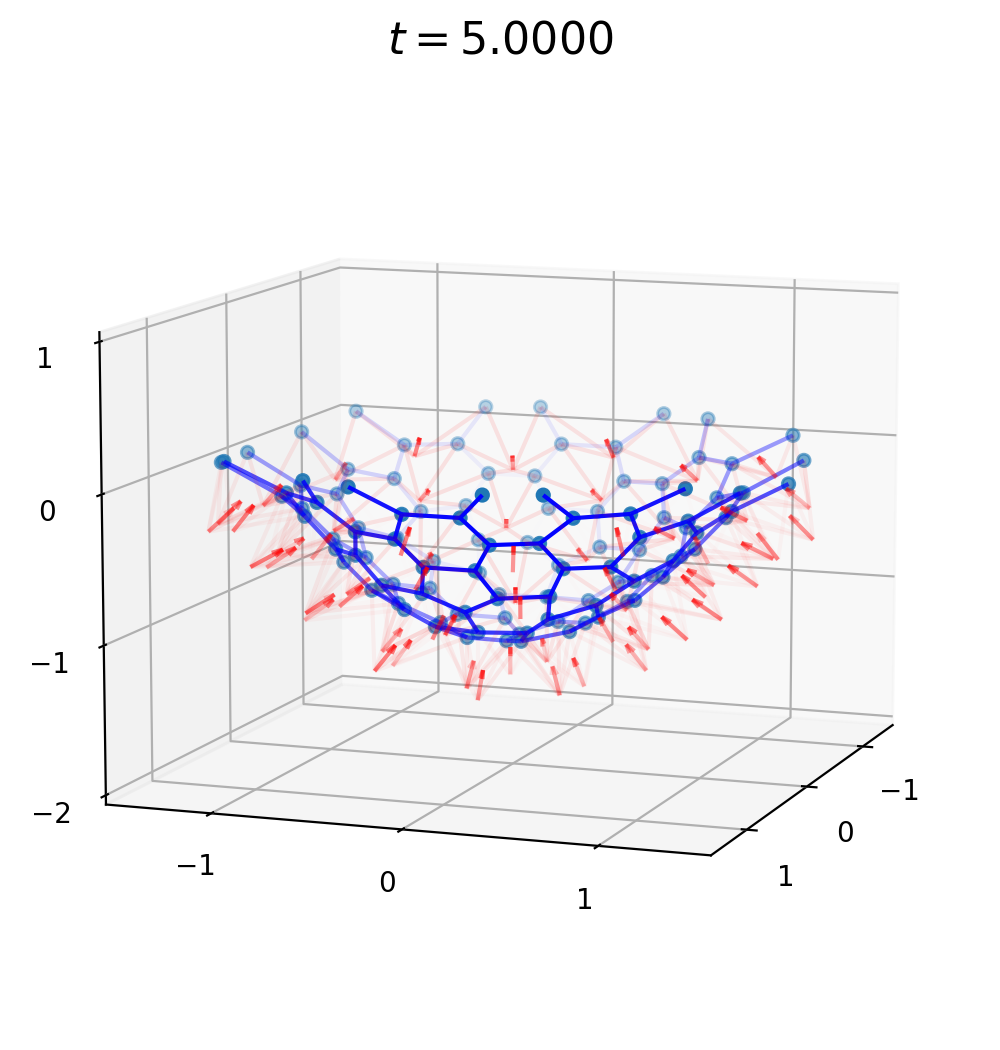
\includegraphics[width=0.4\textheight]{dynamics/02000.png}
	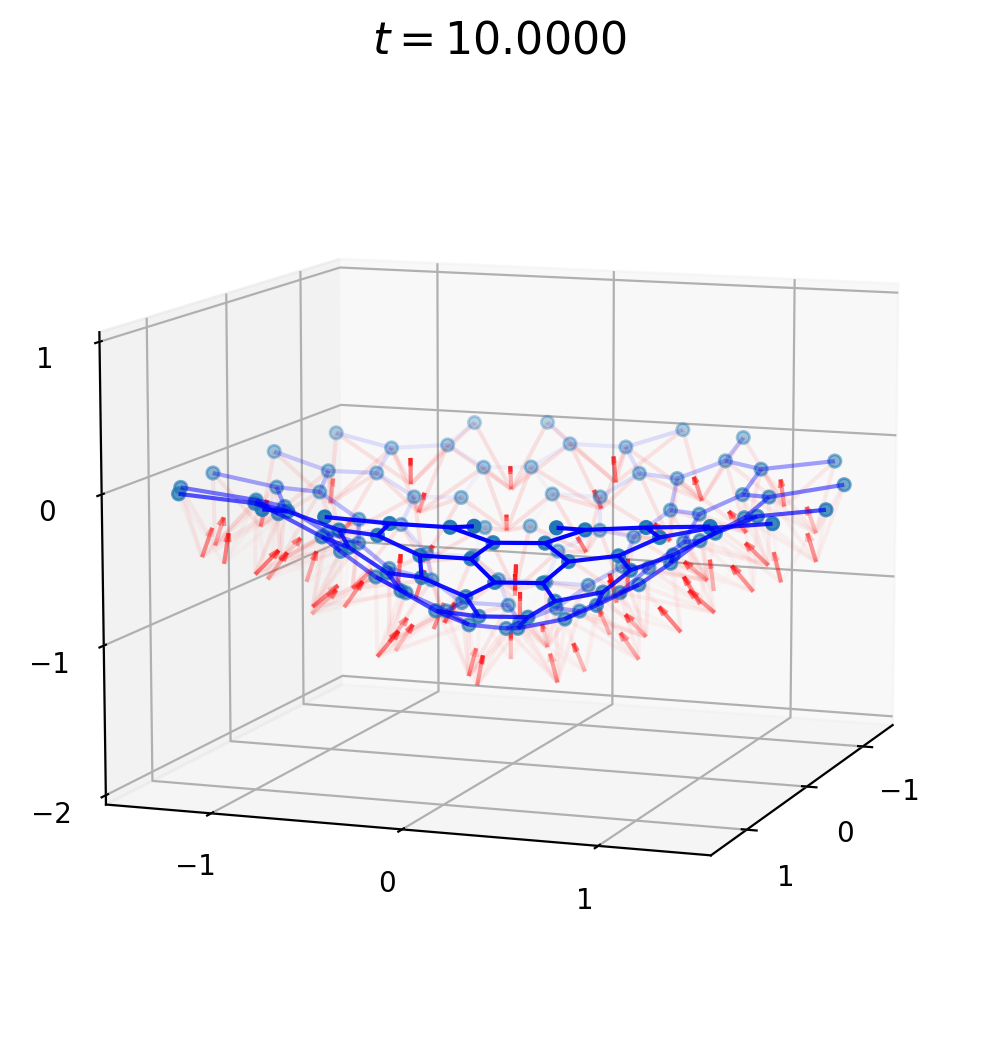
\includegraphics[width=0.4\textheight]{dynamics/04000.png}
	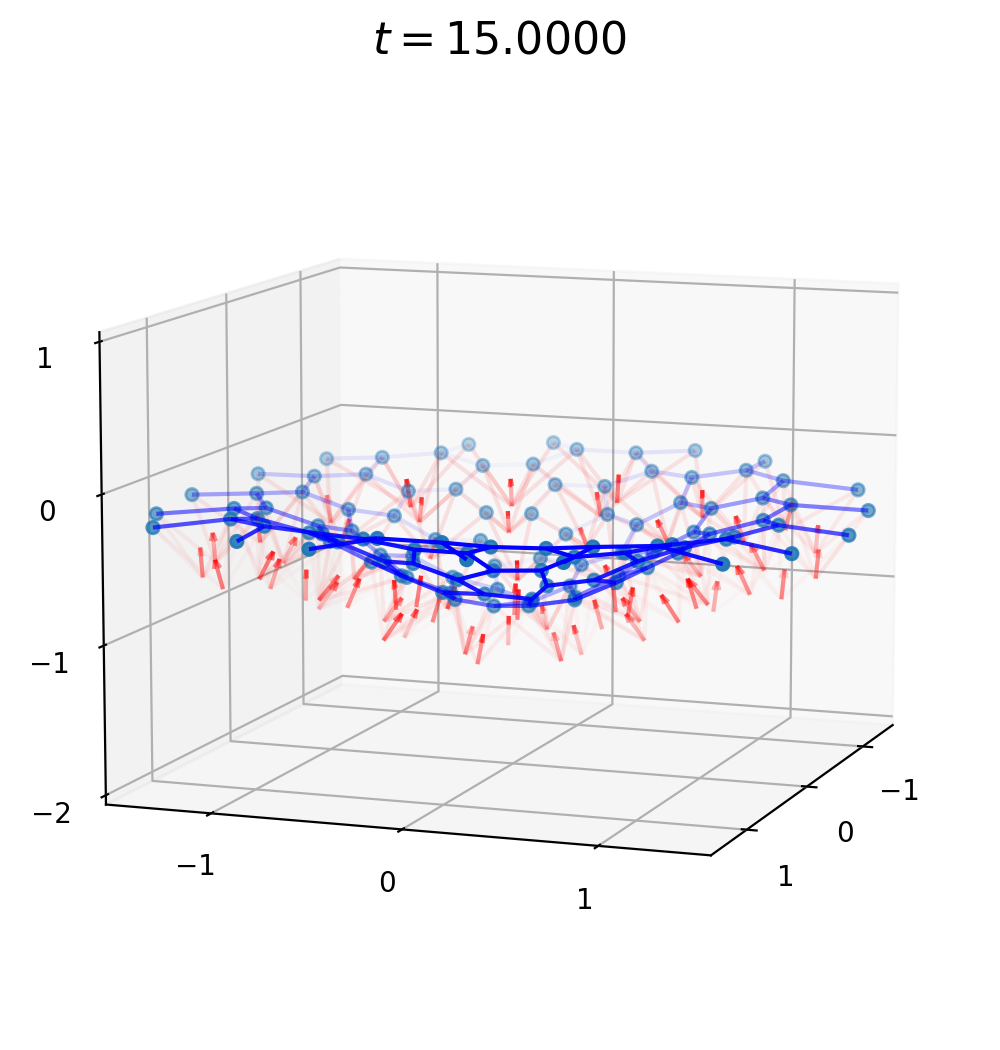
\includegraphics[width=0.4\textheight]{dynamics/06000.png}
	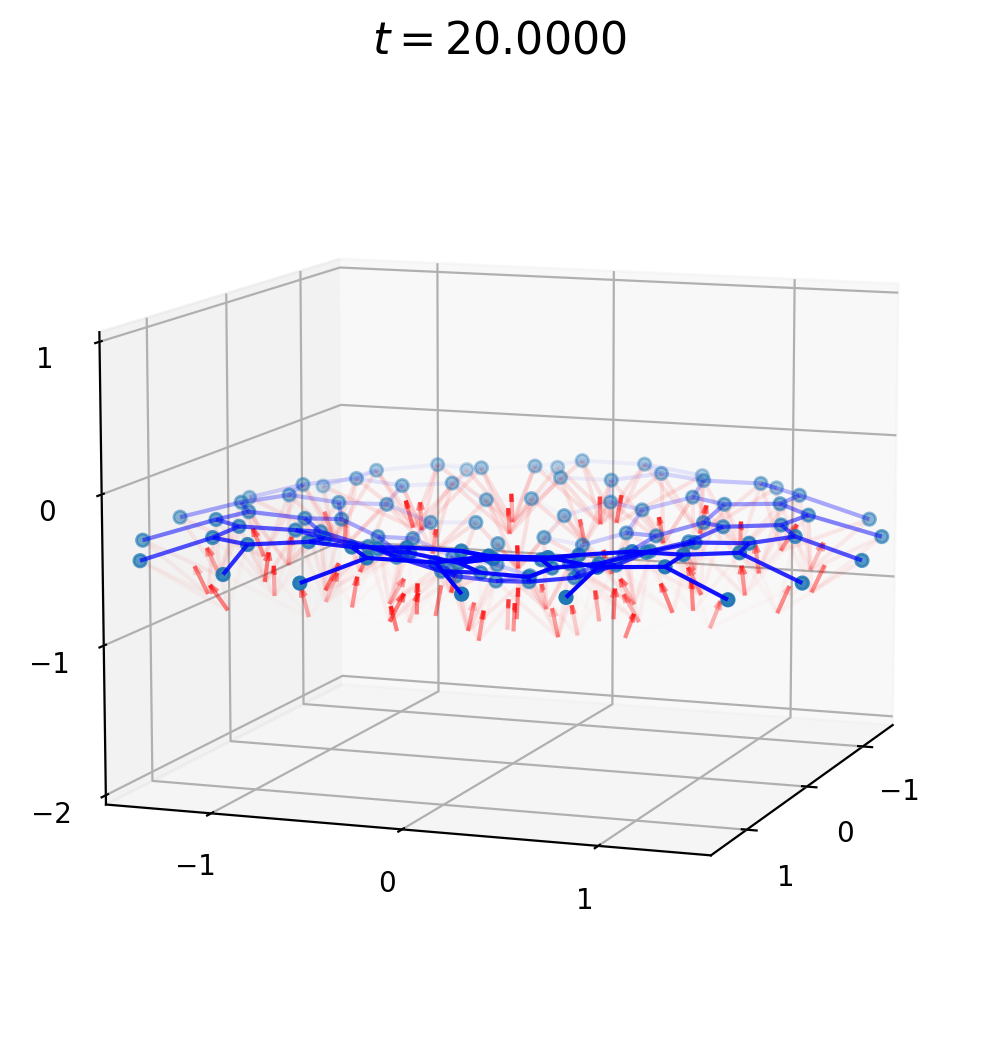
\includegraphics[width=0.4\textheight]{dynamics/08000.png}
	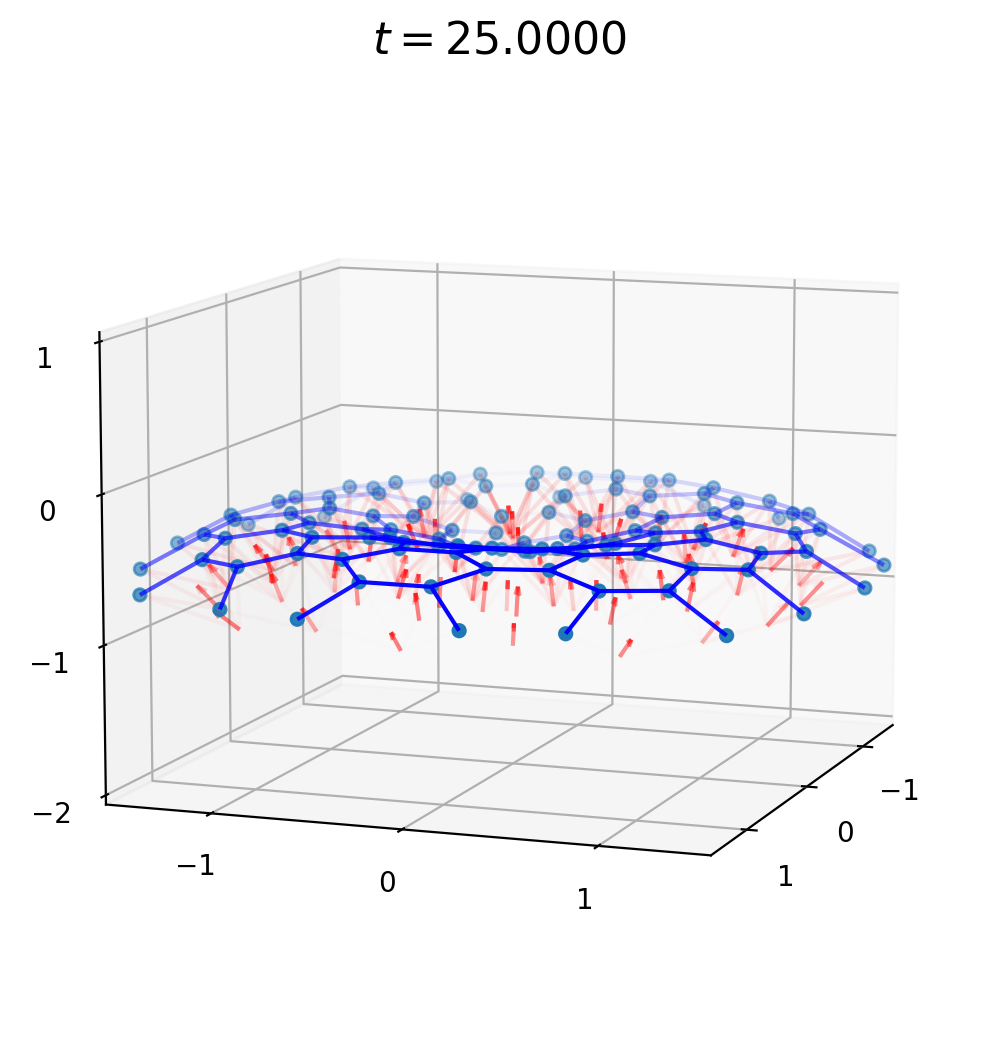
\includegraphics[width=0.4\textheight]{dynamics/10000.png}
	\caption[Gradient descent equilibration and dynamics of sheet inversion]{Dynamics of sheet inversion under linear drag in the transition from $(\phi_0, \psi_0)=(0.55, 0.65)$ to $(0.71,0.41)$ demonstrating projected gradient descent using \cref{eq:grad_desc_r,eq:grad_desc_n1,eq:grad_desc_n2}.}
	\label{fig:dynamics}
\end{figure}
\end{landscape}

While the forward integration works well for small sheets with simple graph topologies, I found that some equilbrium angles $\phi_0, \psi_0$ caused some sheets to strain to such an extreme that collar vertices would cross through each other. 
The resulting increase in energy comes from the discontinuous sign function in the definition of $\psi$ (\cref{eq:psi}), and collar vertices cross over each other due to too large of a step size $\Delta t$. 
While adaptively decreasing the step size is a viable option, it would substantially slow the equilibration algorithm.  
Instead, I introduced an additional term to the energy $\e_\varphi$ based on the angles $\varphi_{\rho\alpha\sigma}$ formed by each cell $\alpha$ and its adjacent pairs of collar vertices $\rho,\sigma$ when projected onto the plane defined by the cell normal $\bh{n}_\alpha$ (\cref{fig:varphi}):
\begin{align}
	\e_\varphi &= k_\varphi \sum_{(\alpha,\beta:\rho\sigma)} \left(\varphi_{\rho\alpha\sigma} - \varphi_{0\rho\alpha\sigma} \right)^2, \label{eq:e_varphi}
\end{align}
\noindent where $\varphi_{0\rho\alpha\sigma}$ is an equilibrium projected collar-cell-collar angle for each triple. 
Each angle $\varphi_{0\rho\alpha\sigma}$ is set to the actual value that is evaluated at the initial sheet geometry.
Unless specified otherwise, the constant $k_\varphi$ is set to $0.3k_\phi$, which was qualitatively found to be a reasonable balance between preventing numerical instability and minimally interfering in the structure transition.
It is worth noting that $\e_\varphi$ has physical interpretation as penalising collars that do not extend radially outward relative to the cell's normal vector.

\begin{figure}
	\centering 
	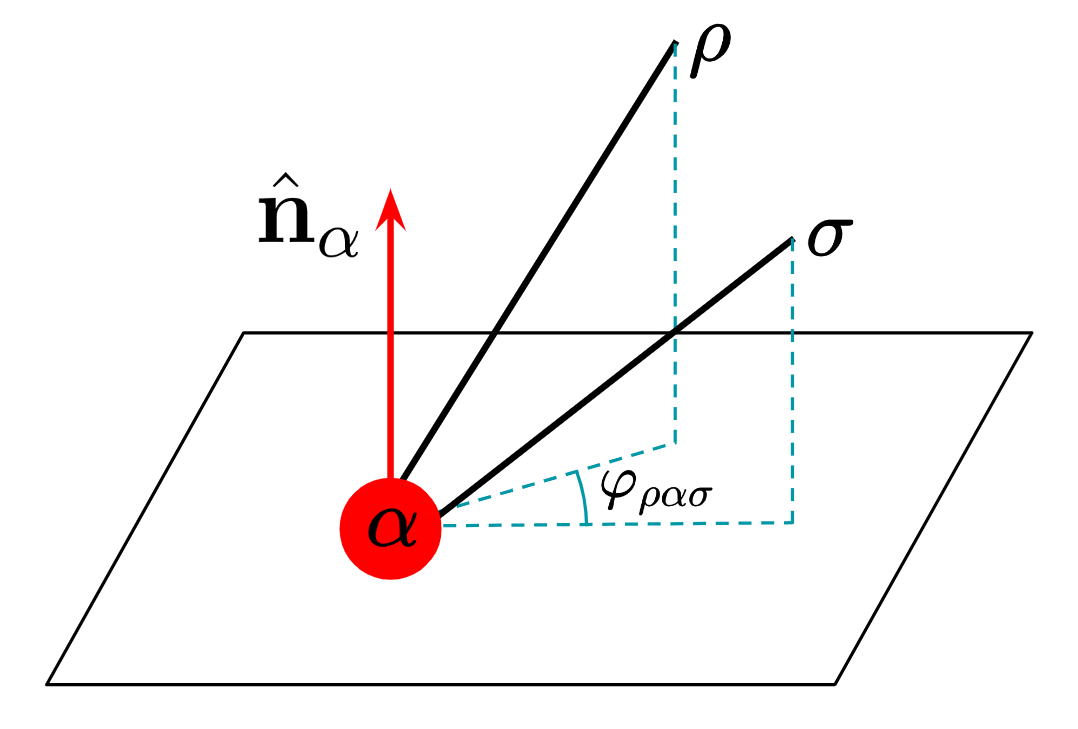
\includegraphics[width=0.5\textwidth]{varphi.png}
	\caption{Geometry for calculating $\varphi_{\rho\alpha\sigma}$.}
	\label{fig:varphi}
\end{figure}

The angles $\varphi_{\rho\alpha\sigma}$ are calculated similarly to $\phi, \psi$ (\cref{eq:phi,eq:psi}),
\begin{align}
	\varphi_{\rho\alpha\sigma} &= \arccos \left[\vec{\alpha\rho}_\| \cdot \vec{\alpha\sigma}_\| \right], \label{eq:varphi}
\end{align}
\noindent where $\vec{\alpha\rho}_\|$ is the projection of $\vec{\alpha\rho}$ onto the plane defined by normal $\bh{n}_\alpha$ and position $\bm{r}_\alpha$:
\begin{align*}
\vec{\alpha\rho}_{\|} &= \vec{\alpha\rho} - (\vec{\alpha\rho} \cdot \bh{n}_\alpha) \bh{n}_\alpha.
\end{align*}

% The gradient of $\e_\varphi$ is given by 
% 
% \begin{align}
% 	todo \label{eq:grad_varphi}
% \end{align}

Note that 
\begin{align}
	\bm{0} &= \sum_\gamma \frac{\partial}{\partial\bm{r}_\gamma} \e \label{eq:force_zero}
\end{align}
since all forces are generated internally.
Moveover, \cref{eq:force_zero} holds individually for each term in the energy (\cref{eq:e}), which is evident by the indicator functions in \cref{eq:grad_phi,eq:grad_psi,eq:grad_sp}.

\subsection{Exploring the energy landscape} \label{subsec:landscape}

With the ability to study discrete sheet equilibrium geometries and dynamics, we are prepared to evaluate a mechanism for \textit{C. flexa} folding and inversion. 
Based on the two collar angle states observed in \citet{brunet2019}, a reasonable model would be to assume relaxed-state equilibrium angles $\phi_{\text{in}}, \psi_{\text{in}}$ and a different set of active-state angles $\phi_{\text{out}}, \psi_{\text{out}}$ with instantaneous transition between the two states. 
The rapid change in individual cell behavior and expected gradual sheet shape change expected from opposing cell-cell interactions align with our expectations from observations \citet{brunet2019}. 

Although we cannot access true values for the equilibrium angles, modeling \textit{C. flexa} sheets numerically provides the opportunity to explore the entire energy landscape. 
For sheets generated with a regular hexagonal lattice, we observe the expected diagonal valley where energy in minimised in the energy landscape since the sheet is expected to be flat along those pairs $(\phi_0, \psi_0)$ (\cref{fig:landscape_flat}) (\cref{subsubsec:flat}).
Substantial sheet deformation and bending is evidently not sufficient to overcome the change in terms in the energy function. 
The increases in energy when the equilibrium angles are most disparate can be interpreted as collar microvilli stretching or compressing to accommodate sheet bending or a difference in the bending at each cell from the preferred state. 
For example, cells at either the centre nor boundary in a bent sheet (\cref{fig:landscape_flat}, bottom-right or top-left) must contribute a positive contribution to $\e$ since they do not have the symmetric bending at all collar microvilli prescribed by \cref{eq:e_phi,eq:e_psi,eq:e_sp}.

\begin{figure}
	\centering
	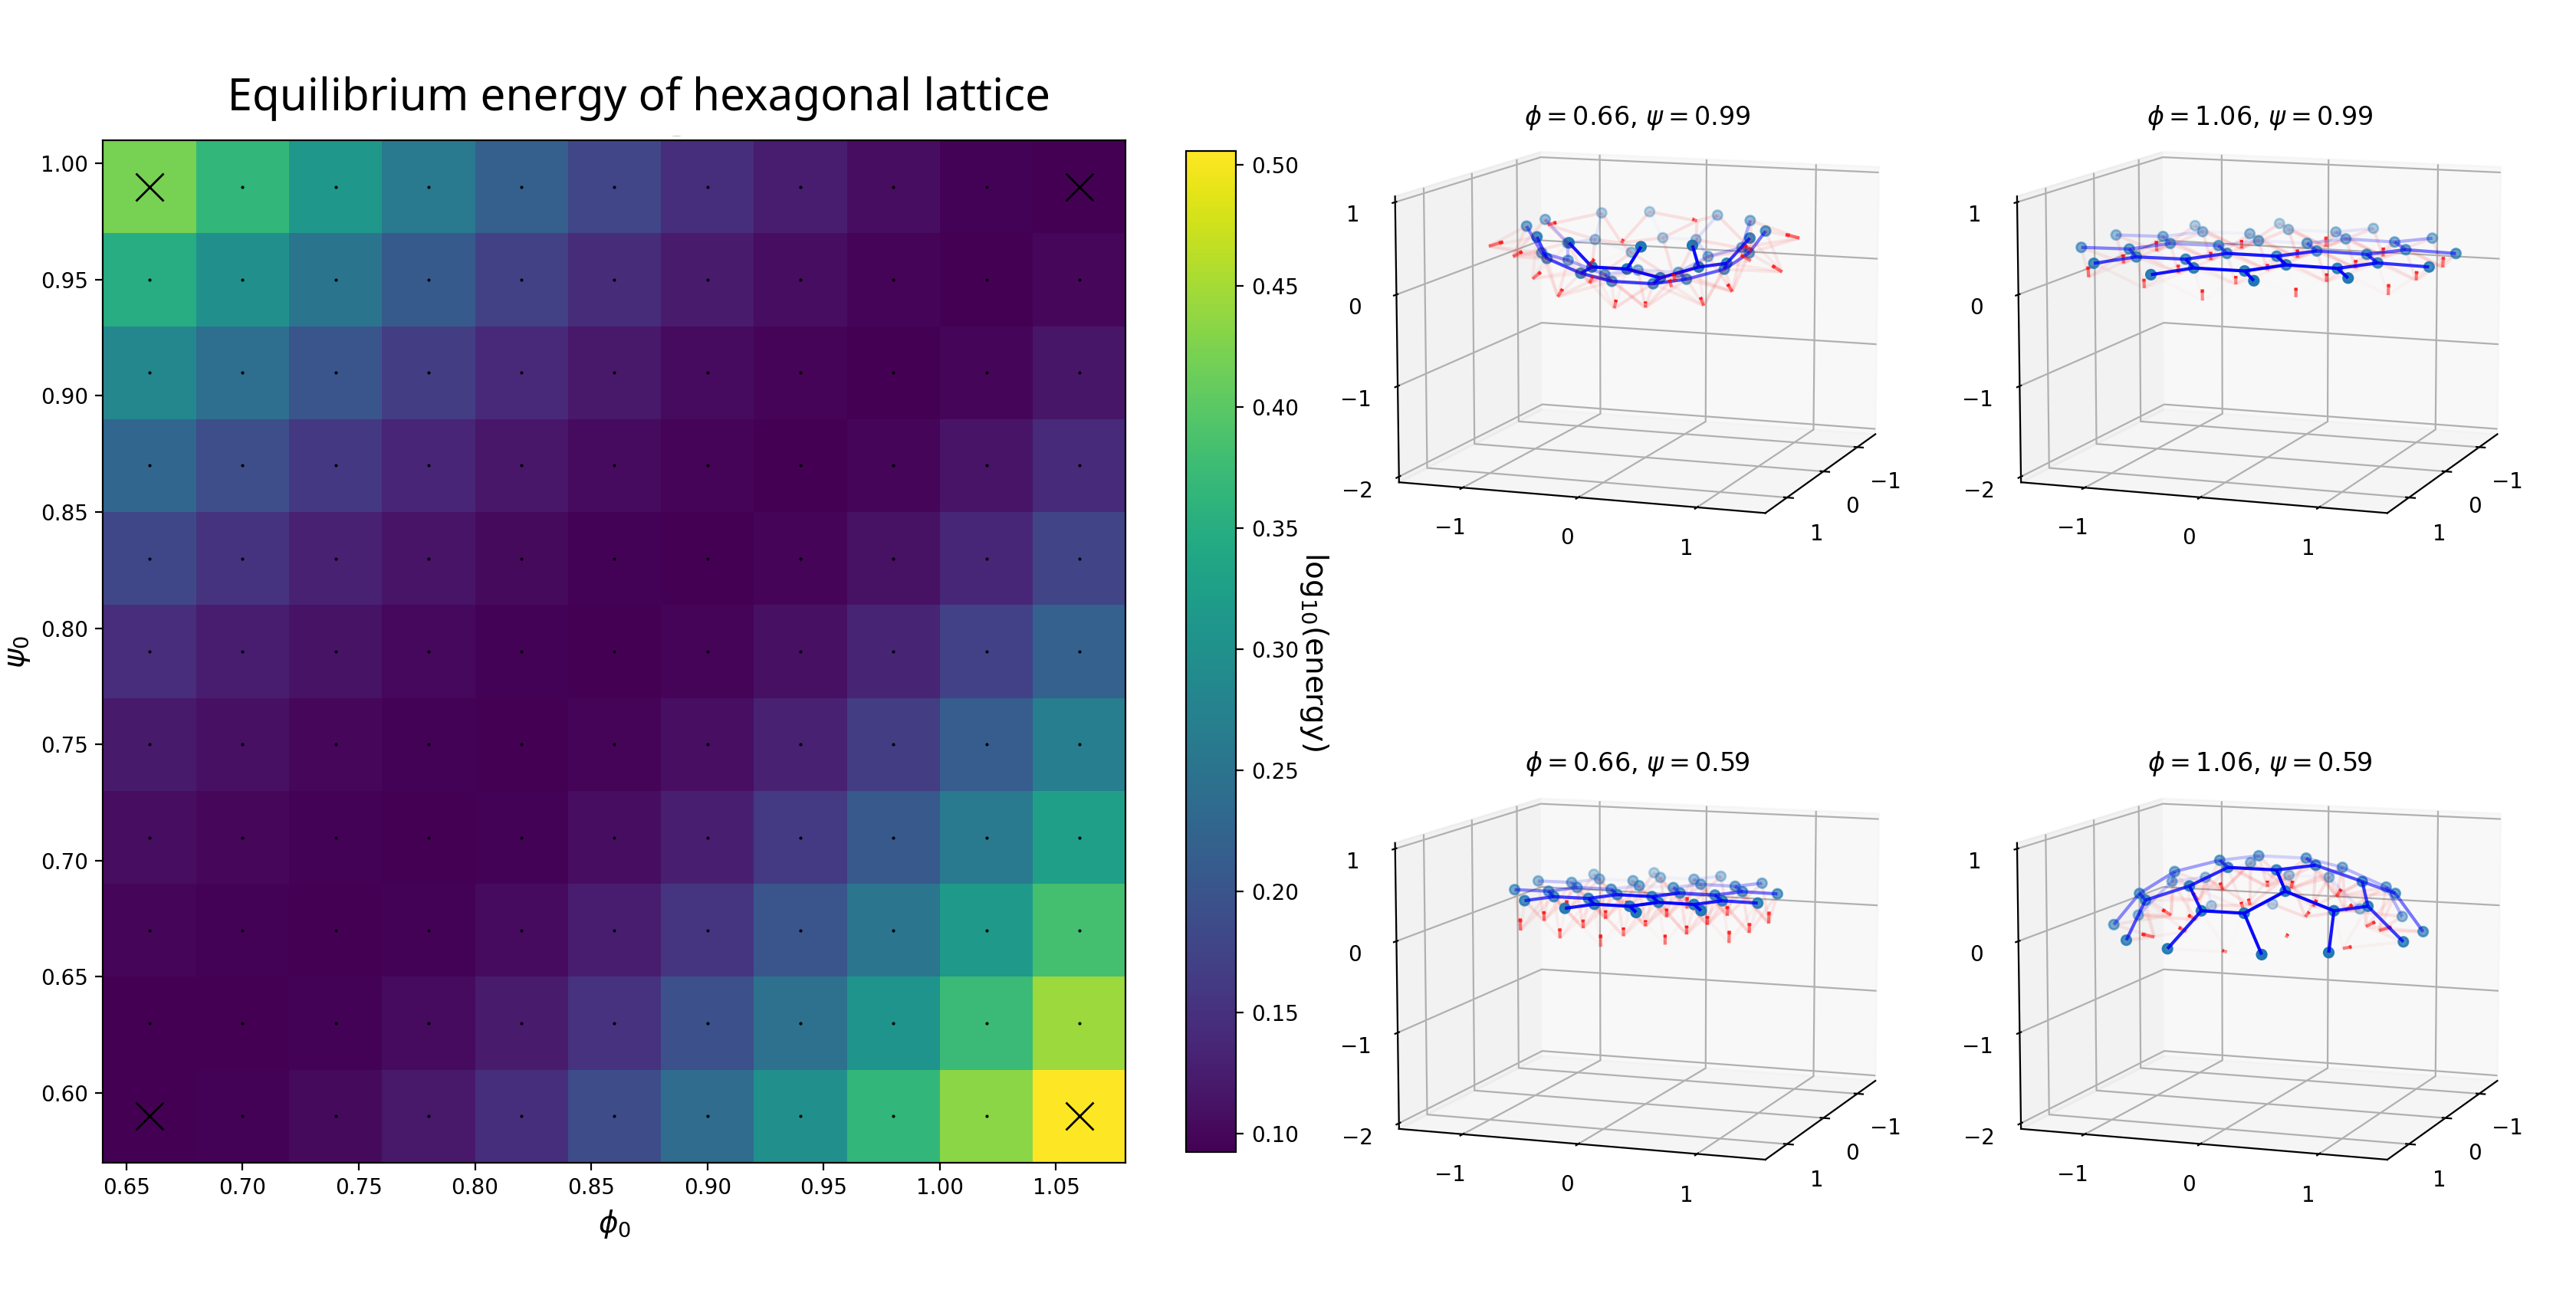
\includegraphics[width=\textwidth]{landscape_hex.png}
	\caption[Energy landscape of a discrete \textit{C. flexa} sheet generated from a hexagonal lattice]{Energy landcsape of a discrete \textit{C. flexa} sheet generated from a hexagonal lattice. Sheets displayed at the right correspond to the corners of the landscape indicated with white crosses. Energy along the diagonal is slightly above zero due to finite termination of gradient descent.}
	\label{fig:landscape_flat}
\end{figure}

We can observe a more rich energy landscape by using a graph topology containing defects from a hexagonal lattice.
A simple choice is an icosahedron, which is formed using a polyhedron of twelve vertices each of degree five forming twenty faces of equilateral triangles.
Each triangular face can each be repeatedly subdivided into four smaller equilateral triangular face by introducing a vertex along each edge, such that the surface gains vertices of degree six in a hexagonal lattice \citep{dahl2014}.
Intuitively, the fixed number of vertices with degree five make it possible for the vertices to form a closed surface.
For example, the patchwork of a football is formed by replacing each degree-five vertex of an icosahedron with a regular pentagon, and the polygons on the surface are able to form a regular pattern while forming an overall curved surface due to the diversity of shapes present.
The edges of a small section of the icosphere with two subdivisions are shown in blue at the collar-collar interfaces in \cref{fig:landscape_ico}, and edges for larger sections of the icosphere are shown in \cref{fig:landscape_ico3,fig:landscape_ico4}.

A flexa sheet with collar-collar boundaries defined along a small section of the icosphere gives an energy landscape with two diagonal valleys corresponding to flagella-in and flagella-out sheets (upper and lower, respectively) in \cref{fig:landscape_ico}.
That there are two valleys, rather than the one valley along $\phi_0 = \psi_0$, is interpreted to be the result of topological defects in the lattice structure that are essential to the construction of the icosphere. 
The two energy valleys achieve similar values for the minimum sheet energy, suggesting there is not necessarily any energetic preference to either state in this model.
The positive and negative sheet curvatures respectively, in the convention of \cref{ch:2} is consistent with how we expect $\phi_0$ and $\psi_0$ to induce spontaneous curvature (\cref{eq:h0}).
The continuity between the two valleys indicates that sheets are stably able to flatten and the minimum energy structures continuously transition between flagella-in and -out structures. 
The landscape was found to differ negligibly when an inverted sheet was used to initialise the simulations.

\begin{figure}[hbtp]
	\centering
	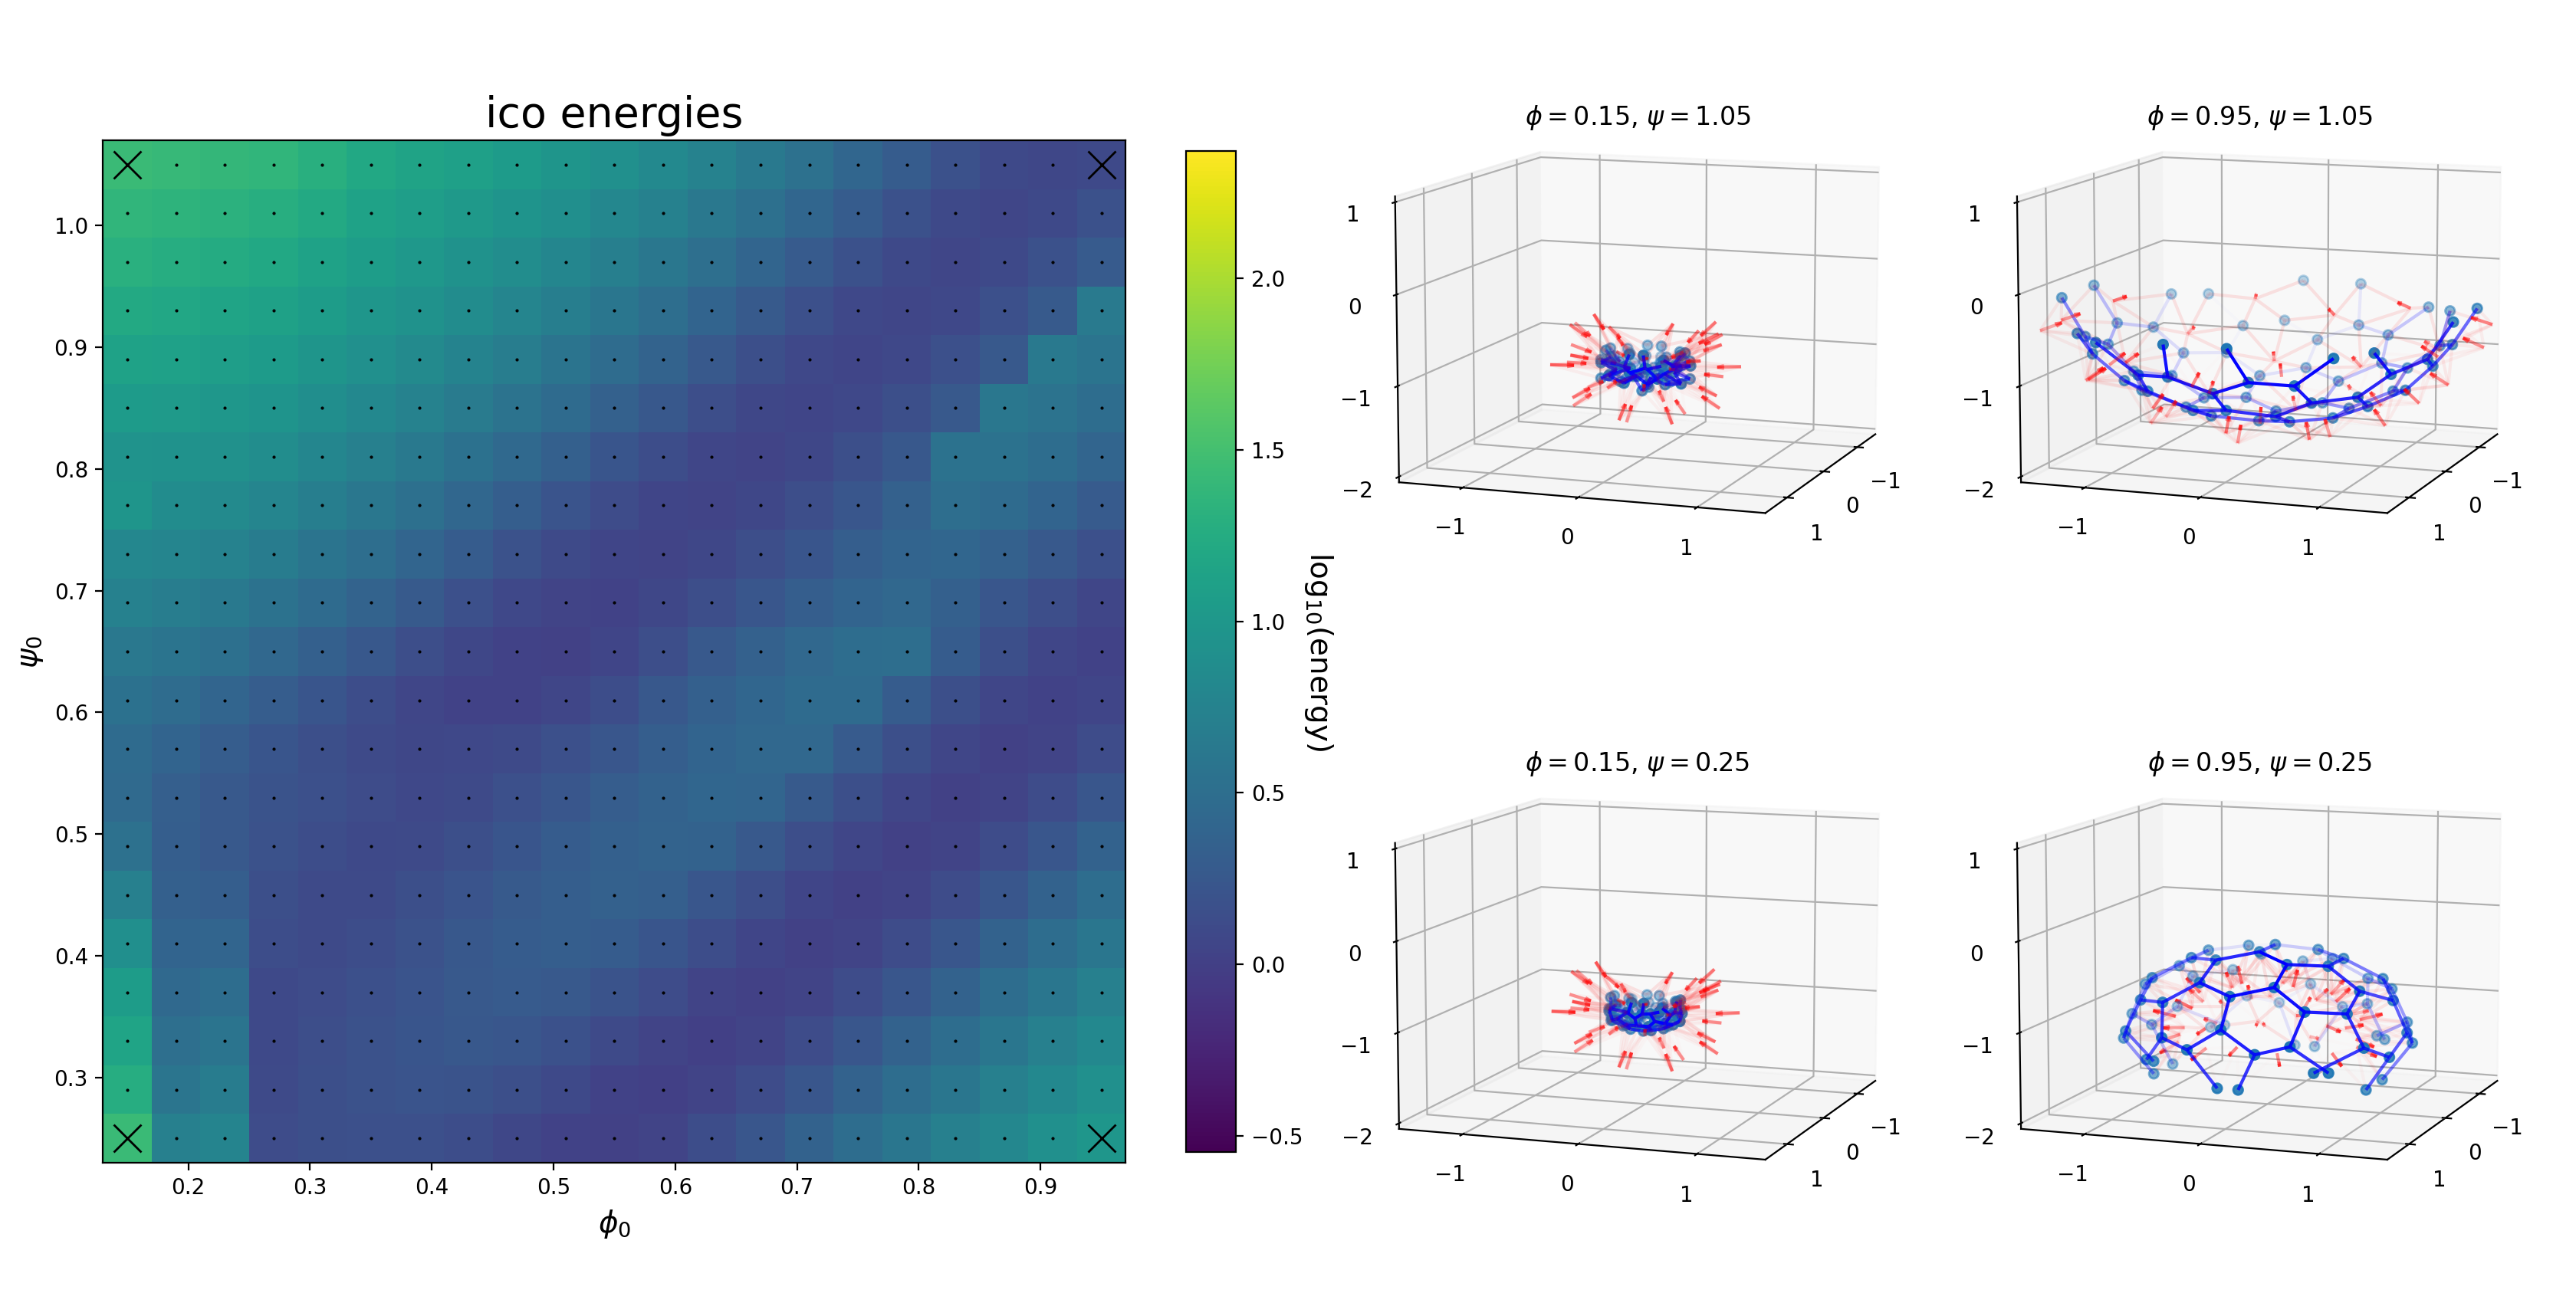
\includegraphics[width=\textwidth]{landscape_ico.png}
	\caption[Energy landscape of a discrete \textit{C. flexa} sheet generated from a small icosphere section]{Energy landscape of a discrete \textit{C. flexa} sheet generated from a thrice-subdivided icosphere section. Style as in \cref{fig:landscape_flat}. The icosphere was generated using code from \citep{dahl2014}. Cells comprising topological defects (those with five neighbours instead of the typical six) can be seen in the bottom-right-most panel, at the top right of the sheet and at the top left. The latter is difficult to see because the cell-cell collar interface boundaries (translucent blue points) are nearly collinear in the projection used to plot the sheet.}
	\label{fig:landscape_ico}
\end{figure}

\subsection{Sudden inversion}

Adding more cells by taking more vertices from the icosphere (with polar angle at least $2\pi/5$) again produces two energy valleys corresponding to flagella-in and -out sheets (\cref{fig:landscape_ico3}). 
In a larger sheet, however, we identify a discontinuity when beginning from a flagella-in sheet and changing parameters to achieve inversion (\cref{subfig:landscape_ico3}) as in \cref{fig:dynamics}.
The discontinuity implies that equilibrated sheets flagella-in sheets there achieve a local energy minimum, but that a global minimum may be achieved instead by taking a flagella-out sheet with the same parameters. 
Indeed, when using flagella-out sheets as initial conditions, the complete flagella-out energy valley is apparent and the discontinuity shifts to show the flagella-out to -in transition (\cref{subfig:landscape_ico3r}).\footnote{The large vertical discontinuity along $\phi_0=0.41$ is a consequence of the simulation parallelisation. All landscape plots shown were simulated by first equilibrating at the landscape centre ($\phi_0=0.55,\psi_0=0.65$). The row $\psi_0=0.65$ was simulated by using this as an initial condition to consecutively equilibrate to a larger or smaller value of $\phi_0$. Sheets were then simulated in columns from the central row for increasing or decreasing $\psi_0$. The vertical discontinuity indicates where the initial row simulations first transitioned, such that the sheets with $\phi_0=0.39$ in \cref{subfig:landscape_ico3r} began with a flagella-in sheet.}
Note that the sheet geometries at the landscape corners in \cref{fig:landscape_ico3} are the same, confirming inversion and the existence of unique minima in the landscape.

\begin{figure}
	\centering
	\begin{subfigure}[b]{\textwidth}
		\centering
		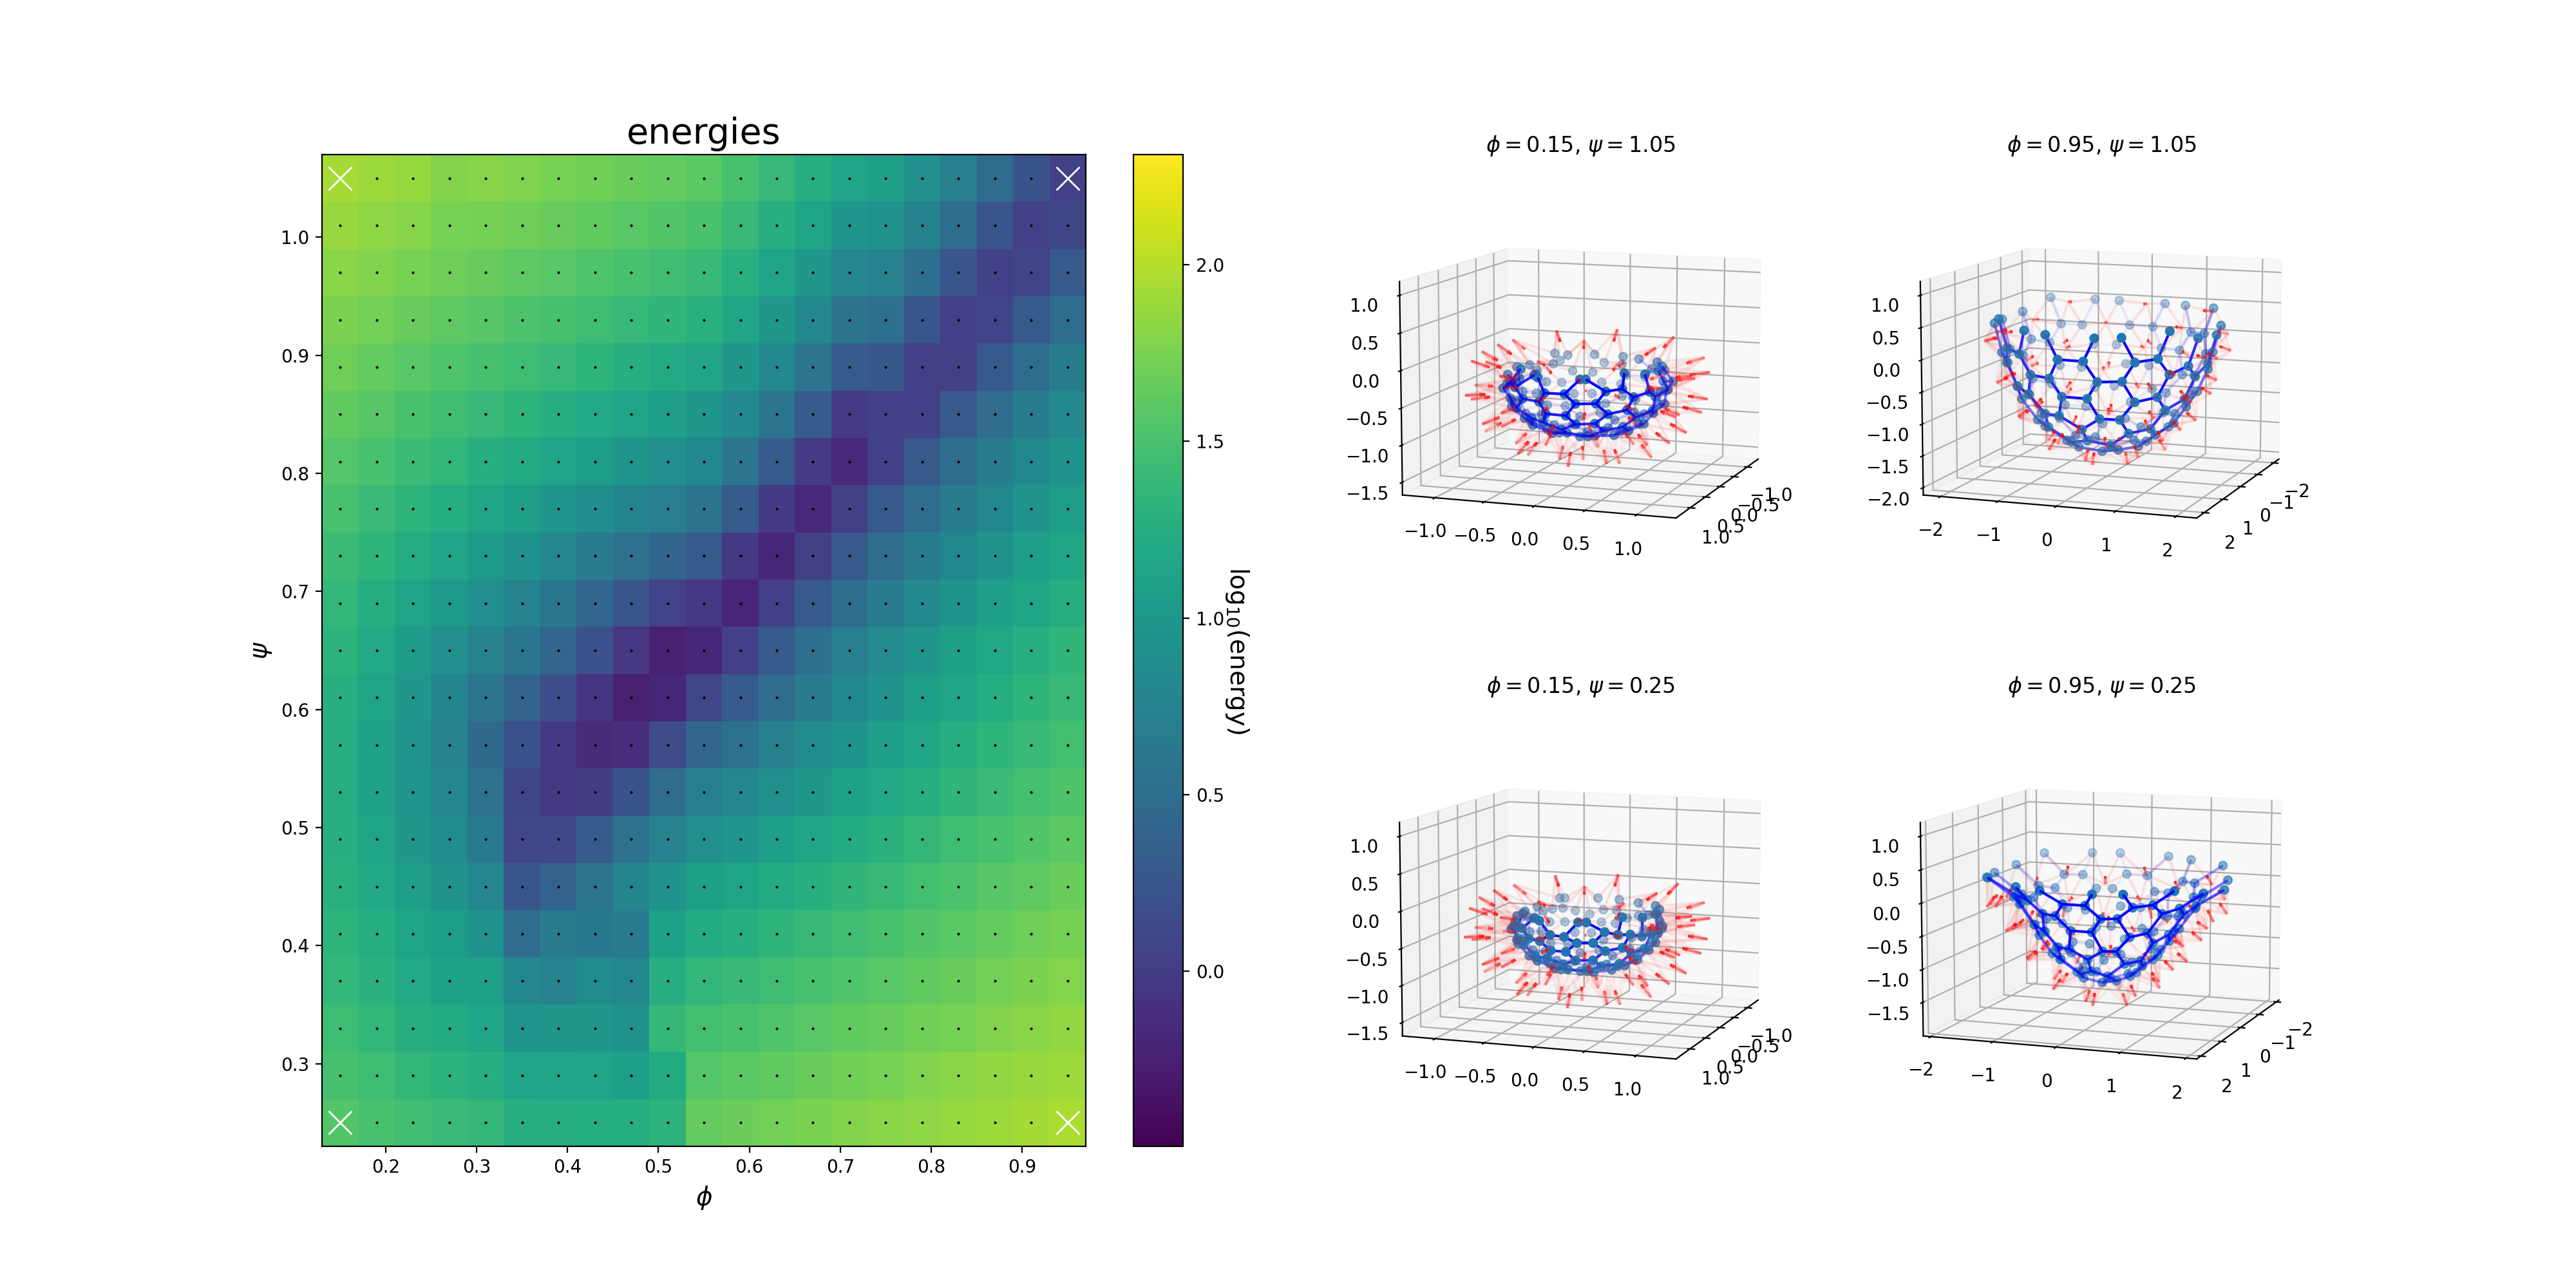
\includegraphics[width=\textwidth]{landscape_ico3.png}
		\caption{}
		\label{subfig:landscape_ico3}
	\end{subfigure}
	\begin{subfigure}[b]{\textwidth}
		\centering
		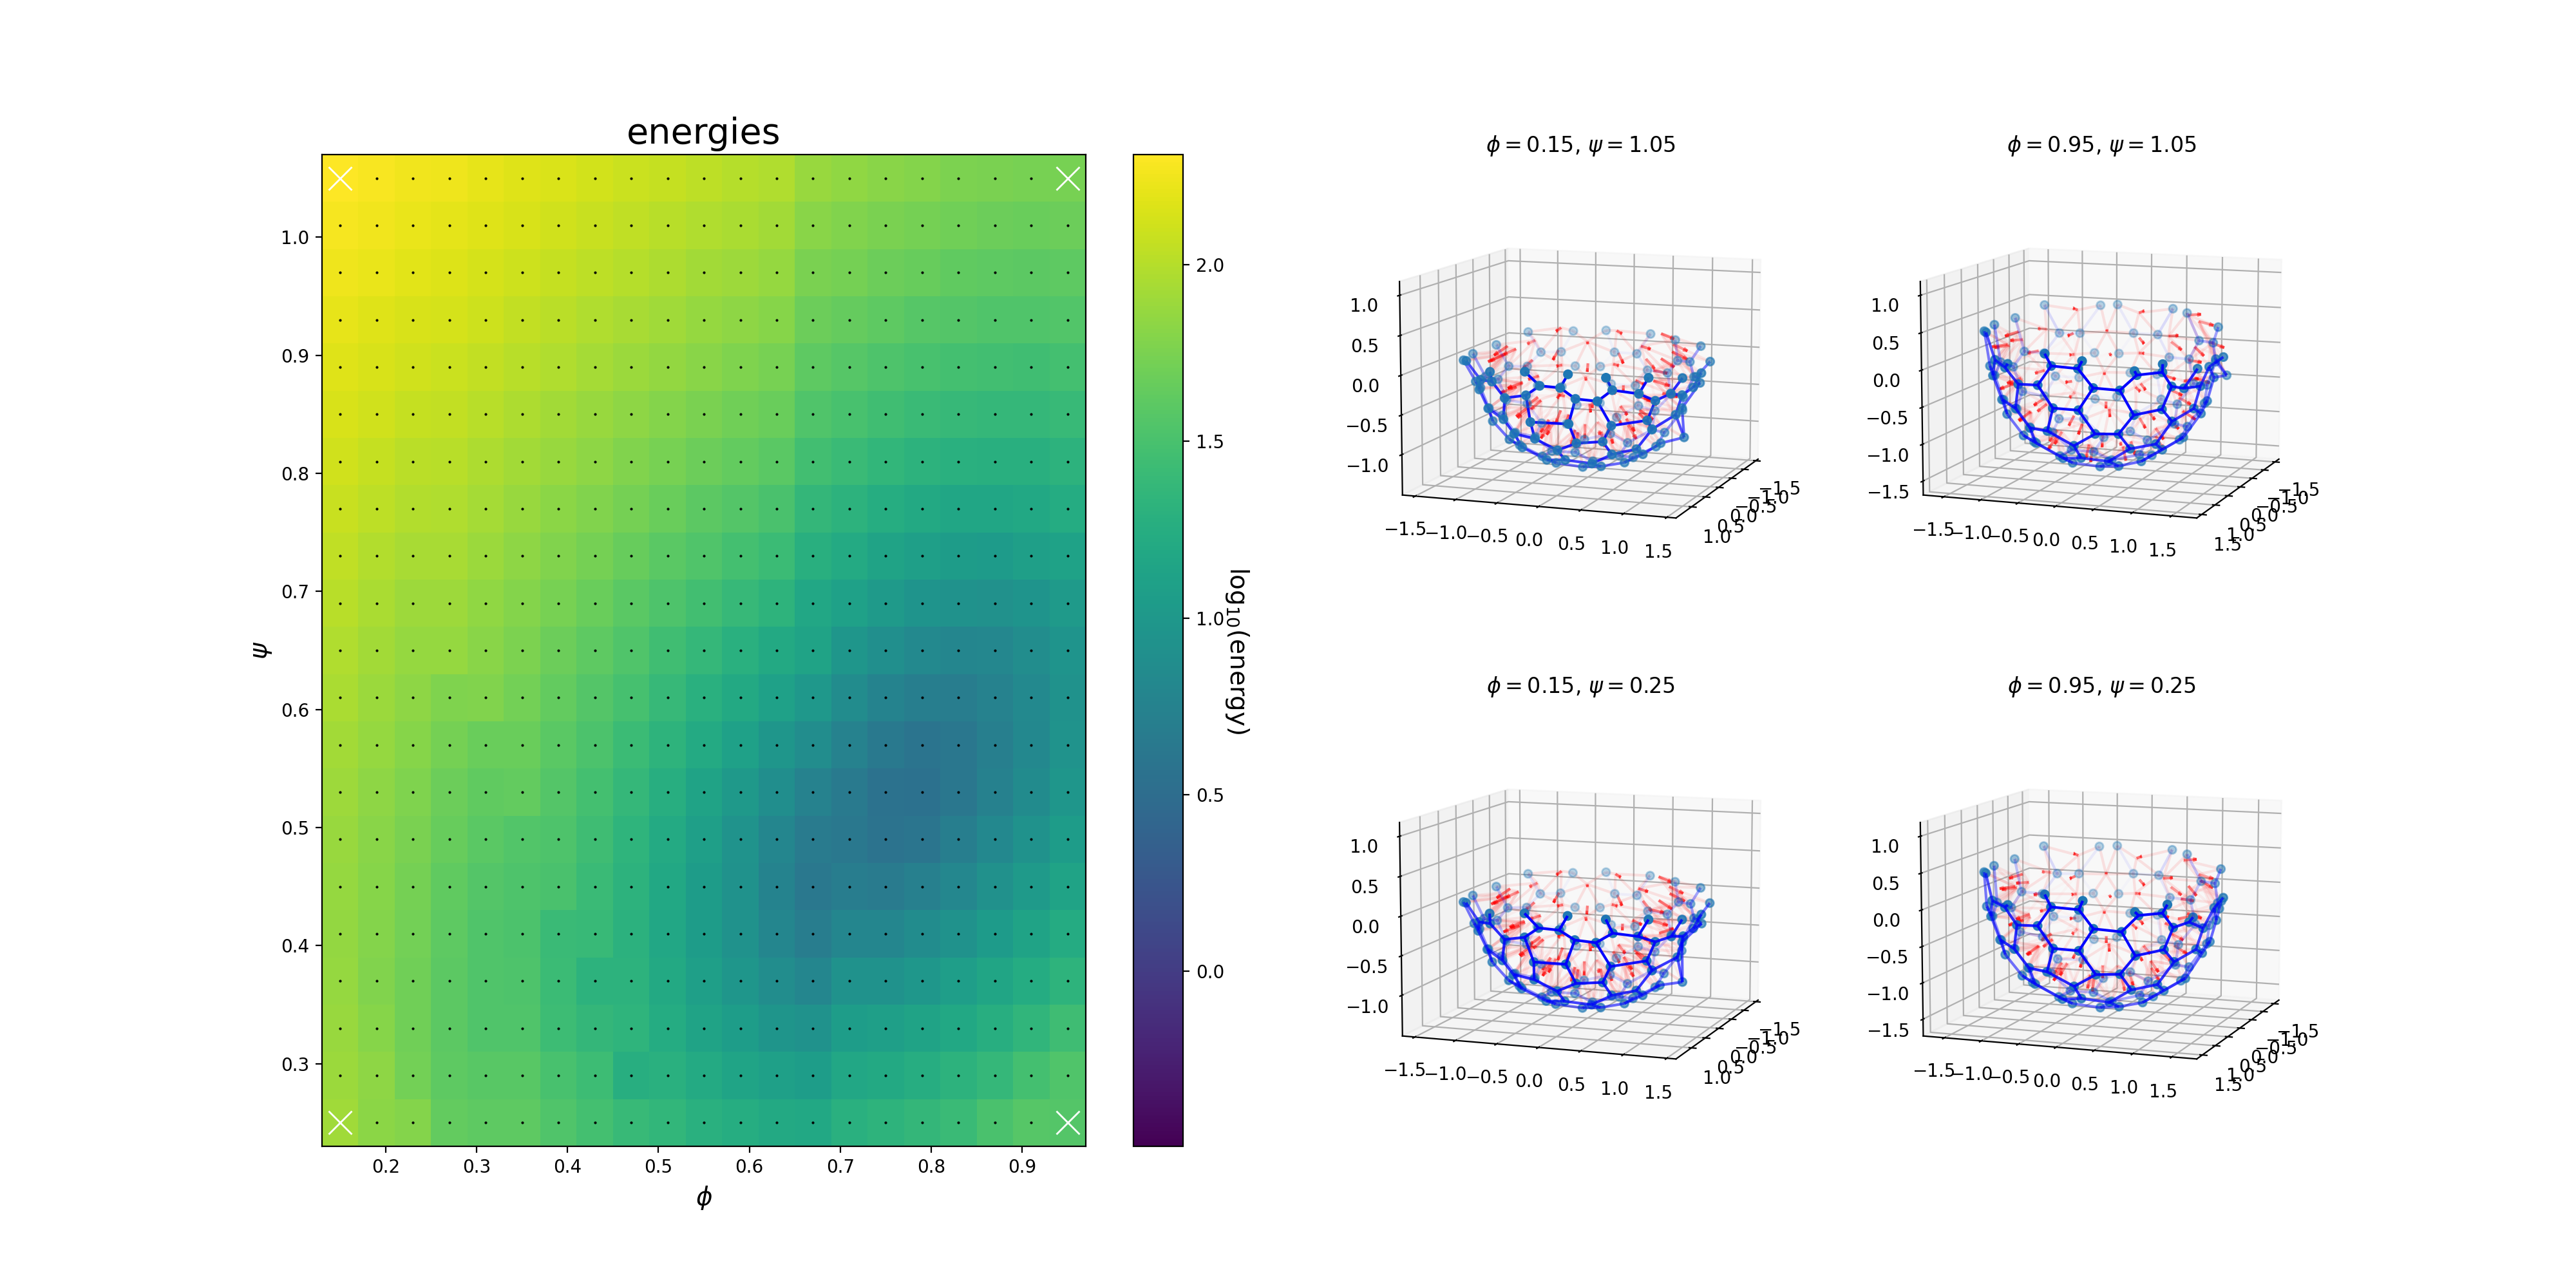
\includegraphics[width=\textwidth]{landscape_ico3r.png}
		\caption{}
		\label{subfig:landscape_ico3r}
	\end{subfigure}
	\caption[Energy landscape for flagella-in and flagella-out curved sheets]{Energy landscapes for (\ref{subfig:landscape_ico3}) flagella-in and (\ref{subfig:landscape_ico3r}) flagella-out sheets of \textit{C. flexa}. The color scaling is the same in both images. The landscapes for a smaller segment of the icosphere were qualitatively similar. Cells with five neighbours are easily visible in the bottom-right-most panel of \ref{subfig:landscape_ico3}, where one such cell is visible in the foreground and another is visible at the top right of the image.}
	\label{fig:landscape_ico3}
\end{figure}

As we are interested in the bistability and transition in \textit{C. flexa} sheets, we are concerned with the global energy minima for both flagella-in and -out sheets. 
In \cref{fig:landscape_merge}, the minimum energy geometries from the landscapes of \cref{fig:landscape_ico3} are shown with an indication which of the two plots the conformation came from.
The gloabl energy minima show two clear contiguous minimum energy valleys, as in \cref{fig:landscape_ico}.

\begin{figure}[ptbh]
	\centering
	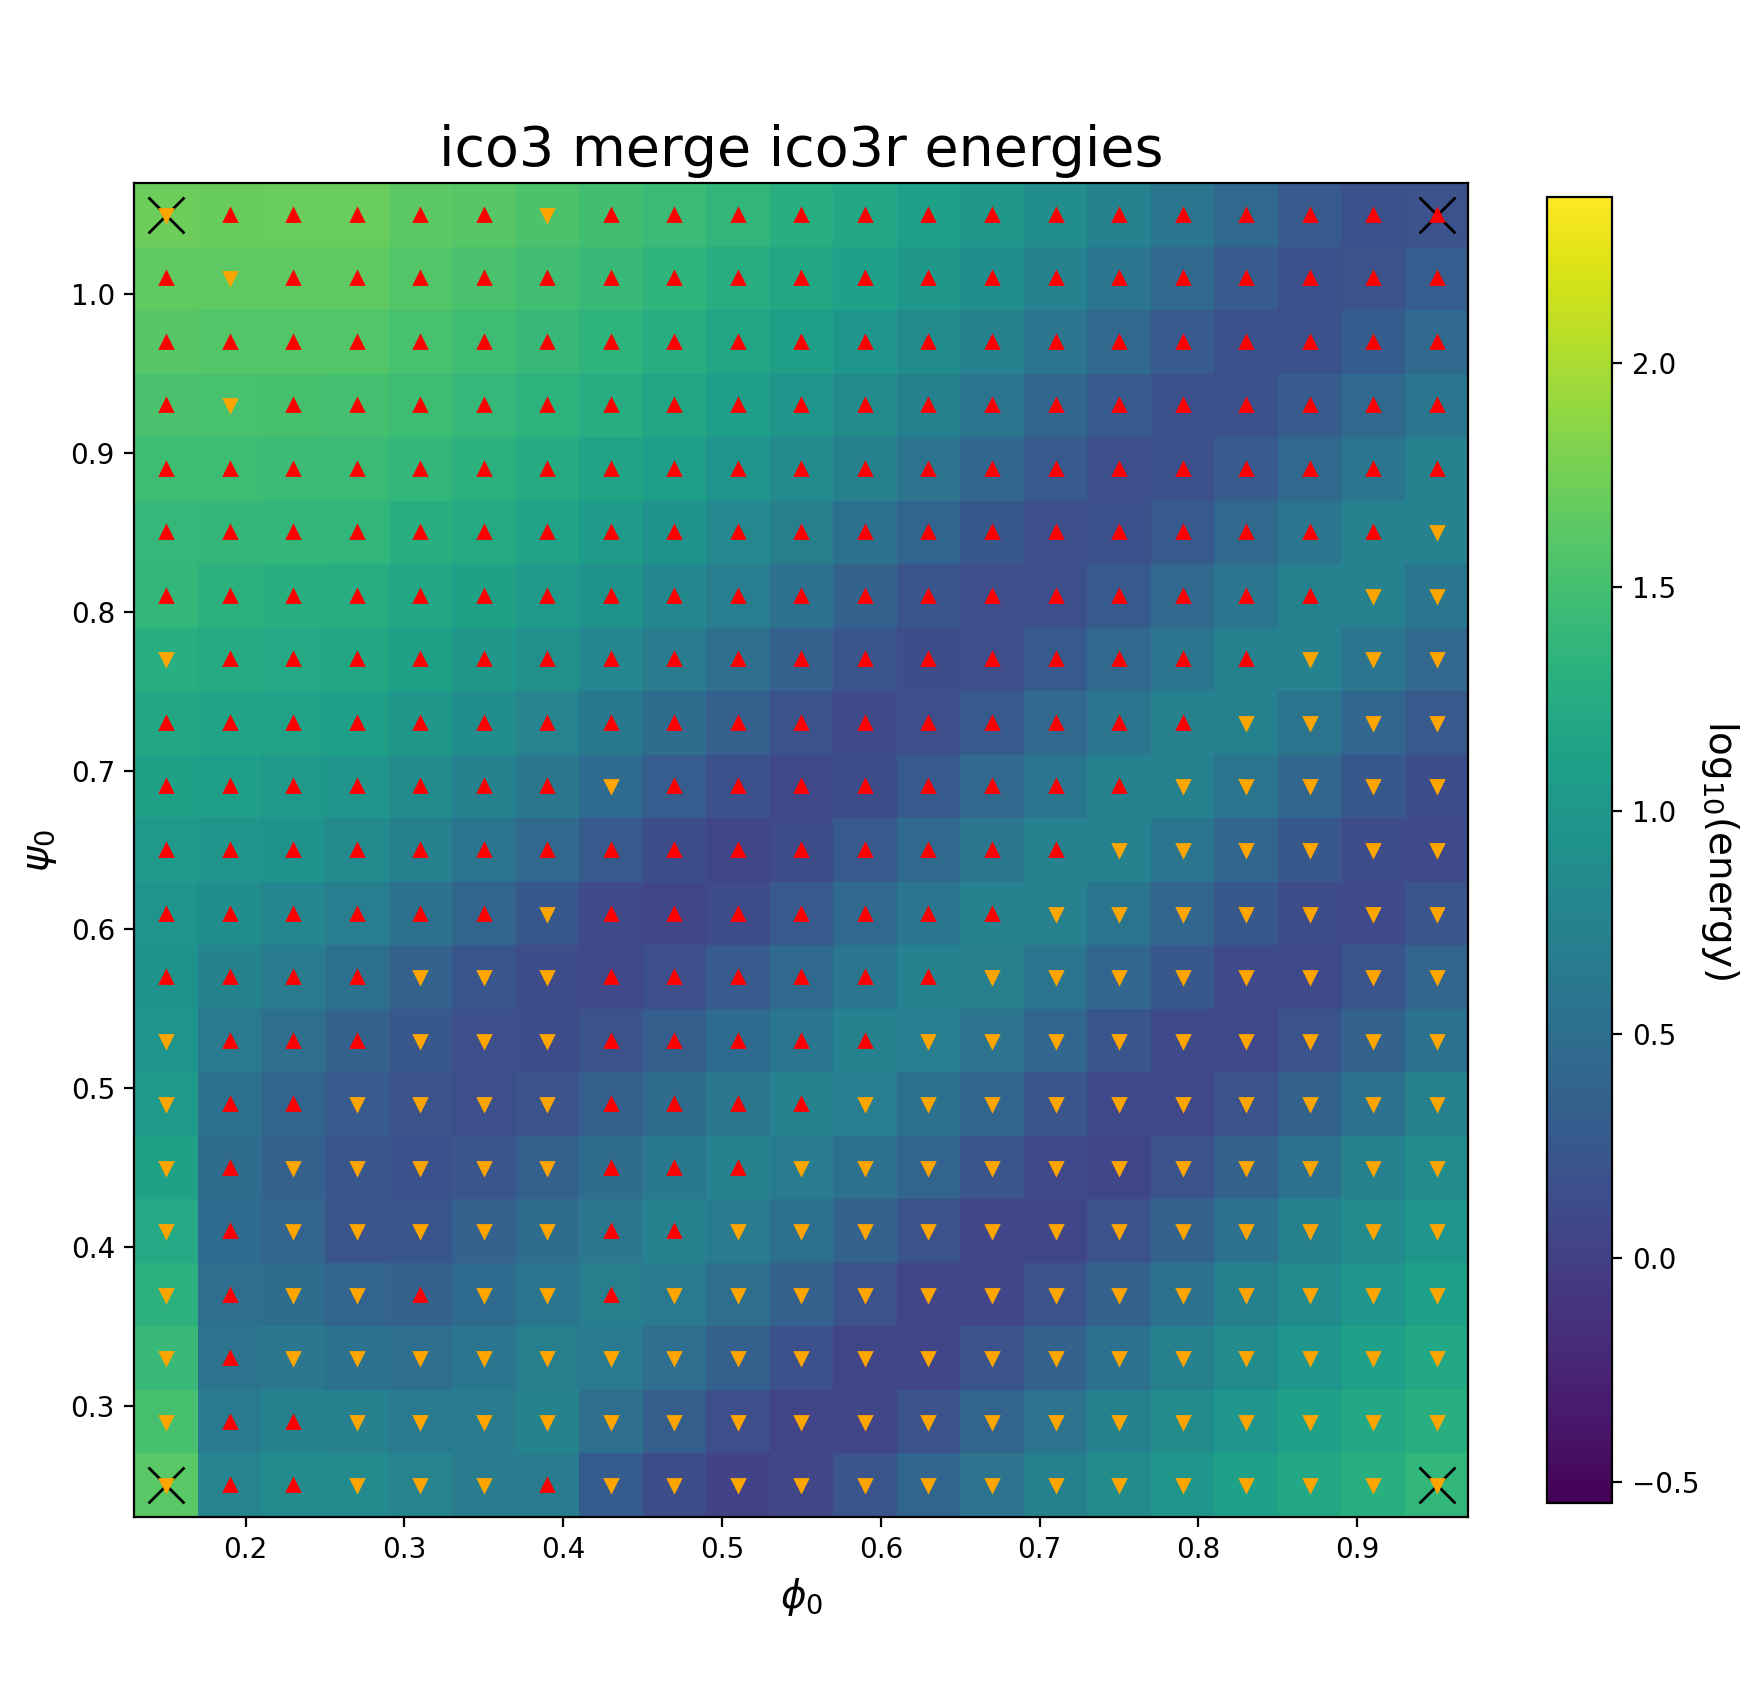
\includegraphics[width=\textwidth]{landscape_merge.png}
	\caption[Combined energy landscape of \cref{fig:landscape_ico3}]{Minimum energies the two landscapes shown in \cref{fig:landscape_ico3}. Values pulled from \cref{subfig:landscape_ico3} are denoted with red triangles and \cref{subfig:landscape_ico3r} with orange triangles.}
	\label{fig:landscape_merge}
\end{figure}

\Cref{eq:h0} describing the preferred mean curvature in terms of equilibrium constants $\phi_0$, $\psi_0$, and $\ell_0$ could be decomposed into a bending term $\sin(\psi_0 - \phi_0)$ and a length scale $\ell_0 \sin \phi_0$. 
Given the nearly constant behavior in \cref{fig:landscape_merge} along $\phi_0 = \psi_0$, it appears natural to project all points onto the orthogonal axis and plot the energy as a function of $\sin(\psi_0 - \phi_0)$. 
\Cref{fig:collapse} shows the result of plotting \cref{fig:landscape_merge} and the energies from \cref{fig:landscape_ico3} together. 
In this picture, we may interpret $\psi_0 - \phi_0$ as a state parameter to be varied causing a transition between flagella-in and -out states when sufficiently changed.

\begin{figure}[bthp]
	\centering
	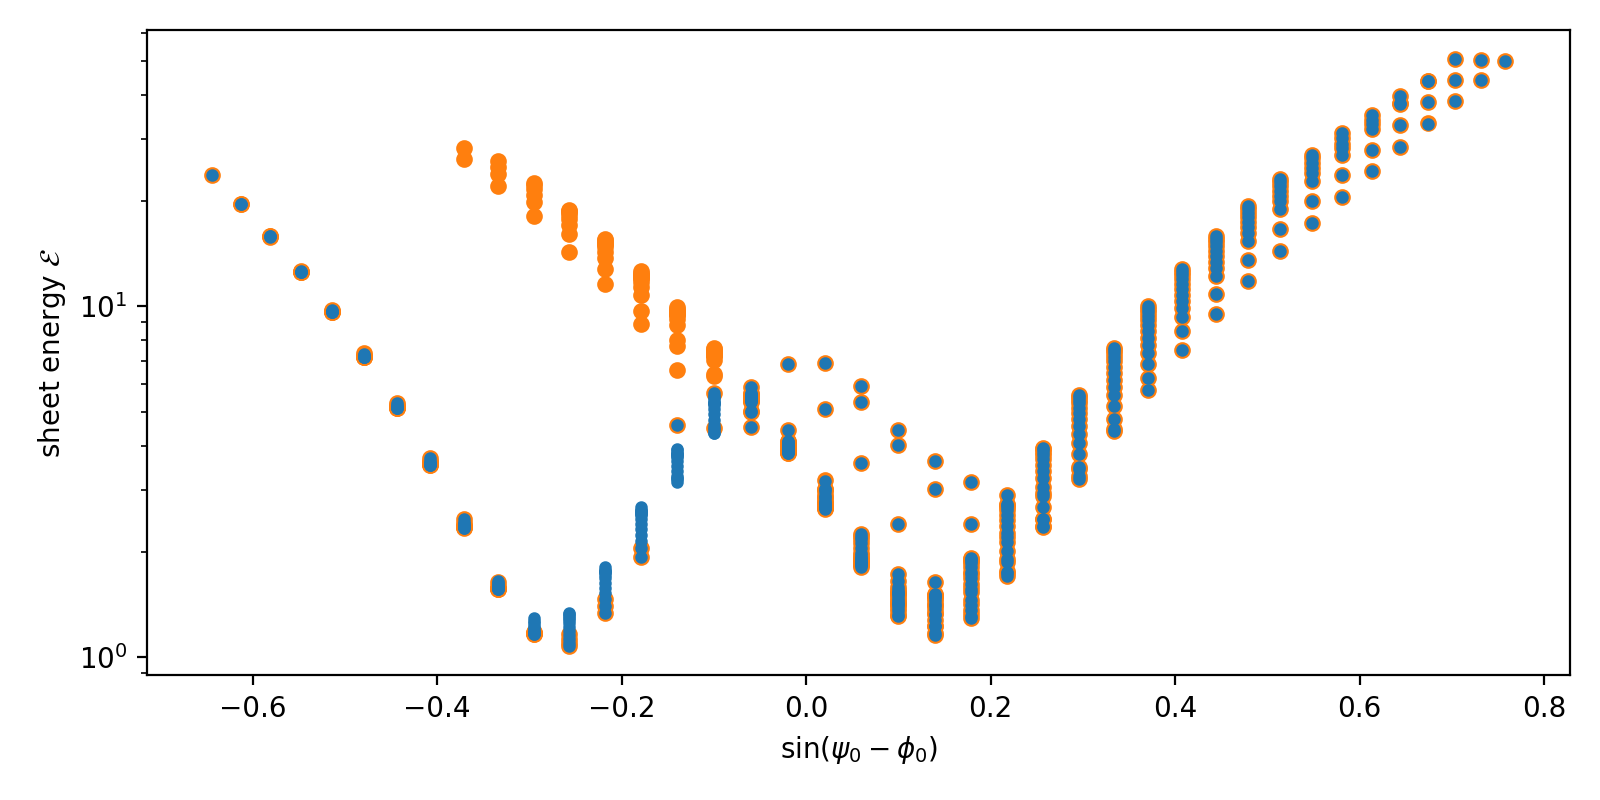
\includegraphics[width=\textwidth]{collapse.png}
	\caption[Energy landscape of an inverting sheet projected onto a single axis]{The energy landscapes in \cref{fig:landscape_merge} (blue points) and \cref{subfig:landscape_ico3} (orange, larger points) plotted as a function of $\sin (\psi_0 - \phi_0)$. Sheets beginning as flagella-in are able to exist in a stable local minimum that is not global.}
	\label{fig:collapse}
\end{figure}

\subsection{Inversion dynamics} \label{subsec:dynamics}

Informed by the transitions shown in the \cref{fig:landscape_ico3} landscape, we ask what the inversion dynamics look like in this model.
\Cref{fig:dynamics} shows the inversion from flagella-in to flagella-out by a single, sudden change in parameters.
Unlike the filament model studied in \cref{sec:c_1d} (\cref{fig:shapes}) and the small sheet in \cref{subsec:landscape}, large sheet inversion in the discrete model features temporary flattening through stretching at the edges.
The propagation of the change in curvature from the sheet boundary to the centre results in the \textit{rolling over} effect described in \cref{sec:c_1d} that is missing from those less detailed and smaller sheet descriptions. 
Notably, this is achieved with simple linear isotropic drag, supporting the hypothesis posed in \cref{sec:c_1d} that collar compression and stretching contribute meaningfully to inversion dynamics.

The continuities in \cref{fig:landscape_ico3} and inversion dynamics indicate that the topology of the cell-cell connection graph is key to producing bistability, where both flagella-in and flagella-out states are achievable as local energy minima for the same model parameters.
In contrast, a sheet without topological defects (\cref{fig:landscape_flat}) or a small sheet with fewer cells at the boundary (\cref{fig:landscape_ico}) readily inverts between states with similar energies.

Taking this further, we expect that some sheet topologies may be so restrictive at the boundary or elsewhere that inversion is completely prohibited for sufficiently high $k_{\text{sp}}$. 
Taking most of an icosphere to generate the sheet topology results in a complete inability to invert for the same energy constants used in \cref{fig:landscape_flat,fig:landscape_ico,fig:landscape_ico3}.
Instead, sheets retain their orientation always and experience substantial stress when the equilibrium angles prescribe a curvature that cannot be achieved in the present sheet orientation (\cref{fig:landscape_ico4}).
The flagella-out landscape is qualitatively similar with a valley in the same location as \cref{subfig:landscape_ico3r}.
The combined landscape of flagella-in and -out sheets (\cref{subfig:landscape4_merge}) again shows the two valleys, now separated by an insurmountable energetic barrier.

\begin{figure}
	\centering
	\begin{subfigure}[b]{\textwidth}
		\centering
		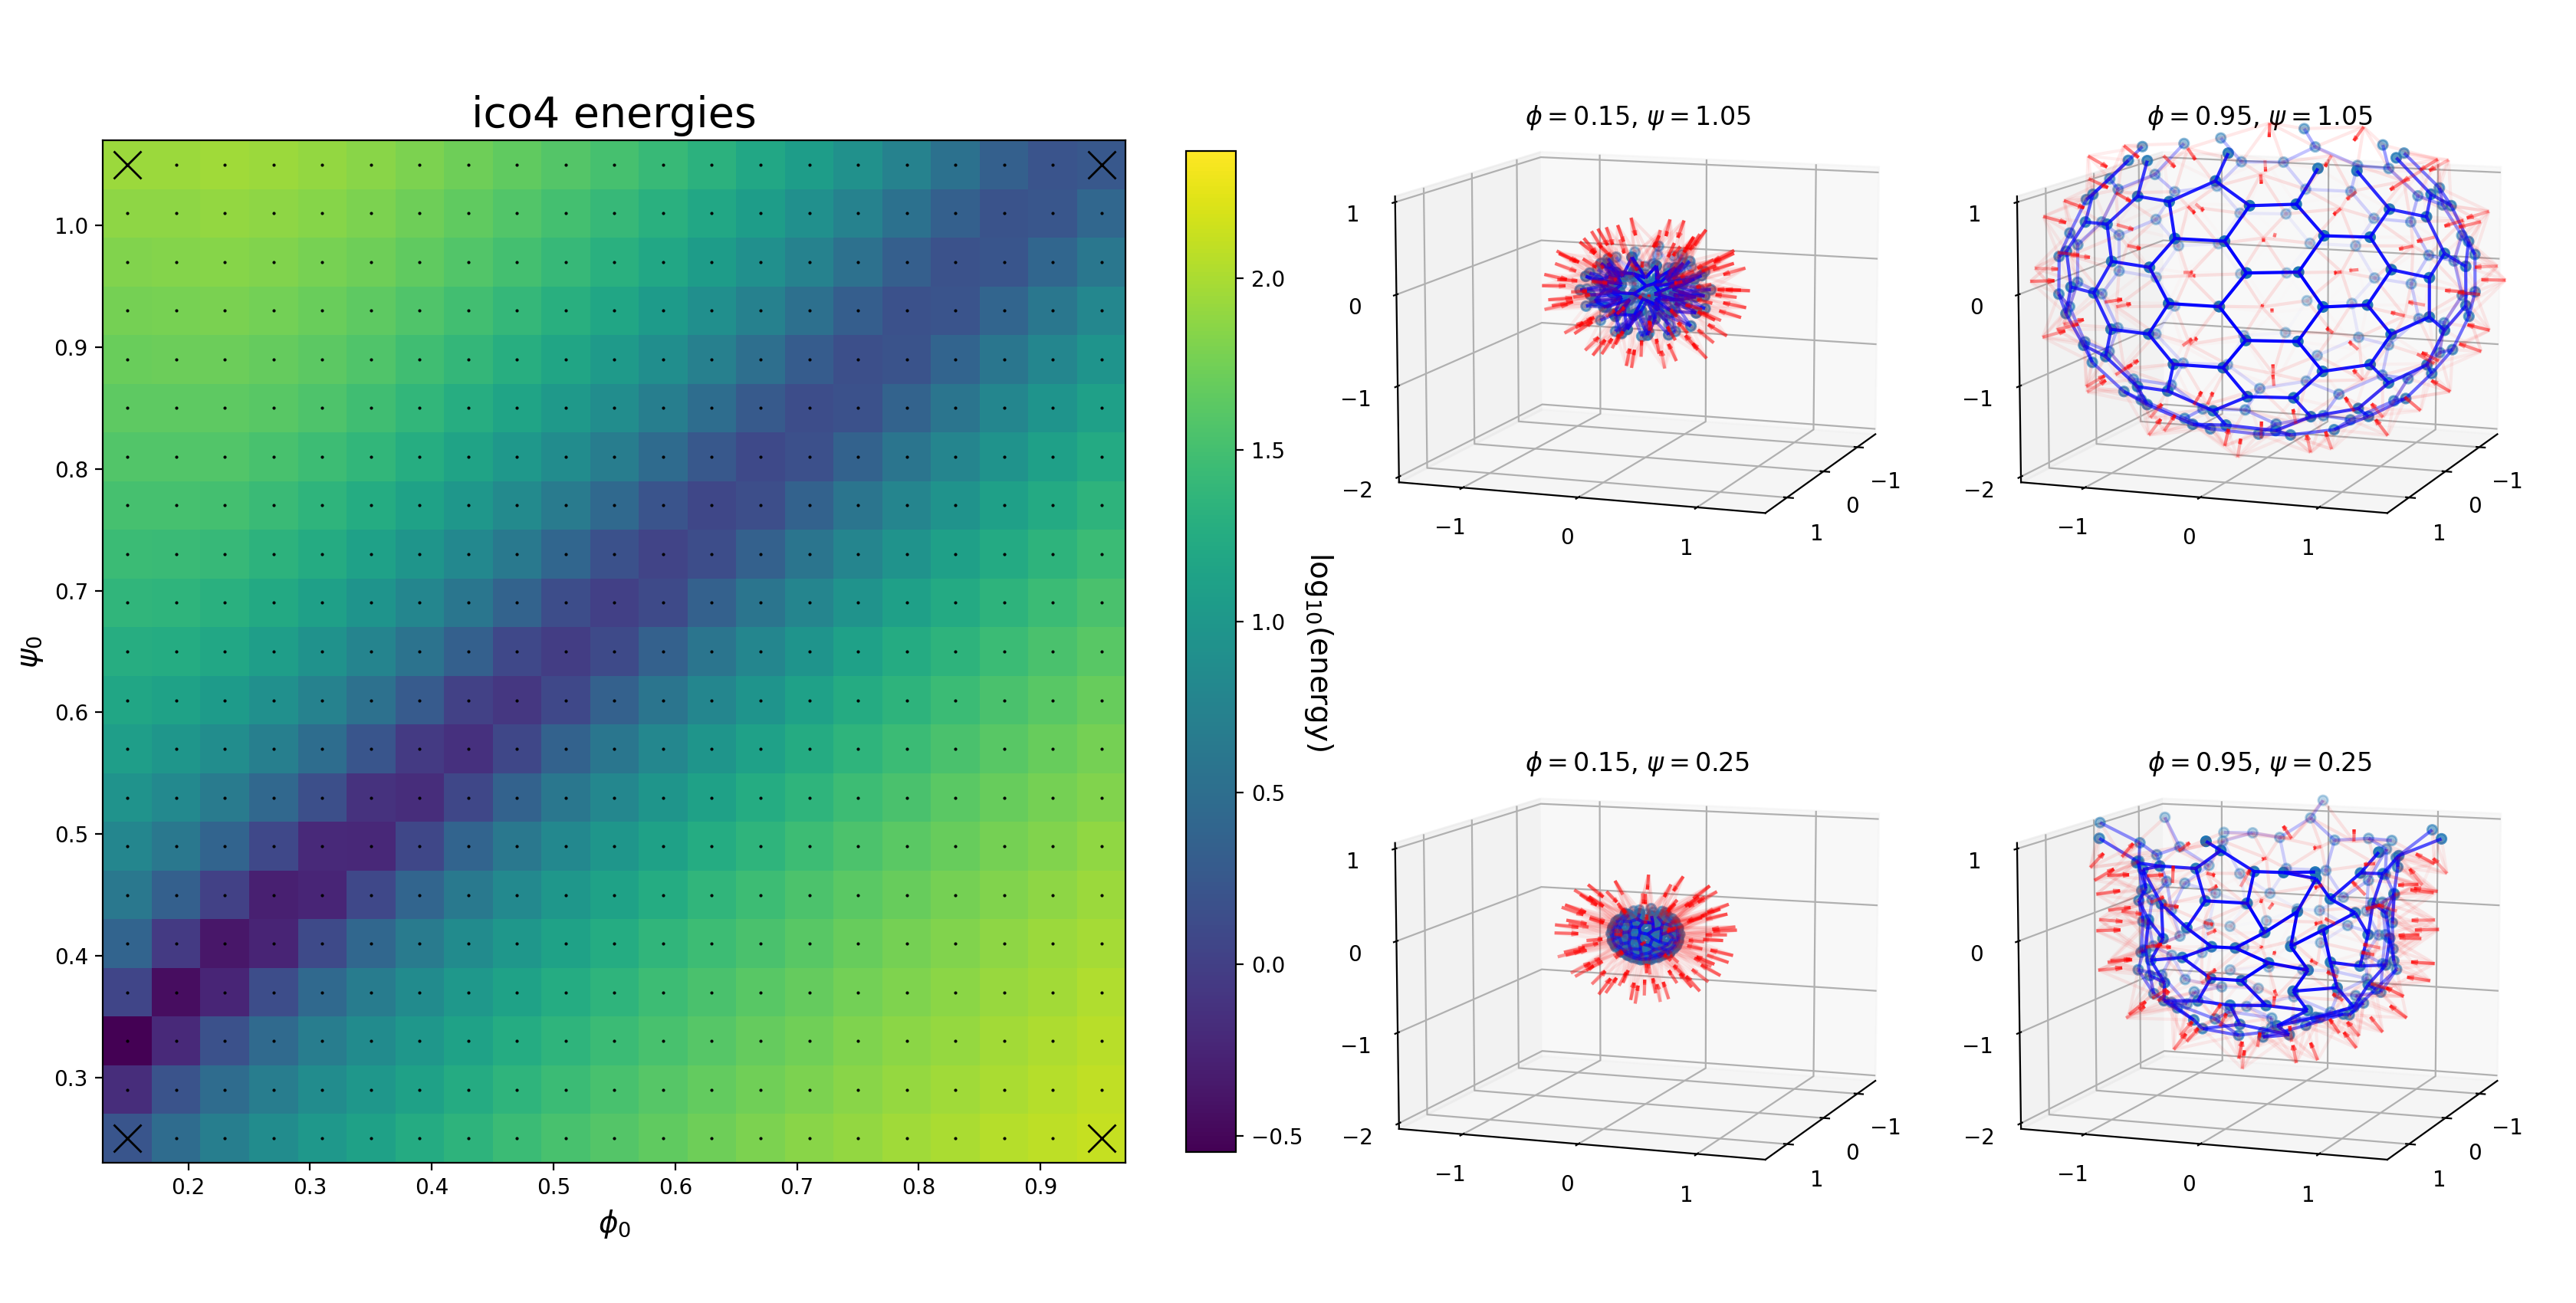
\includegraphics[width=\textwidth]{landscape_ico4.png}
		\caption{}
		\label{subfig:landscape_ico4}
	\end{subfigure}
	\begin{subfigure}[b]{\textwidth}
		\centering
		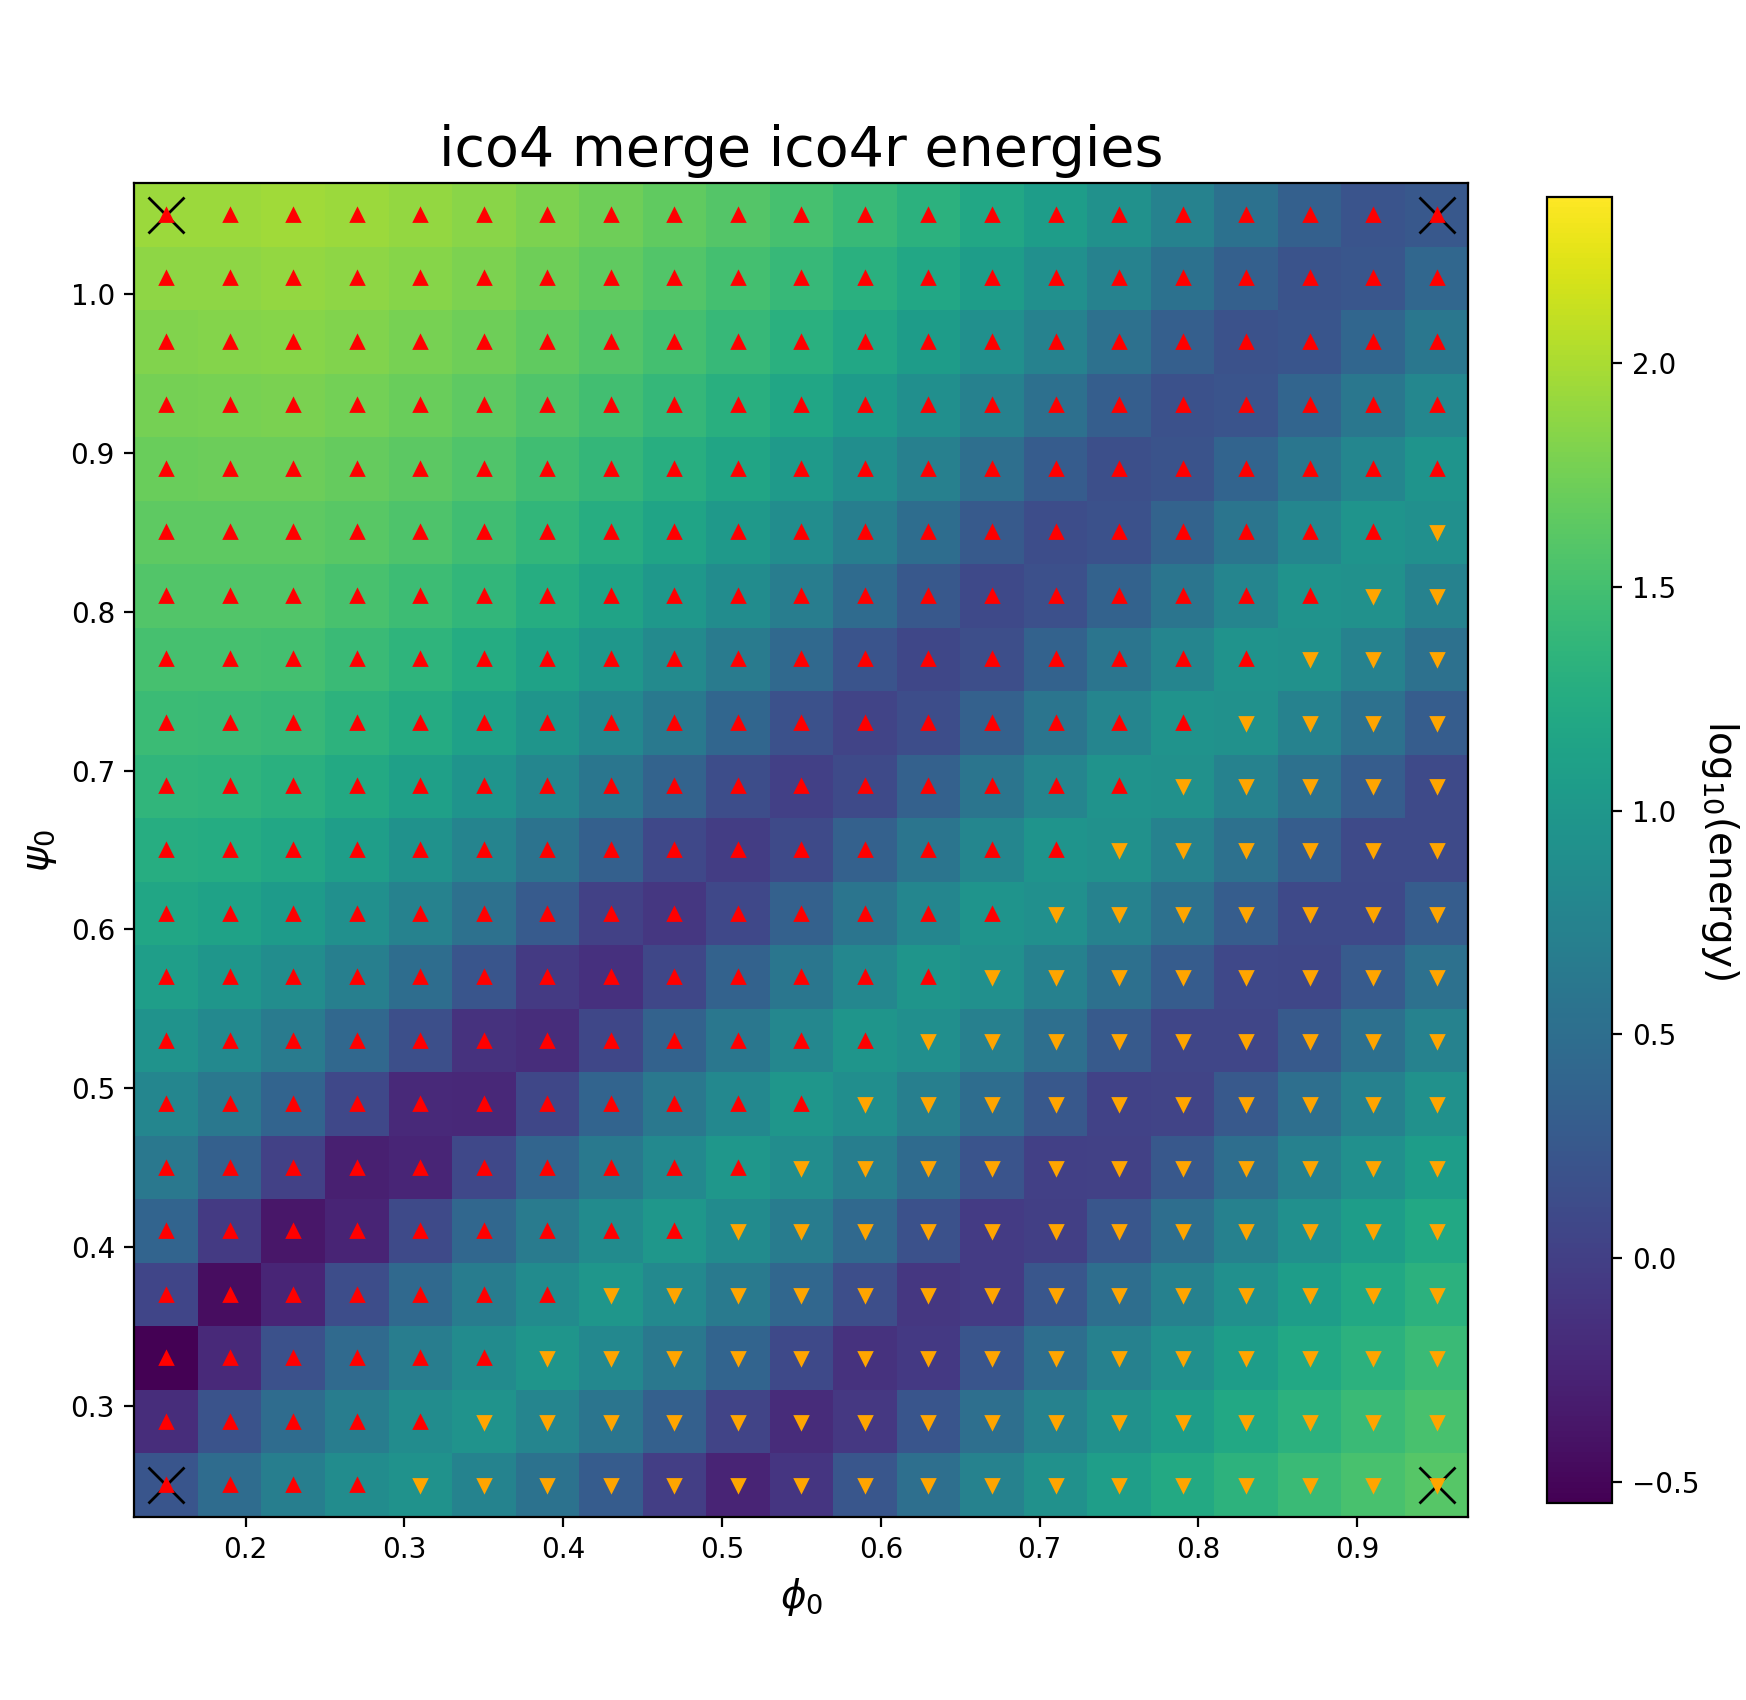
\includegraphics[width=0.8\textwidth]{landscape_ico4ico4r_merge.png}
		\caption{}
		\label{subfig:landscape4_merge}
	\end{subfigure}
	\caption[Energy landscape for flagella-in and flagella-out curved sheets]{(\ref{subfig:landscape_ico4}) Energy landscape for large flagella-in sheets. The landscape for flagella-out sheets was quantitatively similar, with the minimum energy valley shifted downward as in \cref{subfig:landscape_ico3r}. Several cells with an irregular number of neighbours are readily visible in the foreground of the top-left-most panel. (\ref{subfig:landscape4_merge}) Minimum energies for flagella-in and -out large sheets. Style as in \cref{fig:landscape_merge}.}
	\label{fig:landscape_ico4}
\end{figure}

It is clear that there may be a substantial energetic barrier to invert induced by collar-collar adhesion forces and collar stiffness. 
While this energetic barrier can be overcome by further pushing the equilibrium angles into a region that favors the opposite curvature (\cref{fig:landscape_ico3}) in simulations, \textit{C. flexa} cells appear to act in exclusively one of two pre-determined states.
There is no evidence to suggest changing collar properties, so we are led to predict that changing cell sheet topology is the factor which enables inversion.

\subsection{Additional graph topologies}

In addition to the hexagonal lattice and icosphere sections shown above, I observed that the lattice topology of the \textit{Choanoeca} sheet may restrict or force sheet bending altogether (\cref{fig:extra}).
A hexagonal lattice consisting of too many points is limited in its flexibility except at its edges (\cref{subfig:hexbig}). 
Consequently, we see that topological defects are not necessarily the hinderance to sheet bending or inversion, but rather necessary in moderation.
On the other hand, a sheet with many topological defects with topology formed by generalised Voronoi tesselation on the sphere using several random points is extremely restricted in curvature when there are too many points crowding a small region (\cref{subfig:sphere}).

\begin{figure}[bhtp]
	\centering
	\begin{subfigure}[b]{0.48\textwidth}
		\centering
		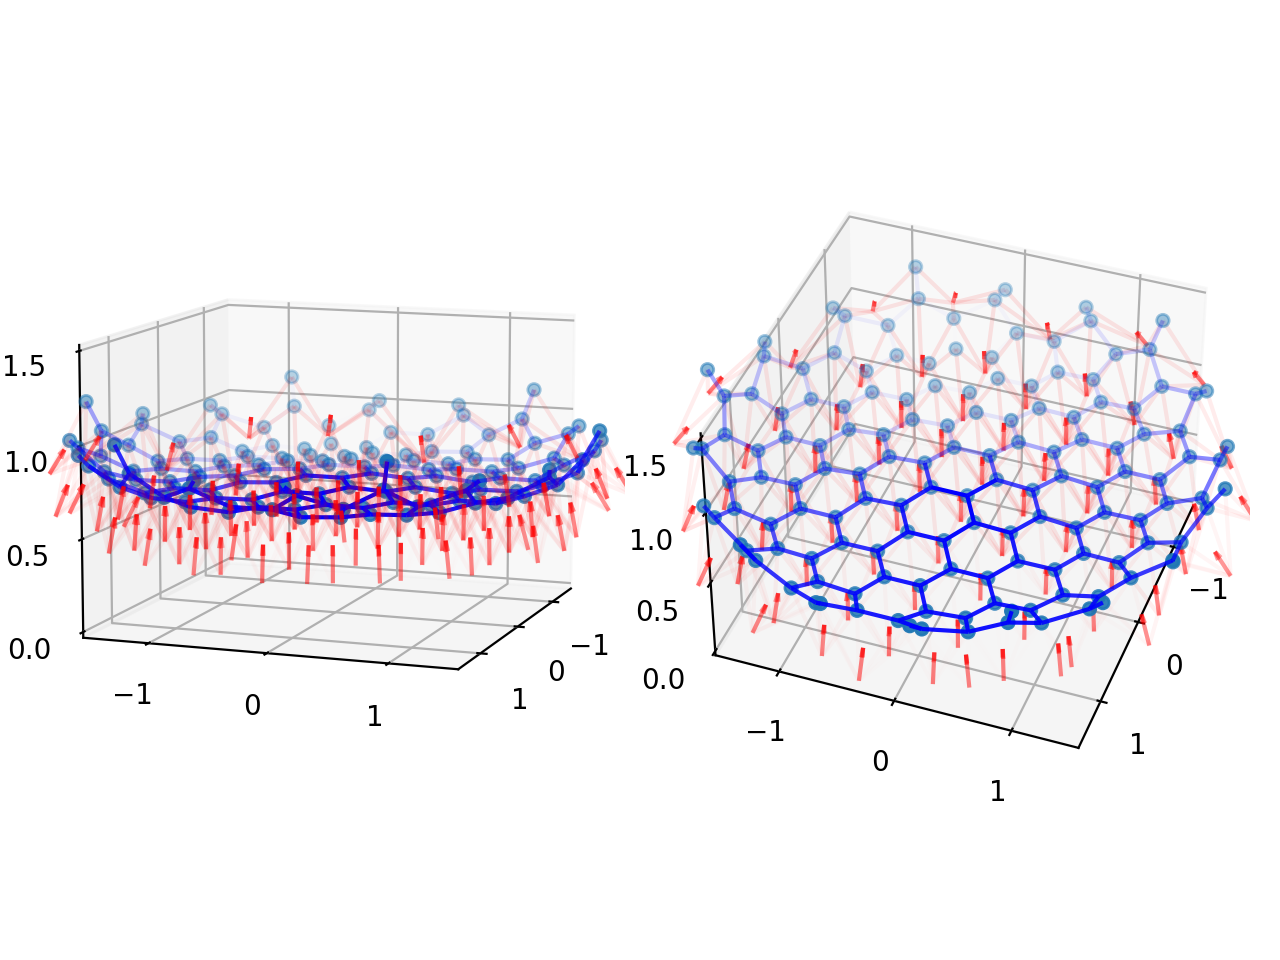
\includegraphics[width=\textwidth]{hexbig.png}
		\caption{}
		\label{subfig:hexbig}
	\end{subfigure}
	\begin{subfigure}[b]{0.48\textwidth}
		\centering
		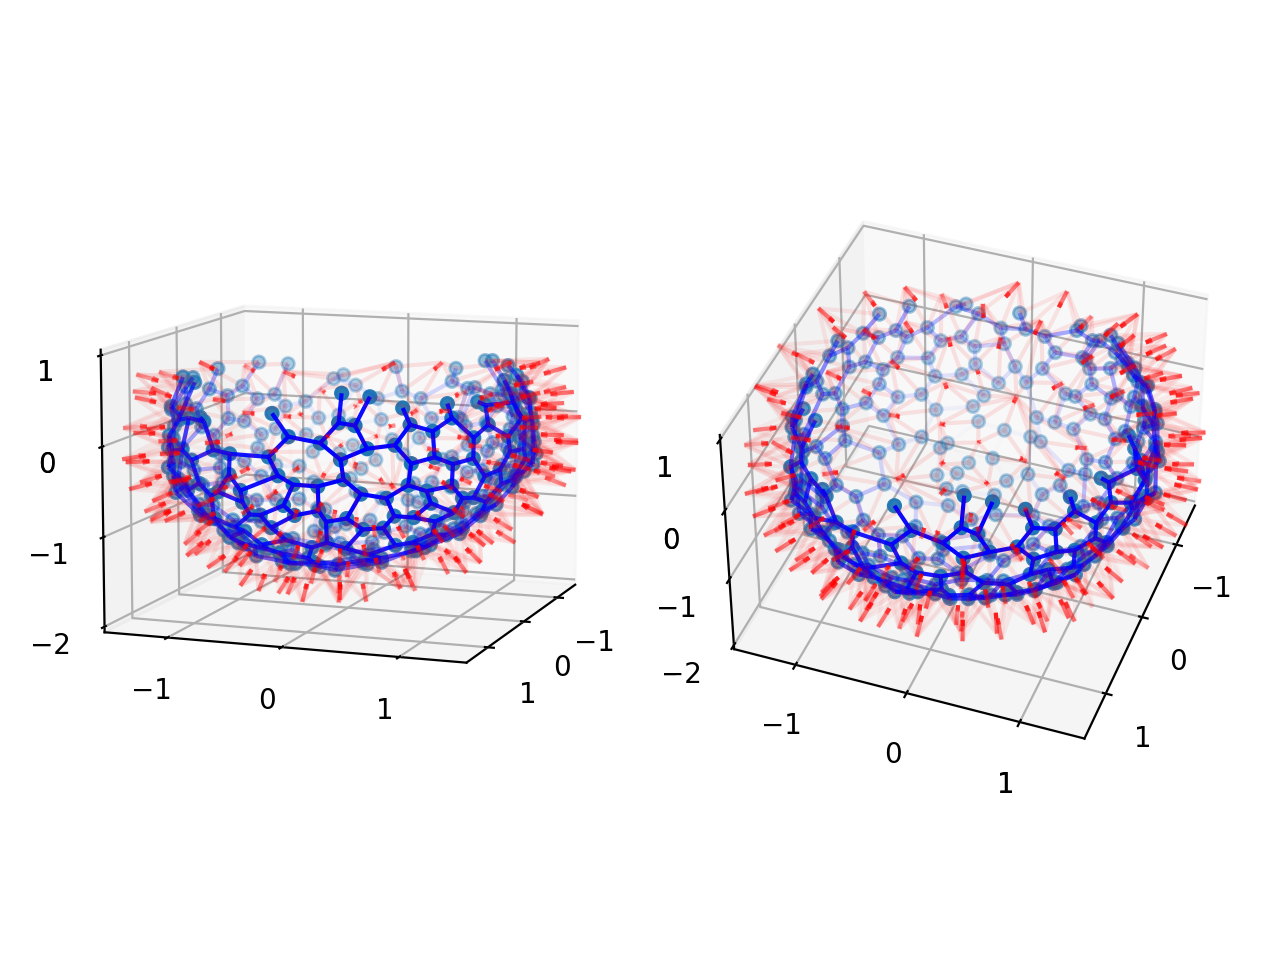
\includegraphics[width=\textwidth]{sphere.png}
		\caption{}
		\label{subfig:sphere}
	\end{subfigure}
	\caption[Equilibrium sheets of other lattice topologies]{Equilibrium sheets of additional lattice topologies. (\ref{subfig:hexbig}) Two views of a large hexagonal lattice sheet with $\phi_0 = 0.6$, $\psi_0 = 0.8$. Note that this angle caused substantial bending in \cref{fig:landscape_flat}. (\ref{subfig:sphere}) Two views of a sheet defined by Voronoi tesselation on random points on a sphere. The sheet was almost entirely rigid regardless of angles $\phi_0, \psi_0$ used.}
	\label{fig:extra}
\end{figure}

\mynote{Discuss that the phi and psi energies are around an order of magnitude higher than the spring energy? awaiting results from relaxing $k_{\text{sp}}$. Maybe it's really that you can't get expansion in collars at the boundary without expansion at the center too}

\begin{comment}
\begin{align*}
    \vec{F}_\gamma = \frac{\partial E}{\partial \vec{r}_\gamma} &= 2 \sum_{(\alpha, \rho)} \left( \phi_{(\alpha,\rho)} - \phi_0 \right) \frac{\partial \phi_{(\alpha,\rho)}}{\partial \vec{r}_\gamma} + 2 \sum_{(\alpha, \beta: \sigma, \rho)} \left( \psi(\hat{\bm{n}}_{\sigma\alpha\rho}, \hat{\bm{n}}_{\sigma\beta\rho}) - \psi_0 \right) \frac{\partial \psi_{(\alpha, \beta: \sigma, \rho)}}{\partial \vec{r}_\gamma} \\
    \frac{\partial \phi_{(\alpha,\rho)}}{\partial r_{\gamma i}} &= \frac{-1}{\sqrt{1 - (\hat{\bm{n}}_\alpha \cdot \hat{(\alpha\rho)})^2}} \left(\frac{\partial \hat{\bm{n}}_{\alpha j}}{\partial r_{\gamma i}} \hat{(\alpha\rho)}_j + \frac{\partial \hat{(\alpha\rho)}_j}{\partial r_{\gamma i}} \hat{\bm{n}}_{\alpha j} \right) \\
    \frac{\partial \hat{(\alpha\rho)}_j}{\partial r_{\gamma i}} &= \frac{(\delta_{\gamma\rho} - \delta_{\gamma\alpha})}{|r_\rho - r_\alpha|} \left( \delta_{ij} + \hat{(\alpha\rho)}_i\hat{(\alpha\rho)}_j \right) \\
    \frac{\partial \hat{\bm{n}}_{\alpha j}}{\partial r_{\gamma i}} &= \frac{\mathbb{1}_{\gamma\in \text{collars}(\alpha)} - n\delta_{\gamma\alpha}}{\left| \sum_{(\alpha, \rho)} (r_\rho - r_\alpha) \right|} \left(\delta_{ij} - \hat{\bm{n}}_{\alpha i} \hat{\bm{n}}_{\alpha j} \right) \\
    \frac{\partial \psi_{(\alpha, \beta: \sigma, \rho)}}{\partial r_{\gamma i}} &= \frac{-1}{\sqrt{1 - (\hat{\bm{n}}_{\rho\alpha\sigma} \cdot \hat{\bm{n}}_{\rho\beta\sigma}})^2} \left(\frac{\partial \hat{\bm{n}}_{\rho\alpha\sigma j}}{\partial r_{\gamma i}} \hat{\bm{n}}_{\rho\beta\sigma j} + \frac{\partial \hat{\bm{n}}_{\rho\beta\sigma j}}{\partial r_{\gamma i}} \hat{\bm{n}}_{\rho\alpha\sigma j} \right) \\
    \frac{\partial \hat{\bm{n}}_{\rho\alpha\sigma j}}{\partial r_{\gamma i}} &= \text{too big see notes}
\end{align*}
\end{comment}

%!TEX root = ../thesis.tex
%*******************************************************************************
%*********************************** Fourth Chapter ****************************
%*******************************************************************************

\chapter{Discussion} %Title of the First Chapter

\ifpdf
    \graphicspath{{Chapter4/Figs/Raster/}{Chapter4/Figs/PDF/}{Chapter4/Figs/}}
\else
    \graphicspath{{Chapter4/Figs/Vector/}{Chapter4/Figs/}}
\fi

The modeling done here offers several perspectives to study the mechanics of sheet shape and inversion in \textit{Choanoeca}. 
We see that the discrete, lattice structure of the sheet makes the sheet's intrinsic curvature possible, and the sheet's curvature emerges in response to the lattice structure.
The presence of topological defects gives a tight ring of cells at the sheet boundary, which presents an energetic challenge during inversion.
The models that I built make it clear that stretching plays a major role in the dynamics of sheet inversion, and they distill the essential mechanics of \textit{C. flexa} colony shape to only two parameters.
This discrete model of sheet inversion supports the hypothesis that \textit{C. flexa} inverts using an instantaneous active change of collar microvillus preferred shape.

%********************************** %First Section  **************************************
\section{\textit{C. flexa} geometry} 

% what does this work achieve
\textit{Choanoeca} differs from its relatives in that it lacks an extracellular matrix, which is responsible for producing disks, cups, or branched trees with flagella splayed out in other species' colonies \citep{larson2020}. 
Despite lacking an ECM, these colonies are able to achieve large-scale geometric changes that are believed to faciliate function \citep{brunet2019}.
In this work, I show that a simple model which distills collar filament mechanics into a few descriptive angles $\phi, \psi$ and filament lengths is sufficient to capture the curvature of whole sheets and their inversions following a rapid stimulus, here captured by an instantaneous change in preferred angles $\phi_0$ and $\psi_0$.
While we can develop increasingly complex models by introducing collar filament bending, tension and stress at the collar filaments' bases, or the effects of the contractile ring, I demonstrate here that a coarse description of individual cells is sufficient to explain the behavior that we observe in colonies. 
Compare this with \textit{Volvox}, which uses connections and communication between cells to control its inversion. 
One might imagine that the complexity of a molecular pathway for a single cell to exhibit phototaxis or regulate feeding/swimming efficiency could easily exceed that of the ring contraction as currently understood in \textit{C. flexa} \citep{brunet2019}. 
\mynote{cite Volvox inversion papers, cite papers on phototaxis or swimming signalling pathways}

% why have a curved sheet?
While the modelling in this work captures the mechanics underlying sheet curvature, it does not identify environmental pressures that may have selected for the morphology exhibited by \textit{Choanoeca} colonies.
The small curvature in \textit{C. flexa} colonies permit them to drive strong flows by aligning their apicobasal axes close to parallel while simultaneously producing two stable shape equilibria.
This contrasts with the rosette colonies of \textit{S. rosetta}, which are known to have morphology inefficient for driving feeding flows \citep{kirkegaard2016}.
\textit{C. flexa} may also be driven to form the observed monolayers of cells because this morphology allows cells more flow of their own for feeding.
Nevertheless, there may be a myriad of other reasons that these species have evolved to have their current morphologies, especially external influences from the ecosystems they inhabit.

% why does choanoeca align as it does
\textit{Choanoeca} is remarkable in the common orientation of all cells in its colonies, which is made possible by its colonies' connections via collar filaments rather than an extracellular matrix \citep{leadbeater1983}. 
It is clear that the collar filaments are essential to the sheet orientation, and that they are the means by which sheets achieve variable curvature.
My work here reduces the complexities of these filaments significantly by representing their bending energies with simple terms based on the angles they make and their end-to-end distances.
Moreover, my discrete model treats the line of filament interactions between two neighbouring cells as a line of many infinitesimal filaments.
A more complete model would explore the details of filament mechanics between cells.
Doubtless, further work on the detailed mechanics contributing to sheet geometry must be guided by experiments.
In particular, it is currently unclear how collar filaments adhere to those of other cells in a seemingly selective way (\cref{subfig:contact1,subfig:contact2}).

\section{Discrete cell sheet topology}

% what did I find about lattice topology?
The discrete model of \textit{C. flexa} demonstrates that deviations from a hexagonally packed sheet at as few as one cell are sufficient to induce substantial bending.
This result is consistent with that described in \citet{seung1988} for planar lattices, albeit through a different mechanism where stretching and bending are closely related.
Indeed, topological defects induce buckling and non-local inability to satisfy equilibrium conditions, yet these defects are also vital to achieving large-scale sheet curvature.
The model I develop in \cref{ch:3} supports the idea that, loosely, defects in the small-scale lattice topology induce curvature in the large-scale sheet geometry.
While not previously explored, we should expect to find a small but non-negligible fraction of cells in \textit{Choanoeca} colonies to have an irregular number of neighbours.
Further imaging as in \cref{subfig:contact1},\ref{subfig:contact2} to quantify the statistics of the numbers of neighbours in colonies would be valuable.

% what do we actually observe and how does it line up with the model used here?
\citet{leadbeater1983} describes that in \textit{C. perplexa} colonies, each cell is typically adjacent to six others. 
Given the strong \textit{Choanoeca} sheet curvatures and known association between Gaussian curvature and topological defects in lattice structure (\cref{subsec:cts}) \citep{sachdev1984,seung1988}, it is reasonable to expect that many cells have more or fewer than six neighbors.
Even in a small section of the colony \cref{subfig:contact1}, several defects may be readily identified.

% How reasonable was this model?
Physical reasoning suggests that interfaces between cells would be equidistant from the cell bodies, since each cell is assumed to be identical and the forces must balance at equilibrium. 
Imaging supports this idea (\cref{fig:cflexa}), though any imaging requiring fixation may affect the collar stiffness or preferred curvature.
That the collar microvilli at the boundaries form an arc around the apicobasal axis suggests that they freely take angle $\phi_0$ at the base and do not contribute meaningfully to the energy (\cref{subfig:contact2}). 
This validates the treatment of boundary collar vertices used in the discrete model.

\section{Extensions}

% studying what prevents inversion
Both the continuous and discrete models developed make clear that azimuthal stretching in curved sheets is critical in \textit{C. flexa} inversion, especially by introducing an energetic barrier.
With even relatively large-area sheets observed inverting readily in culture (collar diameter relative to sheet major-axis diameter as low as $\sim20\%$), collar-collar interfaces must either be able to substantially stretch or connections must break.

% more detailed flow
The simple, continuous one-dimensional model of \cref{sec:c_1d} had two clear limitations discussed there: the lack of chain elongation or shortening and the assumption of linear, isotropic drag.
The results discussed in this work support the hypothesis that the former is largely responsible for \textit{Choanoeca} colony shape.
However, the extent to which flow affects sheet shape is unclear, both in experimental results \citep{brunet2019} as well as the larger theoretical work this thesis contributes to.
Linear, local isotropic drag would suggest a chain of cells falling through the fluid has the same shape as it falls, yet intuitively we expect the ends of the chain to lag behind its centre.
I expect that the effect would be less pronounced in a two-dimensional sheet since azimuthal stretching and compression generally appear to restrict sheet shape (\cref{fig:extra}), though there are nevertheless many questions to explore relating flow and geometry.
Consequently, we should be careful to draw conclusions from details in the dynamics of the models presented here, including \cref{fig:shapes} and \cref{fig:dynamics}.
Since the shape changes in the discrete model are slow relative to the timescale defined by system size and fluid properties, it is compelling to at least treat sheet boundaries rolling over as a consequence of topological constraints.
Our understanding of flow's impact on colony shape would be improved greatly by experiments placing colonies near surfaces or in external flows and observing any changes in shape.

% describing colony growth and resulting lattice topology
A model for \textit{Choanoeca} colony growth may help understand the origins and distributions of topological defects in the lattice structure. 
Given the possible division strategy of these cells (\cref{fig:division}) and the idea that other choanoflagellate colony cells divide without synchronisation \citep{larson2020}, we might build a model by spontaneously splitting cells into pairs of adjacent daughter cells.
The goal of a colony growth model is two-fold.
First, a model for colony growth may explain the origin of topological defects in \textit{C. flexa} colonies.
We would obtain graph topological statistics that are comparable to experiments to determine if this method of colony growth is accurate or if another method produces the observed topological defects.
Second, such a model may cause the cup-like sheets observed, rather than sheets with other complex geometries.
Moreover, the distribution of defects over the sheet may produce non-icosahedral or -spherical equilibrium geometries, as large \textit{Choanoeca} sheets tend to be ellipsoidal rather than spherical \citep{leadbeater1983,brunet2019}.
It remains to be resolved how colonies form without buckling at sheet boundary: uniform, isotropic cell division would give proportionally scaling area and boundary length, but preferred sheet curvature would cause buckling with too large of a boundary.
We can consider this as a conflict between preferred sheet curvature with bending based on $\sin (\psi_0 - \phi_0)$ and preferred cell space based on $\ell_0 \sin \phi_0$ (\cref{eq:h0}).
Experimental observations of colonies as they grow and divide would validate a model for growth, as well as provide some insight into the formation, coordination, and persistence of collar-collar connections.

% alternative colony growth theorising
An alternative theory for \textit{Choanoeca} colony growth is via aggregation \citep{grosberg2007}, though choanoflagellate colonies have only been observed to form by clonal division \citep{fairclough2010,alegado2012,woznica2016}.
Sequential cell adhesion at the boundary would resolve buckling at the edges due to uniform, isotropic growth.
Moreover, aggregation resolves the issue that there are a discrete number of microvilli at cell-cell interfaces.
Hence, the interfaces cannot be divided between daughter cells indefinitely.
Recent evidence from \textit{S. rosetta} points that several processes involved in maintaining the colony ECM are involved in preventing spurious aggregation \citep{wetzel2018}, indicating that aggregation is specifically disfavored in other choanoflagellates.
Colony formation by aggregation is unprecendented in our understanding of choanoflagellates, and of course comes with the organisational challenge of producing a single consistent orientation over the entire sheet.

% changing lattice topology to induce inversion
While the structures used in this work had discrete symmetry around an axis, \textit{C. flexa} sheets observed experimentally may have substantial irregularities both in the bulk and at the boundary. 
Several images in \citet{brunet2019} show uneven sheet boundaries, resembling crenellations of a castle wall (\cref{fig:edges}).
As suggested in \cref{subsec:dynamics}, a sheet with excessively restrictive lattice topology may be able to achieve inversion by a temporary change in its cell-cell connections, especially by tearing or forming holes in the sheet.
Continued experimental work should look for disconnections between adjacent cells between inversion.
An extreme example of inversion through topological change is performed by \textit{Volvox} embryos, which invert by creating a hole in their sphere and pass the entire sheet through the hole \citep{hohn2015}.
Type-A \textit{Volvox} inversion forms this hole by making four lips and peels them back to begin inversion at the boundary, similar to how inversion proceeds in \cref{fig:dynamics} \citep{viamontes1977}.
Even besides boundary ruggedness, asymmetry in the sheet may promote the initiation of inversion at one region of the boundary while it is not yet possible elsewhere.

% how do colonies break apart?
\citet{leadbeater1983} described that large \textit{C. perplexa} sheets may take irregular shapes such as ribbons. 
Either as a consequence of tearing during inversion or itself causing tearing during inversion, such unusual geometries may be involved in colony division.
If colonies tear, we would not expect them to fully separate since a single connection at the boundary of either colony fragment would not hinder inversion. 
Consequently, it is possible that the weight of colony fragments themselves in the flagella-in state (with resulting incompatible drag tensors) or the strong collective flows driven by separate colony fragments in the flagella-out state are responsible for separating colony fragments.
If entirely physically facilitated, colony division is likely to substantially involve both cell-cell connection lattice structure and flows.

% assuming all cells are the same
An underlying assumption throughout this work is that \textit{Choanoeca} colonies consist entirely of identical cells, both in genetics and morphology.
Recent findings in \textit{S. rosetta} suggest that choanoflagellates are capable of spatial differentiation within colonies \citep{laundon2019,naumann2019}.
Different properties throughout the cell-cell connection network, especially different preferred collar shapes due to cell body morphology or filament mechanics, substantially affect inversion dynamics.
Most substantial would be if some adjacent cells do not form adhesive contact at all, in contrast to our current interpretation of \textit{Choanoeca} colony imaging \citep{brunet2019}.

\begin{figure}
	\centering
	\begin{subfigure}[b]{0.46\textwidth}
		\centering
		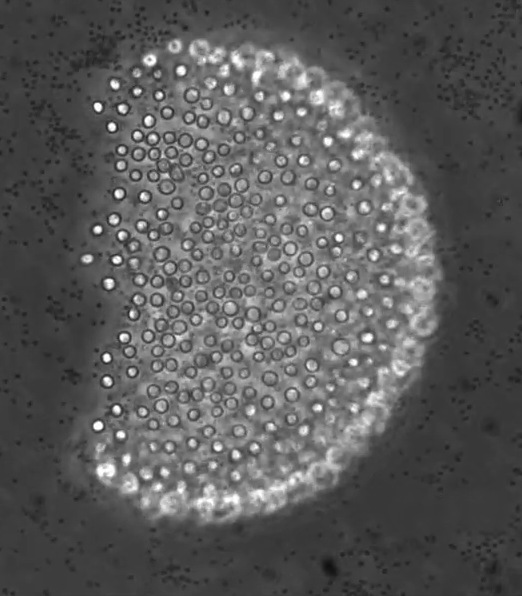
\includegraphics[height=\textwidth,angle=90]{edges1.png}
		\caption{}
		\label{subfig:edges1}
	\end{subfigure}
	\begin{subfigure}[b]{0.49\textwidth}
		\centering
		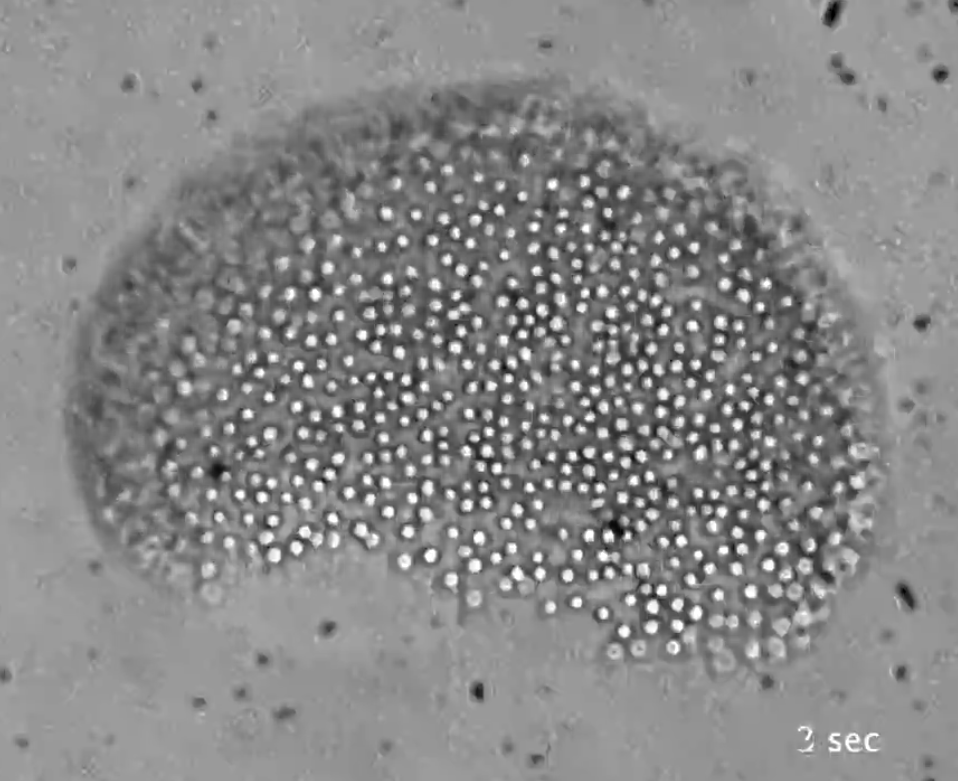
\includegraphics[width=\textwidth]{edges2.png}
		\caption{}
		\label{subfig:edges2}
	\end{subfigure}
	\caption[\textit{C. flexa} sheets with ragged boundaries]{\textit{C. flexa} sheets with ragged boundaries. From \citet{brunet2019}. Reprinted with permission from AAAS.}
	\label{fig:edges}
\end{figure}

\section{Multicellularity and \textit{C. flexa}}

% \textit{C. flexa} contrasts with volvocine algae because it does not connect cells via cytoplasmic bridges, which is a substantial difference between the two models. 
% It is not completely clear that \textit{C. flexa} sheets form with a temporary incomplete cytokinesis stage as in the algae \citep{green1981,herron2015}.

Ultimately, multicellularity in \textit{Chonoaeca} appears to be the result of a tradeoff between a decrease in the flow efficiency of individual choanoflagellate cells and the ability of the colony to invert. 
Inversion is highly dependent on the sheet structure and its lattice, which may itself change to facilitate inversion and potentially colony divison. 
A more complete experimental characterisation of \textit{Choanoeca} colonies would further inform the models developed here and clear up the connection between lattice topology, inversion, colony formation, and colony division.
Nevertheless, the multicellular mechanics of \textit{C. flexa} are crucial to its inversion and the behavior that inversion make possible.

%\include{Chapter5/chapter5}
%\include{Chapter6/chapter6}
%\include{Chapter7/chapter7}



% ********************************** Back Matter *******************************
% Backmatter should be commented out, if you are using appendices after References
%\backmatter

% ********************************** Bibliography ******************************
\begin{spacing}{0.9}

% To use the conventional natbib style referencing
% Bibliography style previews: http://nodonn.tipido.net/bibstyle.php
% Reference styles: http://sites.stat.psu.edu/~surajit/present/bib.htm

\bibliographystyle{apalike}
%\bibliographystyle{unsrt} % Use for unsorted references  
%\bibliographystyle{plainnat} % use this to have URLs listed in References
\cleardoublepage
\bibliography{References/references} % Path to your References.bib file


% If you would like to use BibLaTeX for your references, pass `custombib' as
% an option in the document class. The location of 'reference.bib' should be
% specified in the preamble.tex file in the custombib section.
% Comment out the lines related to natbib above and uncomment the following line.

%\printbibliography[heading=bibintoc, title={References}]


\end{spacing}

% ********************************** Appendices ********************************

\begin{appendices} % Using appendices environment for more functunality

%!TEX root = ../thesis.tex
% ******************************* Thesis Appendix A ****************************
\chapter{Continuous energy functional derivation} \label{apx:cts}

\Cref{ch:2} expresses an integral to evaluate the energy density at a given point in terms of constants $a, b, c, d, e$. 
\begin{align*}
    \int_{-\pi}^\pi (\phi - \phi_0)^2 d\theta &= \int_{-\pi}^\pi \frac{\left(a\cos^2\theta + b\sin^2\theta + 2c\sin\theta\cos\theta + d \right)^2}{\left(a\cos^2\theta + b\sin^2\theta + 2c\sin\theta\cos\theta + e \right)^2} d\theta \\
    &= \left\{-\sin2\theta \left[a^2 (-4bc\theta -4ce\theta + d^2 - 2de +e^2) \right. \right.
    &\qquad \qquad \qquad + a(4b^2c\theta -2b(d-e)^2+4c\theta(c^2 - e^2)) \\
    &\qquad \qquad \qquad \left. + b^2(4ce\theta + d^2 -2de + e^2) + 4bc\theta(e^2 - c^2) + 4c^2 (d-e)^2 \right] \\
    &\qquad + 2(a + b +2e) \left[c^2 \theta (b - a) + \theta (a - b) (a + e) (b + e) - c (d - e)^2 \right] \\
    &\qquad \left.+ 2 \theta (a - b)^2 \cos(2 \theta) (a (b + e) + e (b + e) - c^2) \right\} \\
    &\qquad \big/ 2\left[(a - b) (a (b + e) + e (b + e) - c^2) \right. \\
    &\qquad \qquad \left. ((a - b) \cos(2 \theta) + a + b + 2 c \sin(2 \theta) + 2 e)\right] \\
    &\quad + \frac{(e - d) (a (4 b + d + 3 e) + b d + 3 b e - 4 c^2 + 2 d e + 2 e^2) }{2(a (b + e) + e (b + e) - c^2)^{3/2}} \\
    &\qquad \tan^{-1}\left(\frac{-(b + e) \tan\theta - c}{\sqrt{a (b + e) + e (b + e) - c^2}}\right)
\end{align*}
\noindent evaluated at $\theta=-\pi, \pi$.


%%!TEX root = ../thesis.tex
% ******************************* Thesis Appendix B ********************************

\chapter{my second appendix}



\end{appendices}

% *************************************** Index ********************************
\printthesisindex % If index is present

\end{document}
